
\newif\ifdraft\drafttrue  % set true to show comments
%\newif\ifdraft\draftfalse  % set true to show comments
\newif\ifanon\anonfalse    % set true to suppress names, etc.
\newif\iffull\fullfalse   % set true for long version
\newif\ifappendices\appendicestrue

\PassOptionsToPackage{usenames,dvipsnames,svgnames,table}{xcolor}
\documentclass[acmsmall,screen,anonymous]{acmart}
\settopmatter{}

\usepackage[usenames,dvipsnames,svgnames,table]{xcolor}
\usepackage{amsmath}
\usepackage{nccmath}
\usepackage{mathtools}
\usepackage{bussproofs}
\usepackage{varwidth}
\usepackage{amsthm}
\usepackage{csvsimple}
\usepackage{thmtools,thm-restate}
\usepackage{changepage}
\usepackage{booktabs}
\usepackage{amssymb}
\usepackage{enumitem}
\usepackage{multirow,bigdelim}
\usepackage{multicol}
\usepackage{siunitx}
\usepackage{listings}
\usepackage{letltxmacro}
\usepackage{sansmath}
\usepackage{url}
\usepackage{flushend}
\usepackage{microtype}
\usepackage[utf8]{inputenc}
\usepackage{mathpartir}
\usepackage{empheq}
\usepackage{array}
\usepackage{pgfplots}
\usepackage{stmaryrd}
\usepackage{courier}
\usepackage{qtree}
\usepackage[normalem]{ulem}
\usepackage{relsize}
\usepackage{tikz}
\usepackage{algorithm}
\usepackage[noend]{algpseudocode}
\usepackage{graphicx}
\usepackage{subcaption}
\usepackage{textcomp}
\usepackage{tabularx}
\usepackage{stackengine}
\usepackage{caption}
\usepackage{wrapfig}
\usepackage{remreset}
\usepackage{tabulary}
\usepackage{xspace}
\usepackage{bbm}

\newtheorem*{theorem*}{Theorem}


\lstset{ language=Caml, basicstyle=\upshape\sffamily,
keywordstyle=\upshape\sffamily\color{dkpurple}, keepspaces=true,
framexleftmargin=1ex, framexrightmargin=1ex, showstringspaces=true,
commentstyle=\itshape\rmfamily,
emph={rep,iterate,synth,collapse,perm,squash,normalize,using,ins,del,lens,let,get,put,rquot,lquot,id,swap,concat,or,disc,merge_left,merge_right,const},
emphstyle=\upshape\sffamily\color{dkpurple}, 
columns=fullflexible,
mathescape, 
xleftmargin=1.5em,
% BCP: I find this distracting:
stringstyle=\sffamily\color{dkblue},
}
\makeatletter
     \let\lst@oldvisiblespace\lst@visiblespace
     \def\lst@visiblespace{\,\lst@oldvisiblespace\,}
\makeatother

\setlength{\belowdisplayskip}{0pt} \setlength{\belowdisplayshortskip}{0pt}
\setlength{\abovedisplayskip}{0pt} \setlength{\abovedisplayshortskip}{0pt}

\usetikzlibrary{
  er,
  matrix,
  shapes,
  arrows,
  positioning,
  fit,
  calc,
  pgfplots.groupplots,
  arrows.meta
}
\tikzset{>={Latex}}

%%%% Hyperlinks – must come late!
%\usepackage[pdftex,%
%            pdfpagelabels,%
%            linkcolor=blue,%
%            citecolor=blue,%
%            filecolor=blue,%
%            urlcolor=blue]
%           {hyperref}

% Colors
\definecolor{dkblue}{rgb}{0,0.1,0.5}
\definecolor{dkgreen}{rgb}{0,0.6,0}
\definecolor{dkred}{rgb}{0.6,0,0}
\definecolor{dkpurple}{rgb}{0.4,0,0.6}
\definecolor{olive}{rgb}{0.4, 0.4, 0.0}
\definecolor{teal}{rgb}{0.0,0.5,0.5}
\definecolor{orange}{rgb}{0.9,0.6,0.2}
\definecolor{lightyellow}{RGB}{255, 255, 179}
\definecolor{lightgreen}{RGB}{170, 255, 220}
\definecolor{teal}{RGB}{141,211,199}
\definecolor{darkbrown}{RGB}{121,37,0}

% remove whitespace before and after multicols
\setlength{\multicolsep}{0pt}

% renewtheorem https://tex.stackexchange.com/questions/103013/is-there-a-renewtheorem-equivalent-of-renewcommand-using-amsthm-and-not-ntheo
\makeatletter
\def\renewtheorem#1{%
  \expandafter\let\csname#1\endcsname\relax
  \expandafter\let\csname c@#1\endcsname\relax
  \gdef\renewtheorem@envname{#1}
  \renewtheorem@secpar
}
\def\renewtheorem@secpar{\@ifnextchar[{\renewtheorem@numberedlike}{\renewtheorem@nonumberedlike}}
\def\renewtheorem@numberedlike[#1]#2{\newtheorem{\renewtheorem@envname}[#1]{#2}}
\def\renewtheorem@nonumberedlike#1{  
\def\renewtheorem@caption{#1}
\edef\renewtheorem@nowithin{\noexpand\newtheorem{\renewtheorem@envname}{\renewtheorem@caption}}
\renewtheorem@thirdpar
}
\def\renewtheorem@thirdpar{\@ifnextchar[{\renewtheorem@within}{\renewtheorem@nowithin}}
\def\renewtheorem@within[#1]{\renewtheorem@nowithin[#1]}
\makeatother

\pgfplotsset{
% override style for non-boxed plots
    % which is the case for both sub-plots
    every non boxed x axis/.style={} 
}

\newenvironment{mathprooftree}
  {\varwidth{.9\textwidth}\centering\leavevmode}
  {\DisplayProof\endvarwidth}

\newcommand{\FINISH}[3]{\ifdraft\textcolor{#1}{[#2: #3]}\fi}
\newcommand{\bcp}[1]{\FINISH{dkred}{B}{#1}}
\newcommand{\BCP}[1]{\FINISH{dkred}{B}{\bf #1}}
\newcommand{\afm}[1]{\FINISH{dkgreen}{A}{#1}}
\newcommand{\dpw}[1]{\FINISH{dkblue}{D}{#1}}
\newcommand{\saz}[1]{\FINISH{orange}{S}{#1}}
\newcommand{\ksf}[1]{\FINISH{teal}{K}{#1}}
\newcommand{\revised}[1]{\FINISH{dkred}{#1}}

\newcommand{\IE}{\emph{i.e.}}
\newcommand{\EG}{\emph{e.g.}}
\newcommand{\ETC}{\emph{etc.}}

\theoremstyle{definition}
\renewtheorem{theorem}{Theorem}
\newtheorem{mylemma}{Lemma}
\renewtheorem{corollary}{Corollary}
\renewtheorem{conjecture}{Conjecture}
\renewtheorem{definition}{Definition}
\newtheorem{property}{Property}
\theoremstyle{plain}
\theoremstyle{remark}
\newtheorem{subcase}{Subcase}
\theoremstyle{remark}
\newtheorem{case}{Case}
\makeatletter
\@addtoreset{subcase}{case}
\@addtoreset{case}{mylemma}
\@addtoreset{case}{theorem}
\@addtoreset{case}{corollary}
\@addtoreset{case}{definition}
\@addtoreset{case}{definition}
\@removefromreset{theorem}{section}
\makeatother

\algnewcommand\algorithmicswitch{\textbf{switch}}
\algnewcommand\algorithmicmatch{\textbf{match}}
\algnewcommand\algorithmiccase{\textbf{case}}
\algnewcommand\algorithmicwith{\textbf{with}}
\algnewcommand\algorithmicforeach{\textbf{foreach}}
\algnewcommand\Assert[1]{\State \algorithmicassert(#1)}%
% New "environments"
\algdef{SE}[SWITCH]{Switch}{EndSwitch}[1]{\algorithmicmatch\ #1\ \algorithmicwith}{\algorithmicend\ \algorithmicswitch}%
\algdef{SE}[CASE]{Case}{EndCase}[1]{$|~$ #1 $\rightarrow$}{\algorithmicend\ \algorithmiccase}%
\algdef{SE}[FOREACH]{ForEach}{EndForEach}[2]{\algorithmicforeach\ #1 $\in$ #2}{\algorithmicend\ \algorithmicforeach}%
\algdef{SE}[CaseTwo]{CaseTwo}{EndCaseTwo}[2]{$|~$ #1 $\rightarrow$ #2}{\algorithmicend\ \algorithmiccase}%
\algtext*{EndSwitch}%
\algtext*{EndCase}%
\algtext*{EndCaseTwo}%
\algtext*{EndSecondCase}%
\algtext*{EndForEach}%



\newcommand{\CF}[1]{\ensuremath{\mathsf{#1}}}         % Code Font
\newcommand{\SmallCF}[1]{{\small \mathsf{#1}}}
\newcommand{\PCF}[1]{\textproc{#1}}
\newcommand{\VarCF}[1]{{\color{darkbrown} \CF{#1}}}
\newcommand{\StringCF}[1]{\CF{\textcolor{blue}{#1}}}
\newcommand{\KW}[1]{\CF{\textcolor{dkpurple}{#1}}}
\newcommand{\Regex}{\ensuremath{\mathit{S}}\xspace}         % Regular Expression
\newcommand{\RegexType}{\ensuremath{\textit{Regex}}}
\newcommand{\EquivRegexType}{\ensuremath{\textit{Regex}/\sim}}
\newcommand{\BooleanAnd}{\ensuremath{~\wedge~}}
\newcommand{\BooleanOr}{\ensuremath{\vee}}
\newcommand{\BooleanImplies}{\ensuremath{\Rightarrow}}
\newcommand{\Rewrite}{\ensuremath{\rightarrow}}
\newcommand{\RewriteAtom}{\ensuremath{\Rewrite_\Atom}}
\newcommand{\RewriteDNF}{\ensuremath{\Rewrite_\DNFRegex}}
\newcommand{\ConcatDNF}{\ensuremath{\odot}}
\newcommand{\ConcatDNFOf}[2]{\ensuremath{#1\ConcatDNF#2}}
\newcommand{\BigConcatDNF}{\ensuremath{\bigodot}}
\newcommand{\ConcatSequence}{\ensuremath{\odot_{\Sequence}}}
\newcommand{\ConcatSequenceOf}[2]{\ensuremath{#1\ConcatSequence#2}}
\newcommand{\ConcatPermutation}{\ensuremath{\odot}}
\newcommand{\ConcatPermutationOf}[2]{\ensuremath{#1\ConcatPermutation#2}}
\newcommand{\SwapPermutation}{\ensuremath{\circledS}}
\newcommand{\SwapPermutationOf}[2]{\ensuremath{#1\SwapPermutation#2}}
\newcommand{\DistributePermutation}{\ensuremath{\otimes}}
\newcommand{\DistributePermutationOf}[2]{\ensuremath{#1\DistributePermutation#2}}
\newcommand{\DistributeSwapPermutation}{\ensuremath{\otimes^{\mathit{s}}}}
\newcommand{\DistributeSwapPermutationOf}[2]{\ensuremath{#1\DistributeSwapPermutation#2}}
\newcommand{\ConcatSequenceLens}{\ensuremath{\odot_{\SequenceLens}}}
\newcommand{\ConcatSequenceLensOf}[2]{\ensuremath{#1\ConcatSequenceLens#2}}
\newcommand{\ConcatDNFLens}{\ensuremath{\odot}}
\newcommand{\ConcatDNFLensOf}[2]{\ensuremath{#1\ConcatDNFLens#2}}
\newcommand{\SwapSequenceLens}{\ensuremath{\circledS_{\SequenceLens}}}
\newcommand{\SwapSequenceLensOf}[2]{\ensuremath{#1\SwapSequenceLens#2}}
\newcommand{\SwapDNFLens}{\ensuremath{\circledS}}
\newcommand{\SwapDNFLensOf}[2]{\ensuremath{#1\SwapDNFLens#2}}
\newcommand{\RepeatDNFOfTimes}[1]{\ensuremath{^{#1}}}
\newcommand{\RepeatDNFOf}[2]{\ensuremath{{#2}\RepeatDNFOfTimes{#1}}}
\newcommand{\RepeatDNFLensOfTimes}[1]{\ensuremath{^{#1}}}
\newcommand{\RepeatDNFLensOf}[2]{\ensuremath{{#2}\RepeatDNFLensOfTimes{#1}}}
\newcommand{\OrDNF}{\ensuremath{\oplus}}
\newcommand{\OrDNFOf}[3]{\ensuremath{#1\OrDNF_{#3}#2}}
\newcommand{\OrDNFLens}{\ensuremath{\oplus}}
\newcommand{\OrDNFLensOf}[2]{\ensuremath{#1\OrDNFLens#2}}
\newcommand{\PutRSym}{\ensuremath{\mathit{putr}}}
\newcommand{\PutLSym}{\ensuremath{\mathit{putl}}}
\newcommand{\PutRSymOf}[1]{\ensuremath{\PutRSym \App #1}}
\newcommand{\PutLSymOf}[1]{\ensuremath{\PutLSym \App #1}}
\newcommand{\RegexAlt}{\ensuremath{\mathit{T}}\xspace}         % Regular Expression
\newcommand{\RegexAltAlt}{\ensuremath{\mathit{U}}\xspace}         % Regular Expression
\newcommand{\Or}{\ensuremath{~|~}}
\newcommand{\RegexOr}[2]{\ensuremath{#1\Or#2}}
\newcommand{\SubN}{\textsubscript{n}}
\newcommand{\RegexConcat}[2]{\ensuremath{#1\cdot#2}}
\newcommand{\EmptyString}{\ensuremath{\epsilon}}
\newcommand{\StringConcat}[2]{\ensuremath{#1\cdot#2}}
\newcommand{\HasSemantics}{\ensuremath{\triangleright}}
\newcommand{\DerivesLens}{\ensuremath{\vdash}}
\newcommand{\DerivesDNFLens}{\ensuremath{\vdash_{\DNFLens}}}
\newcommand{\DerivesSequenceLens}{\ensuremath{\vdash_{\SequenceLens}}}
\newcommand{\DerivesAtomLens}{\ensuremath{\vdash_{\AtomLens}}}
\newcommand{\DerivesStringRegex}{\ensuremath{\vdash}}
\newcommand{\DerivesAtomRewrite}{\ensuremath{\vdash}}
\newcommand{\DerivesDNFRewrite}{\ensuremath{\vdash}}
\newcommand{\Concat}{\ensuremath{\cdot}}
\newcommand{\Union}{\ensuremath{\cup}}
\newcommand{\Intersect}{\ensuremath{\cap}}
\newcommand{\BigUnion}{\ensuremath{\bigcup}}
\newcommand{\BigIntersect}{\ensuremath{\bigcap}}
\newcommand{\denot}[1]{\ensuremath{[ \! [#1] \! ]}}
\newcommand{\SemanticsOf}[1]{\ensuremath{[ \! [#1] \! ]}}
\newcommand{\SetOf}[1]{\ensuremath{\{#1\}}}
\newcommand{\RegexVariable}{\ensuremath{\mathit{U}}}   % User Defined
\newcommand{\RegexVariableAlt}{\ensuremath{\mathit{V}}}
\newcommand{\LensVariable}{\ensuremath{\mathit{L}}}
\newcommand{\ExampledRegex}{\ensuremath{\mathit{er}}} % Exampled Regex
\newcommand{\UnambigItOf}[1]{\ensuremath{#1^{*!}}}
\newcommand{\UnambigConcat}{\ensuremath{\Concat^!}}
\newcommand{\SequenceUnambigConcatOf}[1]{\ensuremath{\UnambigConcat(#1)}}
\newcommand{\UnambigConcatOf}[2]{\ensuremath{#1 \UnambigConcat #2}}
\newcommand{\UnambigOrOf}[2]{\ensuremath{\LanguageOf{#1} \cap \LanguageOf{#2} = \emptyset}}
\newcommand{\Atom}{\ensuremath{\mathit{A}}}          % Atoms
\newcommand{\AtomAlt}{\ensuremath{\mathit{B}}}
\newcommand{\AtomType}{\ensuremath{\mathit{Atom}}}
\newcommand{\App}{\ensuremath{\,}}
\newcommand{\Sequence}{\ensuremath{\mathit{SQ}}}
\newcommand{\SequenceType}{\ensuremath{\mathit{Sequence}}}
\newcommand{\LetIn}[2]{\ensuremath{\text{let } #1 = #2\text{ in }}}
\newcommand{\LetWhereIn}[3]{\ensuremath{\text{let } #1 = #2 \text{ where } #3 \text{ in }}}
\newcommand{\Where}{\ensuremath{\text{ where }}}
\newcommand{\ClauseAlt}{\ensuremath{\mathit{bl}}}       % Clauses
\newcommand{\SequenceAlt}{\ensuremath{\mathit{TQ}}}
\newcommand{\DNFRegex}{\ensuremath{\mathit{DS}}}         % Regular Expression
\newcommand{\DNFRegexAlt}{\ensuremath{\mathit{DT}}}    %Alt Regex
\newcommand{\DNFRegexType}{\ensuremath{\mathit{DNF}}}
\newcommand{\LensContext}{\ensuremath{\Gamma}}
\newcommand{\RegexContext}{\ensuremath{\Delta}}  % Context
\newcommand{\FullContext}{\ensuremath{\Delta, \Gamma}}
\newcommand{\String}{\ensuremath{\mathit{s}}\xspace}        % String
\newcommand{\StringAlt}{\ensuremath{\mathit{t}}}        % StringAlt
\newcommand{\StringAltAlt}{\ensuremath{\mathit{u}}}        % StringAltAlt
\newcommand{\ExampleNumberList}{\ensuremath{\mathit{enl}}} %Example Number List
\newcommand{\ExampleNumberListList}{\ensuremath{\mathit{enll}}}
\newcommand{\ExampleStringList}{\ensuremath{\mathit{esl}}}
\newcommand{\StringList}{\ensuremath{\mathit{sl}}}
\newcommand{\Natural}{\ensuremath{\mathit{n}}}
\newcommand{\Interleaving}[1]{\ensuremath{\mathit{interleaving}(#1)}}
\newcommand{\Interleave}{\ensuremath{\mathit{interleave}}}
\newcommand{\BinaryInterleave}[2]{\ensuremath{\mathit{interleave}(#1,#2)}}
\newcommand{\NAryInterleave}[2]{\ensuremath{\mathit{interleave}(#1,\ldots,#2)}}
\newcommand{\Combine}{\ensuremath{\mathit{combine}}}
\newcommand{\List}{\ensuremath{\mathit{l}}}
\newcommand{\ValidCombine}[2]{\ensuremath{\mathit{validcombine}(#1,#2)}}
\newcommand{\ValidRegexContext}[2]{\ensuremath{\mathit{validregexcontext}(#1,#2)}}
\newcommand{\Parent}[1]{\ensuremath{\mathit{parent}(#1)}}
\newcommand{\Parented}[1]{\ensuremath{mathit{parented}(#1)}}
\newcommand{\CombineString}[1]{\ensuremath{\mathit{combine}_{\ExampleStringList}(#1)}}
\newcommand{\CombineList}[1]{\ensuremath{\mathit{combine}_{\ExampleNumberListList}(#1)}}
\newcommand{\Length}[1]{\ensuremath{\mathit{len}(#1)}}
\newcommand{\Language}{\ensuremath{L}}
\newcommand{\LanguageOf}[1]{\ensuremath{\mathcal{L}(#1)}}
\newcommand{\LanguageUnderContextOf}[2]{\ensuremath{\Language{}_{#1}(#2)}}
\newcommand{\ParseTree}{\ensuremath{\mathit{p}}}
\newcommand{\ParseTreeAlt}{\ensuremath{\mathit{q}}}
\newcommand{\ParseTrees}{\ensuremath{\mathit{ps}}}
\newcommand{\ParseTreeAlts}{\ensuremath{\mathit{qs}}}
\newcommand{\StarParse}[1]{\ensuremath{\mathit{starparse}(#1)}}
\newcommand{\LeftChoiceParse}[1]{\ensuremath{\mathit{l}.(#1)}}
\newcommand{\RightChoiceParse}[1]{\ensuremath{\mathit{r}.(#1)}}
\newcommand{\RangeExcInc}[2]{\ensuremath{(#1,#2]}}
\newcommand{\RangeIncInc}[2]{\ensuremath{[#1,#2]}}

\newcommand{\Lens}{\ensuremath{\mathit{\ell}}\xspace}
\newcommand{\AtomLens}{\ensuremath{\mathit{al}}}
\newcommand{\IterateAtomType}{\textit{Iterate}}
\newcommand{\ConcatedAtomsLens}{\ensuremath{\mathit{cal}}}
\newcommand{\OredClausesLens}{\ensuremath{\mathit{ocl}}}
\newcommand{\ClauseLens}{\ensuremath{\mathit{cll}}}
\newcommand{\SequenceLens}{\ensuremath{\mathit{sql}}}
\newcommand{\SequenceLensType}{\ensuremath{\mathit{SequenceLens}}}
\newcommand{\DNFLens}{\ensuremath{\mathit{dl}}}
\newcommand{\DNFLensType}{\ensuremath{\mathit{DNFLens}}}
\newcommand{\AtomLensType}{\ensuremath{\mathit{AtomLens}}}
\newcommand{\SynSim}[2]{\ensuremath{#1 \sim_{\mathit{sym}} #2}}
\newcommand{\ExdSynSim}[3]{\ensuremath{#2 \sim_{\mathit{sym},#1} #3}}

\newcommand{\PermutationSetOf}[1]{\ensuremath{S_{#1}}}
\newcommand{\Permutation}{\ensuremath{\sigma}}

\newcommand{\Star}{\ensuremath{^*}}
\newcommand{\StarOf}[1]{\ensuremath{{#1}\Star}}
\newcommand{\ConstLens}{\ensuremath{\mathit{const}}}
\newcommand{\ConstLensOf}[2]{\ensuremath{\ConstLens(#1,#2)}}
\newcommand{\ConcatLens}{\ensuremath{\KW{concat}}}
\newcommand{\ConcatLensOf}[2]{\ensuremath{\ConcatLens(#1,#2)}}
\newcommand{\ConcatLensShortOf}[2]{\ensuremath{\mathit{c}(#1,#2)}}
\newcommand{\SwapLens}{\ensuremath{\KW{swap}}\xspace}
\newcommand{\SwapLensOf}[2]{\ensuremath{\SwapLens(#1,#2)}}
\newcommand{\SwapLensShortOf}[2]{\ensuremath{\mathit{s}(#1,#2)}}
\newcommand{\OrLens}{\ensuremath{\KW{or}}\xspace}
\newcommand{\OrLensOf}[2]{\ensuremath{\OrLens(#1,#2)}}
\newcommand{\IdentityLens}{\ensuremath{\KW{id}}}
\newcommand{\IdentityLensOf}[1]{\ensuremath{\IdentityLens(#1)}}
\newcommand{\IdentityLensShortT}{\ensuremath{\mathit{id}}}
\newcommand{\IdentityLensShortOf}[1]{\ensuremath{\IdentityLensShortT_{#1}}}
\newcommand{\IterateLens}{\ensuremath{\KW{iterate}}\xspace}
\newcommand{\IterateLensOf}[1]{\ensuremath{\mathit{\IterateLens(#1)}}}
\newcommand{\Identity}{\ensuremath{\mathit{id}}}
\newcommand{\Compose}{\ensuremath{\circ}}
\newcommand{\ComposeLensOf}[2]{\ensuremath{#1\mathrel{;}#2}}
\newcommand{\Disconnect}{\ensuremath{\KW{disc}}\xspace}
\newcommand{\DisconnectOf}[4]{\ensuremath{\Disconnect(#1,#2,#3,#4)}}
\newcommand{\MergeL}{\ensuremath{\KW{merge\_left}}\xspace}
\newcommand{\MergeLOf}[2]{\ensuremath{\MergeL(#1,#2)}}
\newcommand{\MergeR}{\ensuremath{\KW{merge\_right}}\xspace}
\newcommand{\MergeROf}[2]{\ensuremath{\MergeR(#1,#2)}}
\newcommand{\Invert}{\ensuremath{\KW{invert}}}
\newcommand{\InvertOf}[1]{\ensuremath{\Invert(#1)}}

% GRAMMAR OPERATORS
\newcommand{\GBar}{\ensuremath{~|~}}
\newcommand{\GIndent}{\hspace{.5in}}
\newcommand{\GEq}{\ensuremath{::=~}}
\newcommand{\GEmp}{\ensuremath{\cdot}}
\newcommand{\Perm}{\ensuremath{\mathit{Perm}}}
\newcommand{\Nats}{\ensuremath{\mathbb{N}}}

\newcommand{\InverseOf}[1]{\ensuremath{#1^{-1}}}
\newcommand{\FloorOf}[1]{\ensuremath{\lfloor#1\rfloor}}
\newcommand{\CeilOf}[1]{\ensuremath{\lceil#1\rceil}}
\newcommand{\OfType}{\ensuremath{:}}
\newcommand{\OfRewritelessType}{\ensuremath{\,\,\tilde{\OfType}\,\,}}
\newcommand{\MapsBetweenTypeOf}[2]{\ensuremath{#1 \Leftrightarrow #2}}
\newcommand{\ArrowTypeOf}[2]{\ensuremath{#1 \rightarrow #2}}
\newcommand{\SizeOf}[1]{\ensuremath{|#1|}}

\newcommand{\ToDNFRegex}{\ensuremath{\Downarrow}}
\newcommand{\ToDNFRegexOf}[1]{\ensuremath{\ToDNFRegex\mkern-4mu #1}}
\newcommand{\ToRegex}{\ensuremath{\Uparrow}}
\newcommand{\ToRegexOf}[1]{\ensuremath{\ToRegex\mkern-4mu #1}}

\newcommand{\SuchThat}{\ensuremath{~|~}}
\newcommand{\That}{\ensuremath{~.~}}
\newcommand{\Given}{\ensuremath{~|~}}

\newcommand{\LeftQuotientOf}[2]{\ensuremath{#1\backslash#2}}
\newcommand{\RightQuotientOf}[2]{\ensuremath{#1\slash#2}}

\newcommand{\SuffixOf}[1]{\ensuremath{S_{#1}}}
\newcommand{\PrefixOf}[1]{\ensuremath{P_{#1}}}

\newcommand{\ComplementOf}[1]{\ensuremath{\bar{#1}}}

\newcommand{\Alphabet}{\ensuremath{\Sigma}}
\newcommand{\Character}{\ensuremath{c}}
\newcommand{\CharacterAlt}{\ensuremath{d}}

\newcommand{\SequenceLeft}{\ensuremath{[}}
\newcommand{\SequenceRight}{\ensuremath{]}}
\newcommand{\SequenceOf}[1]{\ensuremath{\SequenceLeft#1\SequenceRight}}
\newcommand{\SeqSep}{\ensuremath{\mkern-1mu\Concat\mkern-1mu}}
\newcommand{\DNFLeft}{\ensuremath{\langle}}
\newcommand{\DNFRight}{\ensuremath{\rangle}}
\newcommand{\DNFOf}[1]{\ensuremath{\DNFLeft#1\DNFRight}}
\newcommand{\DNFSep}{\ensuremath{\Or}}
\newcommand{\SequenceLensLeft}{\ensuremath{[}}
\newcommand{\SequenceLensRight}{\ensuremath{]}}
\newcommand{\SequenceLensOf}[1]{\ensuremath{\SequenceLensLeft#1\SequenceLensRight}}
\newcommand{\SeqLSep}{\ensuremath{\mkern-1mu\Concat\mkern-1mu}}
\newcommand{\DNFLensLeft}{\ensuremath{\langle}}
\newcommand{\DNFLensRight}{\ensuremath{\rangle}}
\newcommand{\DNFLensOf}[1]{\ensuremath{\DNFLensLeft#1\DNFLensRight}}
\newcommand{\DNFLSep}{\ensuremath{\Or}}


\newcommand{\ConstantLensRule}{\textsc{Constant Lens}}
\newcommand{\IdentityLensRule}{\textsc{Identity Lens}}
\newcommand{\IterateLensRule}{\textsc{Iterate Lens}}
\newcommand{\ConcatLensRule}{\textsc{Concat Lens}}
\newcommand{\SwapLensRule}{\textsc{Swap Lens}}
\newcommand{\OrLensRule}{\textsc{Or Lens}}
\newcommand{\ComposeLensRule}{\textsc{Compose Lens}}
\newcommand{\RewriteRegexLensRule}{\textsc{Rewrite Regex Lens}}

\newcommand{\AtomUnrollstarLeftRule}{\textsc{Atom Unrollstar\SubLeft}}
\newcommand{\AtomUnrollstarRightRule}{\textsc{Atom Unrollstar\SubRight}}
\newcommand{\ParallelAtomStructuralRewriteRule}{\textsc{Parallel Atom Structural Rewrite}}
\newcommand{\ParallelSwapAtomStructuralRewriteRule}{\textsc{Parallel Swap Atom Structural Rewrite}}
\newcommand{\AtomStructuralRewriteRule}{\textsc{Atom Structural Rewrite}}
\newcommand{\DNFStructuralRewriteRule}{\textsc{DNF Structural Rewrite}}
\newcommand{\ParallelDNFStructuralRewriteRule}{\textsc{Parallel DNF Structural Rewrite}}
\newcommand{\ParallelSwapDNFStructuralRewriteRule}{\textsc{Parallel Swap DNF Structural Rewrite}}
\newcommand{\IdentityRewriteRule}{\textsc{Identity Rewrite}}
\newcommand{\DNFReorderRule}{\textsc{DNF Reorder}}

\newcommand{\SequenceLensRule}{\textsc{Sequence Lens}}
\newcommand{\AtomLensRule}{\textsc{Atom Lens}}
\newcommand{\DNFLensRule}{\textsc{DNF Lens}}
\newcommand{\RewriteDNFRegexLensRule}{\textsc{Rewrite DNF Regex Lens}}

\newcommand{\SubLeft}{\textsubscript{L}}
\newcommand{\SubRight}{\textsubscript{R}}

\newcommand{\Set}{\ensuremath{\mathit{S}}}

\newcommand{\OrIdentityRule}{\textit{+ Ident}}
\newcommand{\EmptyProjectionRightRule}{\textit{0 Proj\SubRight{}}}
\newcommand{\EmptyProjectionLeftRule}{\textit{0 Proj\SubLeft{}}}
\newcommand{\ConcatAssocRule}{\textit{\Concat{} Assoc}}
\newcommand{\OrAssociativityRule}{\textit{\Or{} Assoc}}
\newcommand{\OrCommutativityRule}{\textit{\Or{} Comm}}
\newcommand{\DistributivityLeftRule}{\textit{Dist\SubRight{}}}
\newcommand{\DistributivityRightRule}{\textit{Dist\SubLeft{}}}
\newcommand{\ConcatIdentityLeftRule}{\textit{\Concat{} Ident\SubLeft{}}}
\newcommand{\ConcatIdentityRightRule}{\textit{\Concat{} Ident\SubRight{}}}
\newcommand{\SumstarRule}{\textit{Sumstar}}
\newcommand{\ProductstarRule}{\textit{Prodstar}}
\newcommand{\UnrollstarLeftRule}{\textit{Unrollstar\SubLeft{}}}
\newcommand{\UnrollstarRightRule}{\textit{Unrollstar\SubRight{}}}
\newcommand{\StarstarRule}{\textit{Starstar}}
\newcommand{\DicyclicityRule}{\textit{Dicyc}}
\newcommand{\Derivation}{\ensuremath{\mathcal{D}}}

\newcolumntype{q}{>{$}l<{$}}
\newcolumntype{v}{>{$}r<{$}}

\renewcommand{\subsubsection}[1]{\paragraph{{#1}}}

\newcommand{\Examples}{\ensuremath{\mathit{exs}}}

\newcommand{\ParallelReduction}{\ensuremath{\rightarrow}}
\newcommand{\ParallelRewrite}{\ensuremath{\,\mathrlap{\to}\,{\scriptstyle\parallel}\,\,\,}}
\newcommand{\ParallelRewriteAtom}{\ensuremath{\ParallelRewrite_{\Atom}}}
\newcommand{\ParallelRewriteSwap}{\ensuremath{\ParallelRewrite^{\mathit{swap}}}}
\newcommand{\ParallelRewriteSwapAtom}{\ensuremath{\ParallelRewrite^{\mathit{swap}}_{\Atom}}}

\newcommand{\Property}{\ensuremath{\mathit{p}}}
\newcommand{\Propagator}{\ensuremath{\mathit{q}}}

\newcommand{\Relation}{\ensuremath{\mathit{R}}}
\newcommand{\RelationSet}{\ensuremath{\mathit{RS}}}

\newcommand{\DiamondProperty}{\ensuremath{\mathit{confluent}}}
\newcommand{\DiamondPropertyWithPropertyOf}[1]{\ensuremath{\DiamondProperty_{#1}}}
\newcommand{\IsConfluentWithPropertyOf}[2]
    {\ensuremath{\DiamondPropertyWithPropertyOf{#2}(#1)}}
\newcommand{\BisimilarProperty}{\ensuremath{\mathit{bisimilar}}}
\newcommand{\BisimilarPropertyWithPropertyOf}[1]{\ensuremath{\BisimilarProperty_{#1}}}
\newcommand{\IsBisimilarWithPropertyOf}[2]
    {\ensuremath{\BisimilarPropertyWithPropertyOf{#2}(#1)}}

\newcommand{\Reduces}{\ensuremath{\rightarrow}}

\newcommand{\SortaEquiv}{\ensuremath{\equiv_{sorta}}}

\newcommand{\AtomEquiv}{\ensuremath{\equiv_{\Atom}}}

\newcommand{\Sep}{\ensuremath{\$}}

\newcommand{\Cross}{\ensuremath{\times}}

\newcommand{\Distance}{\ensuremath{\mathit{d}}}

\newcommand{\AbsOf}[1]{\ensuremath{|#1|}}
\newcommand{\Size}{\ensuremath{\mathit{size}}}
\newcommand{\Module}{\ensuremath{\mathit{M}}}
\newcommand{\VectorSpace}{\ensuremath{\mathit{V}}}

\newcommand{\GetDist}{\ensuremath{\mathit{dist}}}
\newcommand{\LOneNorm}{\ensuremath{\ell_1}}

\newcommand{\Sorting}{\ensuremath{\mathit{sorting}}}
\newcommand{\SortingOf}[2]{\ensuremath{\Sorting(#1,#2)}}

\newcommand{\Sort}{\ensuremath{\mathit{sort}}}
\newcommand{\SortOf}[2]{\ensuremath{\Sort(#1,#2)}}

\newcommand{\ListType}{\ensuremath{\mathit{List}}}
\newcommand{\ListTypeOf}[1]{\ensuremath{#1\,\ListType}}
\newcommand{\ListLeft}{\ensuremath{[}}
\newcommand{\ListRight}{\ensuremath{]}}
\newcommand{\ListOf}[1]{\ensuremath{\ListLeft #1 \ListRight}}
\newcommand{\DNFLeq}{\ensuremath{\leq_{DNF}}}
\newcommand{\SequenceLeq}{\ensuremath{\leq_{Seq}}}
\newcommand{\AtomLeq}{\ensuremath{\leq_{Atom}}}
\newcommand{\ILSLeq}{\ensuremath{\leq_{\mathit{intlistset}}}}
\newcommand{\ExampledDNFLeq}{\ensuremath{\leq_{DNF}^{\Examples}}}
\newcommand{\ExampledSequenceLeq}{\ensuremath{\leq_{Seq}^{\Examples}}}
\newcommand{\ExampledAtomLeq}{\ensuremath{\leq_{Atom}^{\Examples}}}
\newcommand{\DNFEq}{\ensuremath{=_{DNF}}}
\newcommand{\SequenceEq}{\ensuremath{=_{Seq}}}
\newcommand{\AtomEq}{\ensuremath{=_{Atom}}}

\newcommand{\NormalizedDNFOf}[1]{\ensuremath{\DNFOf{#1}_n}}
\newcommand{\NormalizedSequenceOf}[1]{\ensuremath{\SequenceOf{#1}_n}}
\newcommand{\NormalizedStarOf}[1]{\ensuremath{\NormalizedStarOf{#1}_n}}

\newcommand{\AtomNormalizer}{\ensuremath{\mathit{AN}}}
\newcommand{\AtomNormalizerType}{\textit{Atom Normalizer}}
\newcommand{\SequenceNormalizer}{\ensuremath{\mathit{SNN}}}
\newcommand{\SequenceNormalizerType}{\textit{Sequence Normalizer}}
\newcommand{\DNFRegexNormalizer}{\ensuremath{\mathit{DNFN}}}
\newcommand{\DNFRegexNormalizerType}{\textit{DNF Normalizer}}

\newcommand{\Normalize}{\ensuremath{\mathcal{N}}}
\newcommand{\NormalizeOf}[1]{\ensuremath{\Normalize(#1)}}

\newcommand{\DNFLensSynth}{\ensuremath{\mathit{DNFLensSynth}}}
\newcommand{\SequenceLensSynth}{\ensuremath{\mathit{SequenceLensSynth}}}
\newcommand{\AtomLensSynth}{\ensuremath{\mathit{AtomLensSynth}}}
\newcommand{\DNFLensSynthOf}[2]{\ensuremath{\DNFLensSynth(#1,#2)}}
\newcommand{\SequenceLensSynthOf}[2]{\ensuremath{\SequenceLensSynth(#1,#2)}}
\newcommand{\AtomLensSynthOf}[2]{\ensuremath{\AtomLensSynth(#1,#2)}}

\newcommand{\DNFLensHasSemanticsOf}[1]{\ensuremath{\xLeftrightarrow{#1}}}
\newcommand{\SatisfiesDNFLensHasSemanticsOf}[3]{\ensuremath{#2\DNFLensHasSemanticsOf{#1}#3}}
\newcommand{\SatisfiesIdentitySemantics}[2]
  {\ensuremath{\SatisfiesDNFLensHasSemanticsOf{\Identity}{#1}{#2}}}
\newcommand{\EquivalenceOf}[1]{\equiv_{#1}}

\newcommand{\SSREquiv}{\ensuremath{\equiv^s}}

\newcommand{\ReflexivityRule}{\textsc{Reflexivity}}
\newcommand{\BaseRule}{\textsc{Base}}
\newcommand{\SymmetryRule}{\textsc{Symmetry}}
\newcommand{\TransitivityRule}{\textsc{Transitivity}}

\newcommand{\BaseRegexType}{\textit{Base}}
\newcommand{\EmptyRegexType}{\textit{Empty}}
\newcommand{\StarRegexType}{\textit{Star}}
\newcommand{\ConcatRegexType}{\textit{Concat}}
\newcommand{\OrRegexType}{\textit{Or}}

\newcommand{\ConstLensType}{\textit{Const}}
\newcommand{\ConcatLensType}{\textit{Concat}}
\newcommand{\IterateLensType}{\textit{Iterate}}
\newcommand{\SwapLensType}{\textit{Swap}}
\newcommand{\OrLensType}{\textit{Or}}
\newcommand{\ComposeLensType}{\textit{Compose}}
\newcommand{\IdentityLensType}{\textit{Identity}}


\newcommand{\StarAtomType}{\textit{Star}}
\newcommand{\MultiConcatSequenceType}{\textit{MultiConcat}}
\newcommand{\MultiOrDNFRegexType}{\textit{MultiOr}}

\newcommand{\AtomToDNF}{\ensuremath{\mathcal{D}}}
\newcommand{\AtomToDNFOf}[1]{\ensuremath{\AtomToDNF(#1)}}
\newcommand{\AtomToDNFLens}{\ensuremath{\mathcal{D}}}
\newcommand{\AtomToDNFLensOf}[1]{\ensuremath{\AtomToDNFLens(#1)}}

\newcommand{\Queue}{\ensuremath{\mathit{Q}}}
\newcommand{\QueueElement}{\ensuremath{\mathit{qe}}}
\newcommand{\QueueElements}{\ensuremath{\QueueElement\mathit{s}}}
\newcommand{\ExpCount}{\ensuremath{\mathit{e}}}
\newcommand{\True}{\ensuremath{\mathit{true}}}
\newcommand{\False}{\ensuremath{\mathit{false}}}
\newcommand{\Null}{\ensuremath{\mathit{null}}}
\newcommand{\DNFRegexs}{\ensuremath{\DNFRegex\mathit{s}}}
\newcommand{\Types}{\ensuremath{\textit{t}}}

\newcommand{\DictionaryOrderL}{\ensuremath{[}}
\newcommand{\DictionaryOrderR}{\ensuremath{]}}
\newcommand{\DictionaryOrderOf}[1]{\ensuremath{\DictionaryOrderL #1 \DictionaryOrderR}}

\newcommand{\SetOfListOrderL}{\ensuremath{\{}}
\newcommand{\SetOfListOrderR}{\ensuremath{\}}}
\newcommand{\SetOfListOrderOf}[1]{\ensuremath{\SetOfListOrderL #1 \SetOfListOrderR}}

\newcommand{\Int}{\ensuremath{i}}
\newcommand{\UserDef}{\ensuremath{U}}
\newcommand{\UserDefAlt}{\ensuremath{V}}

\newcommand{\Optician}{Optician}
\newcommand{\SOptician}{Optician\textsubscript{S}}
\newcommand{\SynthLens}{\PCF{SynthLens}}
\newcommand{\RXSearch}{\PCF{RXSearch}\xspace}
\newcommand{\SynthDNFLens}{\PCF{SynthDNFLens}}
\newcommand{\ToLens}{\ensuremath{\Uparrow}}
\newcommand{\ToLensOf}[1]{\ensuremath{\ToLens{}\mkern-4mu #1}}
\newcommand{\ToDNFRegexText}{\PCF{ToDNFRegex}}
\newcommand{\Beautify}{\PCF{Beautify}}
\newcommand{\RigidSynth}{\PCF{RigidSynth}}
\newcommand{\GreedySynth}{\PCF{GreedySynth}\xspace}
\newcommand{\RigidSynthInternal}{\PCF{RigidSynthInternal}}
\newcommand{\RigidSynthSequence}{\PCF{RigidSynthSeq}}
\newcommand{\RigidSynthAtom}{\PCF{RigidSynthAtom}}
\newcommand{\GetDNFNormalizer}{\PCF{GetDNFNormalizer}}
\newcommand{\CreatePQueue}{\PCF{CreatePQueue}}
\newcommand{\GetTransitiveSet}{\PCF{GetTransitiveSet}}
\newcommand{\GetCurrentSet}{\PCF{GetCurrentSet}}
\newcommand{\Pop}{\PCF{Pop}}
\newcommand{\ExpandOnce}{\PCF{ExpandOnce}}
\newcommand{\ExpandRequired}{\PCF{ExpandRequired}}
\newcommand{\FixProblemElts}{\PCF{FixProblemElts}}
\newcommand{\Expand}{\PCF{Expand}}
\newcommand{\ForceExpand}{\PCF{ForceExpand}}
\newcommand{\Reveal}{\PCF{Reveal}}
\newcommand{\Map}{\PCF{Map}}
\newcommand{\EnqueueMany}{\PCF{EnqueueMany}}
\newcommand{\ReturnVal}[1]{\ensuremath{\Return\,#1}}
\newcommand{\CurrentSet}{\ensuremath{\mathit{CS}}}
\newcommand{\TransitiveSet}{\ensuremath{\mathit{TS}}}

\newcommand{\StringType}{\ensuremath{\mathit{String}}}

\newcommand{\SUBSECTION}[1]{\iffull\subsection{#1}\else\paragraph*{#1}}

\newcommand{\None}{\ensuremath{\mathit{None}}}
\newcommand{\DNFLensOption}{\ensuremath{\DNFLens\mathit{o}}}
\newcommand{\Some}{\ensuremath{\mathit{Some}}}
\newcommand{\SomeOf}[1]{\ensuremath{\Some\,#1}}
\newcommand{\Option}{\ensuremath{\mathit{Option}}}
\newcommand{\OptionOf}[1]{\ensuremath{#1 \App \Option}}

\newcommand{\Success}{\ensuremath{\boldsymbol{\color{dkgreen}\checkmark}}}
\newcommand{\Failure}{\ensuremath{\boldsymbol{\color{dkred}\times}}}

\newcommand{\Append}{\ensuremath{+\!\!\!\!+\ }}
\newcommand{\ModernTitle}{\VarCF{modern\_\discretionary{}{}{}title}}
\newcommand{\DNFModernTitle}{\VarCF{dnf\_modern\_title}}
\newcommand{\DNFLegacyTitle}{\VarCF{dnf\_legacy\_title}}
\newcommand{\LegacyTitle}{\VarCF{legacy\_\discretionary{}{}{}title}}
\newcommand{\LegacyTitleP}{\VarCF{legacy\_\discretionary{}{}{}title'}}
\newcommand{\TextChar}{\VarCF{text\_\discretionary{}{}{}char}}

\newcommand{\IntList}{\ensuremath{\mathit{il}}}
\newcommand{\IntListSet}{\ensuremath{\mathit{ils}}}
\newcommand{\StringIntListSet}{\ensuremath{\mathit{sils}}}
\newcommand{\ProjectStrings}{\ensuremath{\mathit{projectstrings}}}
\newcommand{\ProjectStringsOf}[1]{\ensuremath{\mathit{\ProjectStrings(#1)}}}
\newcommand{\ProjectILS}{\ensuremath{\mathit{projectils}}}
\newcommand{\ProjectILSOf}[1]{\ensuremath{\mathit{\ProjectILS(#1)}}}
\newcommand{\Generates}{\ensuremath{\rightsquigarrow}}

\newcommand{\ExampledDNFRegex}{\ensuremath{EDS}}
\newcommand{\ExampledDNFRegexAlt}{\ensuremath{EDT}}

\newcommand{\ExampledSequence}{\ensuremath{ESQ}}
\newcommand{\ExampledSequenceAlt}{\ensuremath{ETQ}}

\newcommand{\ExampledAtom}{\ensuremath{EA}}
\newcommand{\ExampledAtomAlt}{\ensuremath{EB}}

\newcommand{\EmbedExamples}{\ensuremath{\PCF{EmbedExamples}}}
\newcommand{\EmbedExamplesOf}[2]{\ensuremath{\EmbedExamples(#1,#2)}}

\newcommand{\Morpheus}{Morpheus}
\newcommand{\InSynth}{InSynth}

\newcommand{\FullMode}{\textbf{Full}\xspace}
\newcommand{\NoCSMode}{\textbf{NoCS}\xspace}
\newcommand{\NoFPEMode}{\textbf{NoFPE}\xspace}
\newcommand{\NoERMode}{\textbf{NoER}\xspace}
\newcommand{\NoUDMode}{\textbf{NoUD}\xspace}
\newcommand{\FlashExtractMode}{\textbf{FlashExtract}\xspace}
\newcommand{\FlashFillMode}{\textbf{Flash Fill}\xspace}
\newcommand{\NaiveMode}{\textbf{Na\"ive}\xspace}

% Asymmetric Lens Commands
\newcommand{\Put}{\ensuremath{\mathit{put}}\xspace}
\newcommand{\Get}{\ensuremath{\mathit{get}}\xspace}
\newcommand{\Create}{\ensuremath{\mathit{create}}\xspace}

% Symmetric Lens Components
\newcommand{\CreateR}{\KW{creater}\xspace}
\newcommand{\CreateL}{\KW{createl}\xspace}
\newcommand{\PutR}{\KW{putr}\xspace}
\newcommand{\PutL}{\KW{putl}\xspace}
% Symmetric Lens Commands
\newcommand{\CreateROf}[1]{\CreateR \App #1}
\newcommand{\CreateLOf}[1]{\CreateL \App #1}
\newcommand{\PutROf}[2]{\PutR \App #1 \App #2}
\newcommand{\PutLOf}[2]{\PutL \App #1 \App #2}
% Stateless Symmetric Lens Components
% Stateless Symmetric Lens Applications
\newcommand{\PutRL}{\PCF{PutRL}\xspace}
\newcommand{\PutLR}{\PCF{PutLR}\xspace}
% Symmetric Lens Laws
% Classical
% Stateless
\newcommand{\CreatePutRL}{\PCF{CreatePutRL}}
\newcommand{\CreatePutLR}{\PCF{CreatePutLR}}
% Forgetful 
\newcommand{\ForgetfulLR}{\PCF{ForgetfulLR}\xspace}
\newcommand{\ForgetfulRL}{\PCF{ForgetfulRL}\xspace}



% Symmetric DNF Lenses
\newcommand{\SDNFLens}{\ensuremath{\mathit{sdl}}}
\newcommand{\SDNFLensOf}[1]{\ensuremath{\DNFLensLeft#1\DNFLensRight}}
\newcommand{\SSQLensOf}[1]{\ensuremath{\SequenceLensLeft#1\SequenceLensRight}}
\newcommand{\SSQLens}{\ensuremath{\mathit{ssql}}}
\newcommand{\SAtomLens}{\ensuremath{\mathit{sal}}}


% Expected Information
\newcommand{\Entropy}{\ensuremath{\mathbb{H}}}
\newcommand{\EntropyOf}[1]{\ensuremath{\Entropy(#1)}}
\newcommand{\Argmin}{\ensuremath{\text{argmin}}}
\newcommand{\ArgminOver}[1]{\ensuremath{\underset{#1}{\Argmin}}}

% Regex
\newcommand{\PRegexOr}[3]{\ensuremath{#1~|_{#3}~#2}}
\newcommand{\PRegexConcat}[2]{{\ensuremath{\RegexConcat{#1}{#2}}}}
\newcommand{\PRegexStar}[2]{\ensuremath{#1^{*_{#2}}}}
\newcommand{\Probability}{\ensuremath{p}}
\newcommand{\ProbabilityAlt}{\ensuremath{q}}
\newcommand{\ProbabilityOf}[2]{P_{#1}(#2)}
\newcommand{\Undefined}{\ensuremath{\mathit{undefined}}}

\newcommand{\Fst}{\ensuremath{\mathit{fst}}}
\newcommand{\Snd}{\ensuremath{\mathit{snd}}}
\newcommand{\EditSeq}{\ensuremath{mathit{EditSeq}}}
\newcommand{\NumBenchmarks}{\ensuremath{20}\xspace}

\newcommand{\InL}{\ensuremath{\mathit{inl}}}
\newcommand{\InLOf}[1]{\ensuremath{\InL \App #1}}
\newcommand{\InR}{\ensuremath{\mathit{inr}}}
\newcommand{\InROf}[1]{\ensuremath{\InR \App #1}}

\newcommand{\Wildcard}{\ensuremath{\_}}
\newcommand{\SingleApp}{\ensuremath{\mathit{singleapp}}}
\newcommand{\Log}{\ensuremath{\mathit{log}}}

\newcommand{\Minute}{\CF{minute}\xspace}
\newcommand{\LinuxCommand}{\CF{linux\_command}\xspace}
\newcommand{\WindowsCommand}{\CF{win\_command}\xspace}

\newcommand{\Reals}{\ensuremath{\mathbb{R}}}
% \lstset{framextopmargin=50pt,frame=bottomline}

%%% Local Variables:
%%% TeX-master: "main"
%%% End:


\clubpenalty = 10000
\widowpenalty = 10000
\displaywidowpenalty = 10000

%\setlength{\belowcaptionskip}{-5pt}
%\setlength{\textfloatsep}{15pt}

% Creates a display mode for code in sans serif font
% end

% Macros
  \newcommand{\NameOf}[1]{\CF{#1}}

%%% If you see 'ACMUNKNOWN' in the 'setcopyright' statement below,
%%% please first submit your publishing-rights agreement with ACM (follow link on submission page).
%%% Then please update our instructions page and copy-and-paste the NEW commands into your article.
%%% Please contact us in case of questions; allow up to 10 min for the system to propagate the information.
%%%
%%% The following is specific to POPL'18 and the paper
%%% 'Synthesizing Bijective Lenses'
%%% by Anders Miltner, Kathleen Fisher, Benjamin C. Pierce, David Walker, and Steve Zdancewic.
%%%

  \renewcommand\footnotetextcopyrightpermission[1]{} % removes footnote with conference information in first column

%\setcopyright{rightsretained}
%\acmPrice{}
%\acmDOI{10.1145/3158089}
%\acmYear{2019}
%\copyrightyear{2019}
%\acmJournal{PACMPL}
%\acmVolume{3}
%\acmNumber{POPL}
%\acmArticle{1}
%\acmMonth{1}
%\startPage{1}

\bibliographystyle{ACM-Reference-Format}
\citestyle{acmauthoryear}

  \begin{document}

  %%% The following is specific to POPL'18 and the paper
%%% 'Synthesizing Bijective Lenses'
%%% by Anders Miltner, Kathleen Fisher, Benjamin C. Pierce, David Walker, and Steve Zdancewic.
%%%

%\toappear{}

%\conferenceinfo{POPL '16}{January 20--22, 2016, St. Petersburg, FL, USA} 
%\copyrightyear{2016} 
%\copyrightdata{978-1-nnnn-nnnn-n/yy/mm} 

% Uncomment one of the following two, if you are not going for the 
% traditional copyright transfer agreement.

%\exclusivelicense                % ACM gets exclusive license to publish, 
                                  % you retain copyright

%\permissiontopublish             % ACM gets nonexclusive license to publish
                                  % (paid open-access papers, 
                                  % short abstracts)

%\titlebanner{DRAFT---do not distribute}        % These are ignored unless
%\preprintfooter{DRAFT---do not distribute}   % 'preprint' option specified.

\title{Synthesizing Symmetric Lenses}

\begin{abstract}
%% \saz{This abstract too long and doesn't get to the point quickly enough. We
%%   should tighten it up considerably.}\bcp{+1.  But not just tighten ---
%%   the whole story doesn't feel very compelling.}
%%   Users commonly need to synchronize the data shared between formats, so edits
%%   to the data in one format gets propagated to the data in the other format.
%%   Manually writing the functions for these data synchronizers is tedious and
%%   error prone. Instead of manually writing these synchronizers, bidirectional
%%   languages can be used to express \emph{lenses}, groups of synchronization
%%   functions with guarantees about round-trip behavior. While these bidirectional
%%   languages help make programming these synthesizers less error-prone, they
%%   remain difficult to program in. Synthesizing bidirectional languages allows
%%   users to use lenses without manually programming them. Current
%%   synthesizers work only on the simplest types of lenses, when the two formats
%%   describe exactly the same data; this is often not the case.

%%   Oftentimes, each format may contain information the other lacks. Such
%%   synchronization tasks are described by one of the richest classes of lenses,
%%   symmetric lenses. However, symmetric lenses in their current formulation
%%   require external\bcp{why not ``internal''?} state in the form of a \emph{complement}. This statefulness
%%   makes symmetric lenses both difficult to use and difficult to
%%   synthesize. \bcp{This paragraph seems too dense.}

%%   In this work, we reformulate\bcp{More a restriction than a reformulation.}
%%   symmetric lenses as \emph{simple symmetric 
%%     lenses}. While this formulation is less expressive than symmetric lenses, it
%%   expresses many\bcp{weak} symmetric lenses while requiring \emph{no external state}. We
%%   provide combinators for simple symmetric lenses on string data, and integrate
%%   these combinators into Boomerang\bcp{undefined} while providing full backwards compatibility.

%% \bcp{This bit feels more detailed / technical than needed for an abstract.}
%%   We develop a type-directed synthesis algorithm for generating lenses in this
%%   language from regular expressions describing the data formats. A significant
%%   technical challenge in this work arises from the fact that our target language
%%   permits synchronization between formats that don't have exactly the same data
%%   -- data in one format need not be present in the other format. This gives the
%%   synthesis algorithm much more freedom, as data can be completely unaligned
%%   (edits in one format are never propagated), completely aligned (the formats
%%   are in bijective correspondence), or anywhere in between. Under the assumption
%%   that users typically want to align as much data as possible, we provide an
%%   information theoretic metric for how much data is left unaligned based on the
%%   theory of \emph{stochastic regular expressions}. Furthermore, we use this
%%   metric to develop a greedy synthesis algorithm that tries to minimize
%%   unaligned data. We experimentally demonstrate that our algorithm can
%%   efficiently synthesize simple symmetric lenses on a variety of benchmark
%%   suites consisting of synchronizing file formats from configuration files,
%%   application-specific data storage files, and data cleaning tasks.
TODO: abstract

\end{abstract}

\begin{CCSXML}
<ccs2012>
<concept>
<concept_id>10011007.10011006.10011050.10011017</concept_id>
<concept_desc>Software and its engineering~Domain specific languages</concept_desc>
<concept_significance>500</concept_significance>
</concept>
<concept>
<concept_id>10011007.10011006.10011066.10011070</concept_id>
<concept_desc>Software and its engineering~Application specific development environments</concept_desc>
<concept_significance>300</concept_significance>
</concept>
</ccs2012>
\end{CCSXML}

\ccsdesc[500]{Software and its engineering~Domain specific languages}
\ccsdesc[300]{Software and its engineering~Application specific development environments}

\ifanon
%\authorinfo{}
%           {}
%           {}
\maketitle
% \vspace*{-6cm}
\else
\author{Anders Miltner}
\affiliation{
  \institution{Princeton University}
  \country{USA}
}
\email{amiltner@cs.princeton.edu}

\author{Solomon Maina}
\affiliation{
  \institution{Princeton University}
  \country{USA}
}
\email{smaina@cis.upenn.edu}

\author{Kathleen Fisher}
\affiliation{
  \institution{Tufts University}
  \country{USA}
}
\email{kfisher@eecs.tufts.edu}

\author{Benjamin C. Pierce}
\affiliation{
  \institution{University of Pennsylvania}
  \country{USA}
}
\email{bcpierce@cis.upenn.edu}

\author{David Walker}
\affiliation{
  \institution{Princeton University}
  \country{USA}
}
\email{dpw@cs.princeton.edu}

\author{Steve Zdancewic}
\affiliation{
  \institution{University of Pennsylvania}
  \country{USA}
}
\email{stevez@cis.upenn.edu}

\keywords{Bidirectional Programming, Program Synthesis, Type-Directed Synthesis,
Type Systems}

\maketitle
\fi

% \category{D.3.1}
% {Programming Languages}
% {Formal Definitions and Theory}
% [Semantics]
\ifanon\else
\fi

% begin introduction
\section{Introduction}

\noindent
In a big-data world, one will often find similar data stored in a
variety of different formats. For instance, electronic calendars come in iCalendar, vCalendar and h-event
formats~\cite{calendar-formats}; US taxation data can be transmitted via Tax XML (used by the US government
for e-filing) or TXF (used by TurboTax)~\cite{tax-formats}; and sewing machines can read embroidery files
transmitted as PES formats, DST formats or several others~\cite{embroidery-formats}. \dpw{Editorial comment:
Phil Wadler forced his very irritating long-form citations into the
standard format. ug. how stupid is that.}
\ksf{I like the embroidery example and I also hate the long form citations.}

One way to interconvert between these varied data formats is to use a
\emph{lens}~\cite{?}---a bi-directional
program that can transform data represented in a format $S$ to a format $T$,
and vice versa.  There are a wide variety of different kinds of lenses, but well-defined lens
languages typically come with guarantees that help ensure data is
not lost or corrupted as it is transformed back and forth between different representations.

Lens languages, like any domain-specific language, also cut down the space of
possible programs one can write, and the smaller the space of programs,
the easier it is to find the program one is looking for.  
%This feature can be a negative, if the desired transformation
%falls outside of the scope provided by the language, but can also be positive, as complex
%properties (like invertability) can be enforced automatically.
%Another advantage of reducing the
%set of programs is that doing so can facilitate program synthesis, which is essentially
%a search through the space of possible computations that can be expressed as a lens.
Recent research~\cite{optician, maina+:quotient-synthesis} has exploited this fact by demonstrating that it
is possible to synthesize relatively large, complex lenses from specifications.
In particular, given types that describe source and target formats, there are
synthesis algorithms\bcp{more than one?  I know there are two papers, but
  it's really the same synthesis algorithm} that will find bijective
lenses
% ~\cite{optician}
for files 
in ad-hoc formats, such as those housing linux application configurations.
Oftentimes, these algorithms find such lenses in less than a second, and without
the aid of any examples at all, with just types describing the source and target
formats. 
% \dpw{I would cite the ICFP paper (cite string:
%   maina+:quotient-synthesis) as to appear but I'm not sure how to do that
%   without possibly violating the spirit of double-blind reviewing. ie, if it
%   hasn't appeared yet, how could we know the content if we aren't the authors?
%   Mentioning it in the 3rd person does not seem to suffice ...} \ksf{The ICFP
%   2018 website lists the paper; I think it is okay to cite it. The reviewer can
%   assume we contacted the authors for a copy. We could ask Stephanie for a
%   ruling if we want to be sure. One of the principles of double blind as adopted
%   by SIGPLAN is not to reduce the quality of the paper; omitting this citation
%   would have that affect.}\bcp{+1}\saz{Stephanie says we should cite it in the
%   third person, even if that's a bit awkward, but otherwise citing it is OK.}

One of reasons these algorithms are so effective, even relative to successful
synthesis projects in other domains, is because unless the same kind of data
appears in a format many times, there simply are not very many different
bijections between related data formats. Hence, if the synthesis algorithm can
find any bijection at all, then it is very likely to be the one the user wants.
However, there is also a price for narrowing the synthesis domain so
dramatically: Many real data formats are almost, but not quite, bijections. More
often two related data formats have some data in common, but also contain some
differences. For instance, two related tables might share four of five columns,
but not the last. Alternately, one ad hoc configuration file might host some
format-specific meta data, such as a date, a time or reference number, whereas
the other does not. Indeed, all of our benchmarks taken from Flash
Fill~\cite{flashfill} and all of our benchmarks that synchronize between two
ad-hoc file formats. Consequently, past tools that search for strict bijections
will rarely be applicable in practice.

A natural way to expand the scope of such tools is to consider a more
powerful language of lenses.  In particular, \emph{symmetric
lenses}~\cite{symmetric-lenses} encompass a broad collection of bidirectional
transformations and include bijections as well as transformations that
allow each side of the transaction to retain information not present
in the other side.  If $\ell$ is a symmetric lens between formats $S$ and $T$, one can
use it to transform data from $S$ to $T$, or vice versa equally well.  A user would typically
run $\ell$ in the forwards direction (from $S$ to $T$) on a string $s$ when a user updates
$s$---executing $\ell$ in this direction will propagate those updates to $T$.
However, because data in format $T$ may contain some information not present in format $T$,
the $S \rightarrow T$ transformation will take
both a string $s \in S$ and a string $t \in T$ as arguments.
Inuitively, the lens should extract the data ``shared'' between the two formats from $s$
as it generates an output $t'$.  If $s$ is missing information, the transformation should
extract the missing components from $t$.

Initially, we hypothesized that extending the synthesis algorithms
of Miltner \ETAL~\cite{miltner+:bijective-synthesis} to operate over symmetric lenses
as opposed to bijective lenses 
would be relatively straightforward:  Simply replace one set of combinators with another
and execute a search with similar heuristics.  However, in our early,
naive attempts to do so, we ran
into two different kinds of difficulties. \dpw{I got into the weeds a little bit there.
The goal was to set up the idea that there are ``two parts'' to a symmetric
lens transformation: the information from $s$ and the information from $t$.  In
a future paragraph in the intro we are going to explain that the central heuristic
involves minimizing the information from $t$.}

The first difficulty was pragmatic: symmetric lenses actually usually operate
over three structures, the source $S$, the target $T$ and a complement
$C$~\cite{symmetric-lenses}. The latter object contains all the information not
present in one of $S$ or $T$. Logistically, the complement object must be stored
away somewhere and infrastructure must be developed to manage it. Perhaps more
relevant though, is that complements complicate specifications, even when those
specifications are just examples. The issues is that one cannot just give
examples of source and target; one must also give guidance on how to manage the
``hidden state.'' In order to avoid such complexities, we defined a new variant
of symmetric lenses, which we call \emph{simple symmetric lenses}. At the price
of some expressiveness, our new lenses do not require complements; they only
need source and target data as inputs.

In order to characterize the expressive power of simple symmetric lenses
theoretically, we prove that simple symmetric lenses include all (and only)
those symmetric lenses that satisfy an intuitive property called
\emph{forgetfulness}. In other words, they are the complete set of symmetric
lenses that do not require external ``memory'' to recover data from past
instances of $S$ or $T$ when making a round trip -- they only need the most
recent instance. From a pragmatic perspective, we justify our design choices by
extending the Boomerang implementation~\cite{Boomerang} with simple symmetric
lenses applying them successfully to a range of real-world applications, and
demonstrating that they can enrich, not just with basic bijective combinators,
but with a rich set of advanced features including quotient lenses and matching
lenses.

The second difficulty with synthesizing symmetric lenses is more
fundamental\dpw{better word?}: While the number of bijective lenses between two
related formats is often tiny, the number of symmetric lenses is often large. In
practice, the difference in cardinality means that when a search algorithm
selects the first bijective lens it finds, that lens has a good chance of being
the one a user wants. In contrast, and to our surprise, our experiments show
that if our search algorithm selects the first symmetric lens it finds, it
typically fails to find the lens the user wants. The flexibity these lenses
admit when it comes to eliding information generates an explosion of possible
transformations. To disambiguate between the many possible lenses, we need new
principles for identifying the ``likely'' ones, and we need new algorithms to
search the space of program transformations using these principles. \dpw{Were
  the bijective lenses chosen using a ``smaller'' criteria? I forget... if not
  edit the prior paragraph.}\afm{no, chosen using a ``first'' criteria.
  Edited.}\dpw{Ideally, we could back up the claim that there are many symmetric
  lenses and not many bijective lenses by graphing the number of such lenses
  somehow. eg, in a past synthesis paper with Steve (POPL 2016) we graphed the
  untyped terms of type $\mathsf{int}\rightarrow\mathsf{int}$. I wonder if we
  can do something similar here.}\afm{What about lenses between ``a''* and
  ''b``*}\bcp{Aren't there an infinite number of those, even if we restrict
  to bijective ones?}

To overcome this second difficulty, we turned to information theory to try to
find a way to characterize the likely and unlikely lenses. Intuitively, a
``likely'' lens is one that propagates a lot of information from source to
target and also from target back to source. Conversely, given the source, the
target is ``unlikely'' to require very much additional information in order to
reconstruct it---if it were\bcp{were what? likely, or unlikely?}, then one is
unlikely to be attempting to synthesize a lens between the two formats\bcp{why?
  even if two big formats only share a little bit of common information,
  mightn't one want a lens between them?}! In order to implement this intuition,
we turn to \emph{stochastic regular expressions} (SREs). Stochastic regular
expressions define a set of strings, as do ordinary regular expressions, but
they also provide the expected distribution of strings within that set. Such
distributions allow us to compute the amount of information gained when
presented an element of the set. For example, the language of the SRE
$\lstinline{"a"} |_{0.5}
\lstinline{"b"}$ contains two elements (the strings
\lstinline{"a"} and
\lstinline{"b"}). The probability 0.5 annotating the union indicates that both
elements are equally likely to appear. Consequently, if we observe an element of
that language (either \lstinline{"a"} or \lstinline{"b"}), we will gain one bit
of information. Said another way, one bit, together with the SRE, suffices to
recover the string in question.\bcp{Is this implying that, if the annotation
  were different, we'd need something other than one bit to recover the
  string??}
\afm{From an information theoretic perspective, yes, because that perspective
  views it as the amount of information if we were communicating a stream of
  these choices.}\bcp{I see---very interesting.  What about mentioning this
  point, to get people ready for some information-theoretic thinking
  later...?} 
On the other hand, consider the language of the SRE \lstinline{c}. It contains 
just one element (the string $c$). If we observe that our algorithm generates
$\lstinline{"c"}$, we gain zero bits of information --- the string was already determined.
Hence\bcp{?}, a lens is ``likely,'' in a technical sense, if relative to the
target SRE $T$, very little information from $t$ is required to generate it.

\begin{figure}
  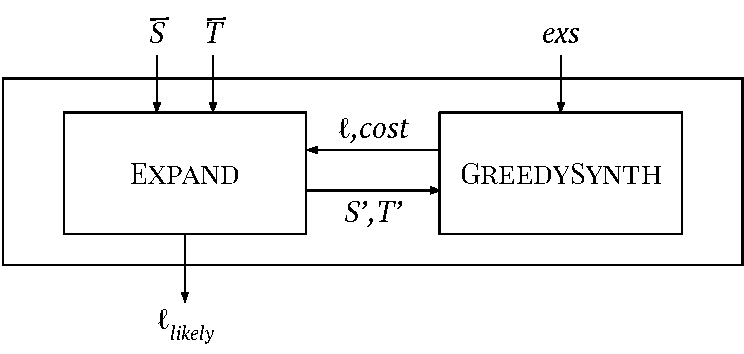
\includegraphics[width=.5\textwidth]{high-level-algorithm.pdf}
  \caption{Schematic Diagram for our symmetric lens synthesis algorithm. Regular
    expressions \Regex and \RegexAlt, and a set of examples \Examples, are
    provided as input. \RXSearch searches through stochastic regular expression
    pairs, equivalent to the originals, and proposes them to \GreedySynth.
    \GreedySynth finds a lens, typed between the generated equivalent pairs.
    When \RXSearch determines it has an optimal lens, it returns that lens.}
  \label{fig:high-level-algorithm}
\end{figure}

With simple symmetric lenses and SREs in hand, we develop a new algorithm for
synthesizing likely lenses, based on the previous algorithm for synthesizing
bijective lenses. This algorithm is constructed from \RXSearch and \GreedySynth,
a pair of collaborating search procedures, shown in
Figure~\ref{fig:high-level-algorithm}. Given source and target SREs $S$ and $T$,
the \RXSearch searches for two \emph{related} SREs $S'$ and $T'$ that are
\emph{compatible} (a heuristic that estimates the likelihood our second
algorithm will succeed). $S'$ and $T'$ are related in the sense that they define
the same regular sets as $S$ and $T$ (respectively) and the distribution of
strings is identical. Indeed, we guarantee these two properties by implementing
a search procedure that obeys the star semi-ring axioms of regular expression
equivalence, and which we show does not alter the probability distributions of
the languages.

Given the two compatible SREs, \GreedySynth uses a greedy, type-directed
algorithm find a likely lens between them. If algorithm estimates that the lens
it has discovered is more likely than any future lens it can possibly find, the
search terminates. Otherwise, this lens is stored away (if it is the best found
so far) and the search continues with \RXSearch again.

We implemented this\bcp{which?} algorithm and evaluated its effectiveness on a
range of benchmarks, including data cleaning tasks taken from Flash Fill,
information extraction tasks taken from Augeas, and ad-hoc format
synchronization tasks taken from a variety of locations\footnote{The majority of
  these format synchronization tasks were found from the following index:
  \url{http://fileformats.archiveteam.org/wiki/Electronic_File_Formats}}.

In summary, our main contributions are:
\begin{itemize}
\item We define the space of simple symmetric lenses, which lies between
  asymmetric lenses and full symmetric lenses and has the useful property that
  its members don't have any internal state (\S\ref{sec:overview}). 
\item We show how to synthesize simple symmetric lenses (including all asymmetric lenses as a special case),
using a novel application of stochastic regular expressions to guide the search process.  In particular, we
show that the RE star semi-ring equivalences remain valid when their semantics
are enriched by distributions (\S\ref{sec:synthesis}).
\item We extend the Boomerang implementation with simple symmetric lenses,
  showing that they can easily be combined with a rich variety of other lens
  extensions including quotients and matching lenses. We evaluate our
  implementation over a set of benchmarks drawn from data cleaning, information
  extraction, and file synchronization tasks and demonstrate that we can
  synthesize all of them in under half a minute (\S\ref{sec:evaluation}).
%
  We also analyze the gap between simple and full symmetric lenses
  empirically and argue that simple ones suffice for many applications.
\item We show that the class of simple lenses can be characterized
  semantically as the subset of full symmetric lenses for which a simple
  ``forgetfulness'' property holds (\S\ref{sec:related}).  \bcp{I suggest
    splitting this out into its own section, since there is other related
    work that we'll want to discuss in a Related Work section.}
\end{itemize}

%Such synthesis efforts
%make it easier to use lenses as programmers do not need to be familiar with the syntax
%of a new language, and even advanced users can benefit from the productivity boost.

\noindent

% state of the world
% end introduction

% begin overview
\section{Overview}
\label{sec:overview}

\begin{figure}
  % https://tex.stackexchange.com/questions/168741/showing-two-listings-in-a-table-side-by-side
  \setbox0=\hbox{%
    \begin{minipage}{3.5in}
\begin{lstlisting}[
stringstyle=\upshape\sffamily
]
Jane Doe: 38000
John Public: 37500
\end{lstlisting}
    \end{minipage}
  }
  \savestack{\listingA}{\box0}

  \setbox0=\hbox{%
    \begin{minipage}{3.5in}
\begin{lstlisting}[
stringstyle=\upshape\sffamily
]
Name,Company
Jane Doe,Healthcare Inc.
John Public,Insurance Co.
\end{lstlisting}
    \end{minipage}
  }
  \savestack{\listingB}{\box0}

  \setbox0=\hbox{%
    \begin{minipage}{3.5in}
\begin{lstlisting}
let salary = number | "N/A"
let emp_salary = name . " " . name . ": " salary
let emp_salaries = "" | emp_salary . ("\n" emp_salary)*
\end{lstlisting}
    \end{minipage}
  }
  \savestack{\listingC}{\box0}

  \setbox0=\hbox{%
    \begin{minipage}{3.5in}
\begin{lstlisting}
let company = (name . ("Co." | "Inc." | "Ltd.")) | "UNK" in
let emp_ins = name . " " . name "," company in
let header = "Name,Company" in
let emp_insurance = header . ("\n" . emp_ins)*
\end{lstlisting}
    \end{minipage}
  }
  \savestack{\listingD}{\box0}
  
  \centering
  \resizebox{\columnwidth}{!}{%
    \begin{tabular}{|>{\columncolor{lightyellow}}c|>{\columncolor{lightgreen}}c|}
      \hline
      \texttt{company.mgmt} data file & \texttt{company.hr} data file \\
      \hline
      \listingA & \listingB \\
      \hline
      \cellcolor{vlightyellow}\texttt{company.mgmt} regular expression & 
      \cellcolor{vlightgreen}\texttt{company.hr}  regular expression\\
      \hline
      \cellcolor{vlightyellow}\listingC & \cellcolor{vlightgreen}\listingD \\
      \hline
    \end{tabular}
  }
  \caption{Hypothetical example data files and corresponding regular expressions
  used by management and HR at a US company to represent employee salaries and health
  insurance providers, respectively. \ksf{Why
  is \lstinline{emp_salaries} written with an or instead of just using
  the star operator? Can we simplify?} }  
  \label{fig:minimized-representations}
\end{figure}

In this section, we give an overview of simple symmetric lenses and
our corresponding synthesis algorithm using an example drawn from a
hypothetical U.S. company.  In this company, management and
human resources (HR) store information about employees in separate files:
management records the names of employees and their salaries while
HR stores the names of employees and their health
insurance providers.  Figure~\ref{fig:minimized-representations} gives
examples of the two types of files and regular expressions describing
the two formats.
The company uses simple symmetric lenses to keep these files synchronized.
If management adds a new employee, ``Chris Roe: 32500'',  a lens adds 
the corresponding entry ``Chris Roe, UNK'' to HR's file.  The
sentinel value ``UNK'' represents the fact that the employee's
insurance company is currently unknown.  A similar update happens if
HR adds a new employee before management, in which case the sentinel
value ``N/A'' reflects the unknown salary information\bcp{can we just use
  ``UNKNOWN'' on both sides?  Or is there some reason to make it more
  complicated?} 
Furthermore, if HR
corrects an error in an employee's name, say changing ``John Public''
to ``Jon Public'', the lens mirrors that name change in management's
file. Not all the data is mirrored, however. The management file 
is not updated in response to insurance changes, and the HR file
is oblivious to salary changes.  Simple symmetric lenses are
appropriate for keeping these two files synchronized because the files have
a mix of shared and unshared information.

%Consider the previously
%described goal of keeping Linux cron jobs (crontab) and Windows Scheduled Tasks
%(scheduled.job) synchronized. These are each formats specifying when to run
%recurring tasks. For the sake of exposition, we use simplified versions crontab
%and scheduled.job formats, with examples and corresponding regular expressions
%shown in Figure~\ref{fig:minimized-representations}. Each file contains a list
%of tasks set to run at specific times every hour. In both formats, users
%can either provide specific minutes at which they want the program to run, or they
%can specify that the program should run at every minute.
%
%We wish for the jobs to be synchronized across our Windows and Linux devices.
%However, the commands that need to be run are typically different for each
%device. Paths are different in Windows and Linux, and, while there is typically a
%Windows equvialent for a Linux command, that equivalent command is not always
%named the same thing. So, while we want to be able to have the same number of
%commands, with the commands running at the same times, we don't want to
%align the actual commands that are run.

\subsection{Simple Symmetric Lenses}
A simple symmetric lens between formats described by types $\Regex$
and $\RegexAlt$ 
is defined by four functions\bcp{I think a picture would be helpful.  I can probably
  make one pretty easily by tweaking the one from the original symmetric paper.}

%\begin{enumerate}
%\item $\CreateR \OfType \Regex \rightarrow \RegexAlt$
%\item $\CreateL \OfType \RegexAlt \rightarrow \Regex$
%\item $\PutR \OfType \Regex \rightarrow \RegexAlt \rightarrow \RegexAlt$
%\item $\PutL \OfType \RegexAlt \rightarrow \Regex \rightarrow \Regex$
%\end{enumerate}

\begin{gather}
 \tag{1}
 \mbox{$\CreateR \OfType \Regex \rightarrow \RegexAlt$}\\
 \tag{2}
 \mbox{$\CreateL \OfType \RegexAlt \rightarrow \Regex$}\\
 \tag{3}
 \mbox{$\PutR \OfType \Regex \rightarrow \RegexAlt \rightarrow \RegexAlt$}\\
 \tag{4}
 \mbox{$\PutL \OfType \RegexAlt \rightarrow \Regex \rightarrow \Regex$}
\end{gather}

\noindent
that collectively satisfy four ``round-tripping'' laws: 
\begin{gather}
  \tag{\CreatePutRL}
  \PutLOf{(\CreateROf{s})}{s} = s\\
  \tag{\CreatePutLR}
  \PutROf{(\CreateLOf{t})}{t} = t\\
  \tag{\PutRL}
  \PutLOf{(\PutROf{s}{t})}{s} = s\\
  \tag{\PutLR}
  \PutROf{(\PutLOf{t}{s})}{t} = t
\end{gather}
\noindent
The two create functions provide default values for times when
data appears on one side but not the other (\EG, the ``N/A'' salary
entry added to the management file when HR inserts a new employee).
The two put functions propagate edits from one format to the
other by combining the change from one file with the previous value
from the other file. The roundtripping laws guarantee that identify edits to one file do
not change the data in the other file. 


%%For synchronization, when the original company.hr or company.mgmt
%%file is created, a synchronized file of the other form is created
%%from it with $\CreateR$ or $\CreateL$ (depending on which file was
%%initially created). On future edits, changes are made with the puts,
%%a \PutR would propagate the shared information from the company.hr
%%file, and knit it together with the information specific to the company.mgmt file.

We use regular expressions to denote the types of data formats, and we
impose a typing discipline on our lenses.  Specifically, if 
$\Regex$ and $\RegexAlt$ are regular expressions, then the notation
\lstinline{$\Lens$ : $\Regex \Leftrightarrow \RegexAlt$} indicates that $\Lens$
is a simple symmetric lens between $\LanguageOf{\Regex}$ and
$\LanguageOf{\RegexAlt}$. 
When clear from context, we use the term \textit{lens} to denote a
simple symmetric lens.


\subsection{Simple Symmetric Lens Combinators} 
Generally, we do not expect programmers to define simple symmetric lenses by
writing the four functions by hand and showing they satisfy the
roundtripping laws.  Instead, we provide simple symmetric lens
combinators to build up the requisite lenses from simpler ones.
We briefly explain a selection of these combinators by using them to
define a lens between 
the two employee data formats in Figure~\ref{fig:minimized-representations}. 
The finished lens, which appears in Figure~\ref{fig:example_lens}, has
the type 
\lstinline{emp_salaries} $\Leftrightarrow$ \lstinline{emp_insurance}, where
\lstinline{emp_salaries} and \lstinline{emp_insurance} are regular
expressions defined in Figure~\ref{fig:minimized-representations}. 


The simplest combinator is the identity lens \IdentityLens, which takes as an
argument a regular expression $\Regex$ and performs an identity mapping on data
matching $\Regex$. The identity lens fully connects the
corresponding data in the two formats: when one format is
updated, the other format gets the exact same value. In our example,
when a \lstinline{name} is updated in one file, the identify lens ensures it is
also updated in the other file. 

%
\begin{lstlisting}
id(name) : name $\Leftrightarrow$ name
\end{lstlisting}
%

In contrast to the identity lens, the disconnect lens, \Disconnect, leaves data
unconnected.\bcp{Can we call it ``disconnect''?} The disconnect lens takes four arguments: two regular 
expressions and two strings. The regular expressions specify the
formats of the corresponding data on the two sides while the strings provide default
values.  In our extended example, 
the \lstinline{salary} and \lstinline{company} fields are independent,
so we use the disconnect lens to relate them.
The defaults are strings that indicate the information is missing.
%
\begin{lstlisting}
disc(salary, company, "N/A", "UNK") : salary $\Leftrightarrow$ company
\end{lstlisting}
%
The insert \lstinline{ins} and delete \lstinline{del} lenses are
syntactic sugar for uses of the disconnect lens in which a string
constant is omitted entirely from the source and target formats,
respectively. \ksf{Are these in the right order?}
\begin{lstlisting}
 ins($t$) = disc("", $t$, "", $t$)
 del($s$) = disc($s$, "", $s$, "")
\end{lstlisting}

Finally, there are a number of standard lenses that compositionally
construct more complex lenses from simpler ones.  These combinators include 
\lstinline{concat} for concatenation, 
\lstinline{or} for variation, and
\IterateLens for sequences.
We usually write \lstinline{concat} using an infix
notation \lstinline{$\Lens_1$ . $\Lens_2$}
as in:
%
\begin{lstlisting}
id(name) . ins(",") . id(name) . del(": ") . ins(",")
\end{lstlisting}
% concat(ins(header),employees_lens) : emp_salaries $\Leftrightarrow$ emp_insurance
%
which appears in the definition of the \lstinline{name_lens} in our
running example. 
%\ksf{I don't think this example is necessary.}
%Data can also appear in multiple forms. For example,
%a list of employees with insurance information can either be empty or
%be a sequence of employee/insurance records: \ksf{This example is
%vacuous as you could eliminate the or in favor of the *.  Do somethign
%else to introduce or?}
%
%\begin{lstlisting}
%or(id(""),employees_lens) : emp_salaries $\Leftrightarrow$ "" | ("\n" emp_ins) . ("\n" emp_ins)*
%\end{lstlisting}
The \IterateLens lens also appears in our running example, where it
synchronizes data for a list of employees when given a
lens \lstinline{employee_lens} that synchronizes  data for a single employee:
%
\begin{lstlisting}
iterate(id("\n") . employee_lens) : ("\n" . emp_salary)$^*$ $\Leftrightarrow$ ("\n" . emp_ins)$^*$
\end{lstlisting}
%

\begin{figure}
\begin{lstlisting}
let name_lens = id(name) . ins(",") . id(name) . del(": ") . ins(",") in
let employee_lens = name_lens . disc(salary,company,"N/A","UNK") in
let employees_lens = ins("\n") . employee_lens . iterate(id("\n") . employee_lens) in
ins(header) . employees_lens : emp_salaries $\Leftrightarrow$ emp_insurance
\end{lstlisting}
%\ksf{I don't think this is necesssary.}
%let emp_lens = or(id(""),employees_lens) in
  \caption{A lens, written in our language for building simple symmetric lenses
    on string data, that synchronizes management and HR employee files.
    Note that we can annotate our lenses with types, to confirm the lens
    operates on the languages of the regular expressions. In this work, we
    synthesize the lens itself from such regular expressions.}
  \label{fig:example_lens}
\end{figure}

% Using these combinators, we can build up a lens that synchronizes
% management and HR employee files. 


We provide typing rules for each of the simple symmetric combinators,
most of which are syntax directed.  There is one additional
typing rule, which allows us to use equivalence relations on regular
expressions to convert the type of any lens to a semantically equal
but syntactically different pair of regular expressions.  The flexibility this
type equivalence rule provides is useful when a different
representation of a regular expression would facilitate synthesis. 

%%\ksf{Do we need to use
%%type equivalence to type the employee example?  If so, perhaps we
%%should explain her}
%%
%%This lens uses one typing rule not previously
%%mentioned: type equivalence. While \lstinline{scheduled_job} is a equivalent to
%%a regular expression with an outermost disjunction, it is not syntactically
%%equivalent to one. Without type equivalence, the provided lens wouldn't actually
%%be well-typed, but type equivalence states that if a lens is typed between a
%%pair of regular expressions, it is also typed between an equivalent pair.

Note that, while the synchronization task for our running example is quite simple, the
requisite lens is relatively complex. Furthermore, this complexity is
inherent in manually writing simple symmetric lenses because the
lenses must precisely describe the portions of the data that should be
connected and those that should be disconnected.  For disconnected
pieces, the lens must further specifiy appropriate defaults.



\subsection{Synthesizing Symmetric Lenses}

To alleviate the difficulty of manually writing simple symmetric
lenses, we wish to synthesize them instead. Given 
a pair of regular expressions and a set of input-output examples, we want to
find a simple symmetric lens that is typed by the regular expression
pair and satisfies the input/output examples. We call such a lens
a \emph{satisfying lens}.
In our running example, we wish to
synthesize a lens between \lstinline{emp_salaries} and \lstinline{emp_insurance},
using as an input-output example the data in
Figure~\ref{fig:minimized-representations}.  The algorithm uses such
examples to find suitable defaults for \Disconnect lenses and to
figure out how to match data that could be synchronised in multiple
ways. 

A challenge is that the simple symmetric lens combinators permit many
well-typed lenses
between a given pair of regular expressions. For example, 
Figure~\ref{fig:example_lens} gives one possible lens between regular
expressions  \lstinline{emp_salaries} and \lstinline{emp_insurance},
but 
%
\begin{lstlisting}
disc(emp_salaries,emp_insurance,rep(emp_salaries),rep(emp_insurance))
\end{lstlisting}
%
is another valid lens (where \lstinline{rep($\Regex$)} is a string in the
language of $\Regex$). Furthermore, adding the input-output example in
Figure~\ref{fig:minimized-representations} 
helps, but only a little, because it requires many examples to rule
out all the possible occurrences of nested \Disconnect lenses,
particularly in complex formats. 
%\ksf{I don't understand the following.  We shouldn't explain the issue in
%terms of \PutR and \PutL as we are focused on the combinators rather
%than the raw functions.}
%The default strings given to \Disconnect merely need to be the strings
%in the input-output examples, and the lens will still satisfy the
%specification.  While the disconnect lens is prohibited by two
%examples, or by a carefully chosen input-output example on \PutR
%or \PutL, this problem continues presenting itself for the sublenses,
%and is highlighted even more on larger formats.
While
we could ask programmers to provide detailed and precise specifications for their
synthesis tasks, we would prefer the algorithm to choose the right lens
automatically. Instead of merely finding \emph{any} satisfying lens, we wish to
synthesize a satisfying lens that is likely to please the user.  

But what is a likely satisfying lens? We propose that a satisfying
lens is more likely if it connects more data between the two
formats, \IE, by using an identity rather than a disconnect lens.  The
likeliest satisfying lenses would connect as much data as
possible. More formally, we propose that the likelihood of a
satisfying lens is the expected number of bits required to recover
data in one format from synchronized data in the other.  Higher
likelihoods correspond to fewer numbers of bits. In more
detail, we say that two strings $s$ and $t$ are \emph{synchronized
according to lens $l$} if $l.\PutR\ s\ t = t$ and $l.\PutL\ t\ s = s$.\footnote{
The notation $l.\PutR$ extracts the \PutR function from simple
symmetric lens $l$; similarly for \PutL.}  We say that we
can \emph{recover} $s$ from $t$ using bits $b$ and lens $l$ if we can
reconstruct $s$ from $t$, $b$, and $l$.  For example, given
the \IdentityLens{} lens, we can recover $s$ from $t$ using no bits
because in this case, $s$ is just $t$.  In contrast, given
the \Disconnect{} lens, we need enough bits to fully encode $s$ in
order to recover it from $t$ because $t$ contains no useful
information.  This calculation shows that if both \IdentityLens{}
and \Disconnect{} are satisfying lenses, then \IdentityLens{} is more
likely.

The expected number of bits required to recover data is a
well-known concept in information theory: it is the \emph{entropy} of
the data. Calculating the 
entropy of data requires a probability distribution over the
space of possible values for the data.  Specifically,
given a set $S$ and a probability distribution over that set $P
\OfType S \rightarrow \Reals$, the entropy of the $(S,P)$ pair is $-\Sigma_{s\in
  S}P(s)\Log_2P(s)$. 

In our setting, we already have a way of expressing sets of data:
regular expressions.  What we need is a way to express probability
distributions over that data.
To that end, we adopt \emph{stochastic regular expressions}\ksf{is
there a citation?}, 
which are regular expressions where each operator is annotated with a
probability.  Stochastic regular expressions
allow us to jointly specify the allowable data and give a probability
distribution over it.  From this information, we can calculate the
entropy of the stochastic regular expression. 

This infrastructure gives us what we need to find likely
satisfying lenses from a collection of satisfying lenses.  All such
lenses must synchronize data between the same two 
stochastic regular expressions $\Regex$ and $\RegexAlt$.
For any such lens $\Lens$, we can calculate the expected number of
bits required 
to recover a string $s$ in $\LanguageOf{\Regex}$ from a synchronized
string $t$ in $\LanguageOf{\RegexAlt}$. 
This expected number of bits is just the conditional entropy of
$\Regex$ given $\RegexAlt$ and $\Lens$. 
To ensure symmetry, the likelihood we assign to $\Lens$ is the sum of 
the conditional entropy of $\Regex$ given $\RegexAlt$ and $\Lens$ and
the conditional entropy of $\RegexAlt$ given $\Regex$ and $\Lens$.

To obtain stochastic regular expressions from the plain regular
expressions that we expect users to supply, we use a heurstic 
that attempts to assign
probability annotations that give each string in the language equal
probablity.  We can also take as input a stochastic regular
expression rather than a plain one, which allows the user to
specify a data-specific probability distribution.  Alternatively,
the user could provide a large suite of example data from which we
could infer the necessary annotations to model the supplied data. 

Now that we have a way to calculate likelihood, we need a way to search for
it.
Previous work on synthesis~\ksf{add citations} has shown
that we can use types to dramatically restrict the search space and
improve the effectiveness of synthesis.  In our setting, types are
pairs of stochastic regular expressions, which come with a rich
algebraic structure that makes each regular expression semantically
equal to infinitely many others.  To tame that search space and
leverage the benefits of type-directed synthesis, we split our
algorithm into two communicating synthesizers following earlier
work~\cite{quotient-lens-synthesis}.  The first
synthesizer, \RXSearch, navigates the space of semantically equivalent
regular expressions by iteratively applying rewrite rules that
preserve both the semantics and the probability
distributions of those stochastic regular expressions. \RXSearch
ranks pairs of stochastic regular expressions 
by the number of rewrite rule applications required to obtain the pair
from the stochastic regular expressions given as input. It passes the
pairs off to the second synthesizer, \GreedySynth, in rank order with
the smallest first.

At a high level, \GreedySynth looks for lenses between a given pair of
stochastic regular expressions $\Regex$ and $\RegexAlt$ that have the
highest likelihood by performing a type-directed search. 
In more detail, \GreedySynth first uses type equalities based on semiring 
equivalences (ignoring the star semiring equivalences that are managed
by \RXSearch) to normalize the
stochastic regular expressions provided by \RXSearch into 
\emph{stochastic n-ary DNF regular expressions}.  
Then, \GreedySynth uses the syntax of these n-ary DNF regular
expressions to find highly normalized lenses, in a
form we call \emph{simple symmetric n-ary DNF lenses}.  These lenses include
neither a composition operator nor a type equivalence rule.  These
restrictions mean that each simple symmetric n-ary DNF lens is typed
by a single pair of stochastic n-ary DNF regular expressions and 
\GreedySynth's search space for a given pair of regular expressions is
finite.  The variations that \GreedySynth 
considers include choosing between \IdentityLens{} and  \Disconnect
lenses and deciding how to match multiple occurrences of the same kind
of data, \EG, the two occurrences of \lstinline{name} in the
management and HR data formats (we want to map first names to first
names and last names to last names). 
Finally, \GreedySynth converts this lens 
back into a simple symmetric lens by converting the n-ary forms into
the binary forms provided in the surface language.  

As an example of the partnership between \RXSearch and \GreedySynth,
consider the lens shown in Figure~\ref{fig:example_lens}. 
Inferring this lens requires \RXSearch to use a star semiring axiom to
rewrite the regular expression \lstinline{("\n" . emp_salary)$^*$} within
\lstinline{emp_salaries} into 
\lstinline{"" | (("\n" . emp_salary). ("\n" . emp_salary)$^*$)} 
so that \GreedySynth can find the appropriate lens.  

Our strategy of communicating synthesizers gives us a way to
enumerate pairs of stochastic regular expressions of increasing
rank and to efficiently search through them, but it poses a
problem: when do we stop? We may have found a promising lens
between a pair of stochastic regular expressions, but a different 
pair we haven't yet discovered may give rise to an even better lens. 
Or, we may have found a promising lens between a given pair of
stochastic regular expressions, but the discovered lens is not 
acceptable to the users. 

Our algorithm must resolve a three-way tension between the quality of
the inferred lens, the number of examples the user must provide to
eliminate unwanted lenses, and the amount of time it takes to return a
result.  For example, if the algorithm has already found the lens in
Figure~\ref{fig:example_lens}, we don't want to spend a lot of time
searching for an even better lens.

To resolve this tension, \RXSearch uses heuristics to judge whether to
return the current best satisfying lens to the user or to pass the
next set of unrollings to \GreedySynth.
The heuristics favor stopping if the current best satisfying
lens has relatively high likelihood, indicating the lens is very promising.
The heuristics also favor stopping if \RXSearch 
has delievered to \GreedySynth all pairs of stochastic regular
expressions at a given rank and there is a large number of pairs at the next
rank because searching through all such pairs will take a long time.
With this approach, the algorithm can quickly respond with a satisfying
lens with relatively high likelihood.  If users are unhappy with the result, they can refine the
search by supplying additional examples, which serve both to rule out
the previously proposed lens(es) and to reduce the size of the search
space by cutting down on the number of satisfying lenses.


%Consider the trivial lens
%\lstinline{disc(emp_salary,emp_row,rep(emp_salary),rep(emp_row))}. As this is
%the disconnect lens, the cost of each side is the entropy of the data format, so
%the total cost is $\EntropyOf{\lstinline{emp_salary}} +
%\EntropyOf{\lstinline{emp_row}}}$. \lstinline{emp_salary} contains strictly more
%imformation than \EntropyOf{\lstinline{": " . salary}}, and \lstinline{emp_row}
%contains strictly more information than \EntropyOf{\lstinline{": " . salary}},
%so by our metric \lstinline{single_emp_map} is preferable to the disconnect
%lens.

%Not sure we need this level of detail after all.
%\afm{calculations for cost of various lenses between \lstinline{emp_salary} and
%  \lstinline{emp_row}} Consider the lens \lstinline{single_emp_map} between
%\lstinline{emp_salary} and \lstinline{emp_row}. Given this lens, the expected
%entropy of recovering the left format from the right
%($\EntropyOf{\lstinline{emp_salary} \Given \lstinline{emp_row},
%  \lstinline{single_emp_map} }$) is the sum of the expected entropy of
%recovering each of its subcomponents, $\EntropyOf{\lstinline{emp_salary} \Given
%  \lstinline{emp_row}, \lstinline{single_emp_map} } = \EntropyOf{\lstinline{name
%    . " " . name} \Given \lstinline{name . "," . name}, \lstinline{name_map}
%}$\\ + $\EntropyOf{\lstinline{": " . salary} \Given
%  \lstinline{"," . company}, \lstinline{disc(salary,company,"UNSET","UNSET")}
%}$.
%
%The entropy of the identity lens is zero. As the two formats are in bijective
%correspondence, we know exactly which string is present in the left-hand format.
%The entropy of the disconnect lens is just the entropy of
%\lstinline{": " . salary}.  Knowing which string is present in the right-hand
%format tells us nothing about what string is present in the left-hand format. So
%$\EntropyOf{\lstinline{emp_salary} \Given \lstinline{emp_row},
%  \lstinline{single_emp_map} } = \EntropyOf{\lstinline{": " . salary} }$
%
%Analogously, $\EntropyOf{\lstinline{emp_row} \Given \lstinline{emp_salary},
%  \lstinline{single_emp_map} }$ is just $\EntropyOf{\lstinline{"," . company}
%}$, so the total cost of the lens is $\EntropyOf{\lstinline{": " . salary}} +
%\EntropyOf{\lstinline{"," . company}}$

%Consider the trivial lens
%\lstinline{disc(emp_salary,emp_row,rep(emp_salary),rep(emp_row))}. As this is
%the disconnect lens, the cost of each side is the entropy of the data format, so
%the total cost is $\EntropyOf{\lstinline{emp_salary}} +
%\EntropyOf{\lstinline{emp_row}}$. \lstinline{emp_salary} contains strictly more
%imformation than \EntropyOf{\lstinline{": " . salary}}, and \lstinline{emp_row}
%contains strictly more information than \EntropyOf{\lstinline{": " . salary}},
%so by our metric \lstinline{single_emp_map} is preferable to the disconnect
%lens.
Consider the trivial lens
\lstinline{disc(emp_salary,emp_row,rep(emp_salary),rep(emp_row))}. As this is
the disconnect lens, the cost of each side is the entropy of the data format, so
the total cost is $\EntropyOf{\lstinline{emp_salary} } +
\EntropyOf{\lstinline{emp_row}}$. \lstinline{emp_salary} contains strictly more
imformation than $\EntropyOf{\lstinline{": " . salary}}$, and
\lstinline{emp_row} contains strictly more information than
\EntropyOf{\lstinline{": " . salary}}, so by our metric
\lstinline{single_emp_map} is preferable to the disconnect lens.
% end overview

% begin stoch-rx
% end stoch-rx

\section{Stochastic Regular Expressions}
\label{sec:srx}
Important to our algorithm is finding the expected number of bits needed to
recover a string in one data source from a synchronized string in the other data
source. To do this, we must first develop a probability model for our language.
We do this with \emph{stochastic regular expressions}, regular expressions
annotated with probability information. With this, we can jointly express a
language and a probability distribution over that language.

\begin{center}
  \begin{tabular}{rcl}
    \Regex{},\RegexAlt{}
    & \GEq{} & $\String$ \\
    & \GBar{} & $\emptyset$ \\
    & \GBar{} & $\PRegexStar{\Regex}{p}$ \\
    & \GBar{} & $\RegexConcat{\Regex_1}{\Regex_2}$ \\
    & \GBar{} & $\PRegexOr{\Regex_1}{\Regex_2}{p}$
  \end{tabular}
\end{center}

The language is defined like the regular expression without probability
annotations would be.  The probabilities are defined as follows:
\begin{center}
  \begin{tabular}{rcl}
    $\ProbabilityOf{\String}{\String''}$
    & =
    & $\begin{cases*}1 & if $\String = \String''$\\ 0 & otherwise\end{cases*}$ \\
    
    $\ProbabilityOf{\emptyset}{\String}$
    & =
    & $0$ \\
    
    $\ProbabilityOf{\RegexConcat{\Regex_1}{\Regex_2}}{s}$

    & =
    & $\Sigma_{\String = \String_1\String_2}\ProbabilityOf{\Regex_1}{\String_1}*\ProbabilityOf{\Regex_2}{\String_2}$ \\
    
    $\ProbabilityOf{\PRegexOr{\Regex_1}{\Regex_2}{\Probability}}{\String}$
    & =
    & $\Probability * \ProbabilityOf{\Regex_1}{\String} +
      (1-\Probability) * \ProbabilityOf{\Regex_2}{\String}$\\
    
    $\ProbabilityOf{\PRegexStar{\Regex}{\Probability}}{\String}$
    & =
    & $\Sigma_n \Sigma_{\String = \String_1 \ldots \String_n}\Probability^n*(1-\Probability)*\Pi_{i=1}^n\ProbabilityOf{\Regex}{\String_i}$\\
  \end{tabular}
\end{center}
In the stochastic regular expression
$\PRegexOr{\Regex_1}{\Regex_2}{\Probability}$, the annotation \Probability
represents the likelihood the string is in $\Regex_1$. In the stochastic regular
expression $\PRegexStar{\Regex}{\Probability}$, the annotation \Probability
how much more likely having a string involving more than $n$ iterations is than
having a string involving $n$ iterations.

\subsection{Stochastic Regular Expression Equivalences}
$\RXSearch$ needs to be able to find equivalent stochastic regular expressions.
However, as of yet, there is no syntactic means to reason about stochastic
regular expression equivalence. We extend the \emph{star-semiring} equivalences
to stochastic regular expressions.

\begin{center}
  \begin{tabular}{@{}r@{\hspace{1em}}c@{\hspace{1em}}l@{}r@{}}
    \PRegexOr{\Regex}{\emptyset}{1} & $\SSREquiv$ & \Regex{} & \OrIdentityRule{} \\
    $\RegexConcat{\Regex}{\emptyset}$ & $\SSREquiv$ & $\emptyset$ & \EmptyProjectionRightRule{} \\
    $\RegexConcat{\emptyset}{\Regex}$ & $\SSREquiv$ & $\emptyset$ & \EmptyProjectionLeftRule{} \\
    \RegexConcat{(\RegexConcat{\Regex{}}{\Regex'})}{\Regex''} & $\SSREquiv$ & \RegexConcat{\Regex{}}{(\RegexConcat{\Regex'}{\Regex''})} & \ConcatAssocRule{}  \\
    \PRegexOr{(\PRegexOr{\Regex}{\Regex'}{\Probability_1})}{\Regex''}{\Probability_2} & $\SSREquiv$ & \PRegexOr{\Regex}{(\PRegexOr{\Regex'}{\Regex''}{\frac{(1-\Probability_1)*\Probability_2}{1 - \Probability_1 * \Probability_2}})}{\Probability_1*\Probability_2} & \OrAssociativityRule{}  \\
    \PRegexOr{\Regex{}}{\RegexAlt{}}{\Probability} & $\SSREquiv$ & \PRegexOr{\RegexAlt{}}{\Regex{}}{1-\Probability} & \OrCommutativityRule{}\\
    \RegexConcat{\Regex{}}{(\PRegexOr{\Regex{}'}{\Regex{}''}{\Probability})} & $\SSREquiv$ & \PRegexOr{(\RegexConcat{\Regex{}}{\Regex{}'})}{(\RegexConcat{\Regex{}}{\Regex{}''})}{\Probability} & \DistributivityLeftRule{} \\
    \RegexConcat{(\PRegexOr{\Regex{}'}{\Regex{}''}{\Probability})}{\Regex{}} & $\SSREquiv$ & \PRegexOr{(\RegexConcat{\Regex{}'}{\Regex{}})}{(\RegexConcat{\Regex{}''}{\Regex{}})}{\Probability} & \DistributivityRightRule{} \\
    \RegexConcat{\EmptyString{}}{\Regex{}} & $\SSREquiv$ & \Regex{} & \ConcatIdentityLeftRule{} \\
    \RegexConcat{\Regex{}}{\EmptyString{}} & $\SSREquiv$ & \Regex{} & \ConcatIdentityRightRule{} \\
    \PRegexStar{\Regex{}}{\Probability} & $\SSREquiv$ & \PRegexOr{\EmptyString{}}{(\RegexConcat{\Regex{}}{\PRegexStar{\Regex{}}{\Probability}})}{1-\Probability} & \UnrollstarLeftRule{} \\
    \PRegexStar{\Regex{}}{\Probability} & $\SSREquiv$ & \PRegexOr{\EmptyString{}}{(\RegexConcat{\PRegexStar{{\Regex{}}}{\Probability}}{\Regex{}})}{1-\Probability} & \UnrollstarRightRule{} 
  \end{tabular}
\end{center}

\begin{theorem}
  If $\Regex \SSREquiv \RegexAlt$ then $\ProbabilityOf{\Regex}{\String} =
  \ProbabilityOf{\RegexAlt}{\String}$, for all strings $\String \in \LanguageOf{\Regex}$.
\end{theorem}

\subsection{Stochastic Regular Expression Entropy}
The entropy of a stochastic regular expression can be computed directly from its
syntax, when the stochastic regular expression is unambiguous and contains only
nonempty subcomponents.
\begin{center}
  \begin{tabular}{rcl}
    $\EntropyOf{s}$
    & =
    & 1\\
    
    $\EntropyOf{\PRegexStar{\Regex}{\Probability}}$
    & =
    & $\frac{\Probability}{1-\Probability}(\EntropyOf{\Regex} - \Log_2\Probability)
      - \Log_2(1-\Probability)$\\
    
    $\EntropyOf{\PRegexConcat{\Regex}{\RegexAlt}}$
    & =
    & \EntropyOf{\Regex} + \EntropyOf{\RegexAlt}\\
    
    $\EntropyOf{\PRegexOr{\Regex}{\RegexAlt}{\Probability}}$
    & =
    & $\Probability*(\EntropyOf{\Regex} - \Log_2(\Probability)) + (1-\Probability)*(\EntropyOf{\RegexAlt} - \Log_2(1-\Probability))$\\
  \end{tabular}
\end{center}
We have proven\bcp{This is a POPL paper: Proofs of important theorems should
be included.} that this syntactic computation corresponds to the entropy of the
stochastic regular expression.

\begin{theorem}
  \label{thm:correct_entropy}
  If $\Regex$ is unambiguous and contains no empty subcomponents,
  $\EntropyOf{\Regex}$ is the entropy of $\Regex$.
\end{theorem}

% \caption{Regular Expression Equivalences}
% \label{fig:regex-equivalence-rules}

% begin ssl
\section{Simple Symmetric String Lenses}
\label{sec:ssl}
We now give a formal description of all the combinators in our symmetric lens
language. These lens terms are typed between pairs of stochastic regular
expressions: the typing judgment $\Lens \OfType \Regex \Leftrightarrow
\RegexAlt$ means that $\Lens$ is a well typed lens between $\LanguageOf{\Regex}$
and $\LanguageOf{\RegexAlt}$. These lens terms can also be typed between regular
expressions, but we present in terms of stochastic regular expressions to assist
in describing the entropy of the lenses.

\begin{center}
  \begin{tabular}{l@{\ }l@{\ }l@{\ }l}
    % REGEX
    \Lens{} & \GEq{} & & $\IdentityLensOf{\Regex}$\\
            & & \GBar{} & $\DisconnectOf{\Regex}{\RegexAlt}{\String}{\StringAlt}$ \\
            & & \GBar{} & $\IterateLensOf{\Lens}$ \\
            & & \GBar{} & $\ConcatLensOf{\Lens_1}{\Lens_2}$ \\
            & & \GBar{} & $\SwapLensOf{\Lens_1}{\Lens_2}$ \\
            & & \GBar{} & $\OrLensOf{\Lens_1}{\Lens_2}$ \\
            & & \GBar{} & $\ComposeLensOf{\Lens_1}{\Lens_2}$ \\
            & & \GBar{} & $\MergeROf{\Lens_1}{\Lens_2}$ \\
            & & \GBar{} & $\MergeLOf{\Lens_1}{\Lens_2}$ \\
            & & \GBar{} & $\InvertOf{\Lens}$ \\
  \end{tabular}
\end{center}

We have already described over a number of these lenses in \S\ref{sec:overview}.
The compose lens $\Lens_1 ; \Lens_2$ composes two lenses sequentially, it
transforms from one data format to the other by first transforming to an
intermediate format, shared as the target of $\Lens_1$ and the source of
$\Lens_2$. The \MergeR lens combines two sublenses which share the same target.
Which lens gets used depends on what data is in the left-hand format, if it is
in the domain of $\Lens_1$ then $\Lens_1$ gets used, and similarly for
$\Lens_2$.  The \MergeL lens is symmetric to \MergeR, the two sublenses must
share the same source. Finally, $\InvertOf{\Lens}$ inverts a lens, \CreateR
becomes \CreateL and \PutR becomes \PutL, and vice-versa.

We now provide the typing derivations and semantics for these lenses. For
simplicity, we define the typing derivations and semantics only over unambiguous
regular expressions, even though some lenses can be defined over ambiguous
regular expressions (for example, the identity lens doesn't need any ambiguity
constraints).

\[
  \centering
  \inferrule*
  {
  }
  {
    \IdentityLensOf{\Regex} \OfType \Regex \Leftrightarrow \Regex
  }
\]
\begin{center}
  \begin{tabular}{@{}r@{\ }c@{\ }l@{}}
    $\CreateR{} \App s$ & = & $s$\\
    $\CreateL{} \App s$ & = & $s$\\
    $\PutR{} \App s_1 \App s_2$ & = & $s_1$\\
    $\PutL{} \App s_1 \App s_2$ & = & $s_1$
  \end{tabular}
\end{center}

Note that the identity lens ignores the second argument in the put functions.
Because the two formats are fully synchronized, no knowledge of the prior data
is needed.

\[
  \centering
  \inferrule*
  {
    \String \in \LanguageOf{\Regex}\\
    \StringAlt \in \LanguageOf{\RegexAlt}
  }
  {
    \DisconnectOf{\Regex}{\RegexAlt}{\String}{\StringAlt}
    \OfType \Regex \Leftrightarrow \RegexAlt
  }
\]
\begin{center}
  \begin{tabular}{@{}r@{\ }c@{\ }l@{}}
    $\CreateR{} \App \String'$ & = & $\StringAlt$\\
    $\CreateL{} \App \StringAlt'''''$ & = & $\String$\\
    $\PutR{} \App \String''' \App \StringAlt'$ & = & $\StringAlt'$\\
    $\PutL{} \App \StringAlt' \App \String'$ & = & $\String'$
  \end{tabular}
\end{center}
Just as the identity lens ignores the second argument in puts, disconnect lenses
ignore the first in both puts and creates.  The data is unsynchronized in these
two formats, information from one format doesn't impact the other.

\[
  \centering
  \inferrule*
  {
    \Lens_1 \OfType \Regex_1 \Leftrightarrow \RegexAlt_1\\
    \Lens_2 \OfType \Regex_2 \Leftrightarrow \RegexAlt_2
  }
  {
    \ConcatLensOf{\Lens_1}{\Lens_2} \OfType \Regex_1 \Concat \Regex_2
    \Leftrightarrow
    \RegexAlt_1 \Concat \RegexAlt_2
  }
\]
%\begin{center}
%  \begin{tabular}{@{}r@{\ }c@{\ }l@{}}
%    $\CreateR{} \App \String_1 \String_2$ & = & $(\Lens_1.\CreateROf{\String_1})(\Lens_2.\CreateROf{\String_2})$\\
%    $\CreateL{} \App \StringAlt_1 \StringAlt_2$ & = & $(\Lens_1.\CreateLOf{\StringAlt_1})(\Lens_2.\CreateLOf{\StringAlt_2})$\\
%    $\PutR{} \App (\String_1\String_2) \App (\StringAlt_1\StringAlt_2)$ & = & $(\Lens_1.\PutROf{\String_1}{\StringAlt_1})(\Lens_2.\PutROf{\String_2}{\StringAlt_2})$\\
%    $\PutL{} \App (\StringAlt_1\StringAlt_2) \App (\String_1\String_2)$ & = & $(\Lens_1.\PutLOf{\StringAlt_1}{\String_1})(\Lens_2.\PutLOf{\StringAlt_2}{\String_2})$\\
%  \end{tabular}
%\end{center}

Concat is similar to concatenation in existing string lens languages like
Boomerang.  For such terms, we do not provide the semantics, and merely refer
readers to existing work.

\[
  \centering
  \inferrule*
  {
    \Lens_1 \OfType \Regex_1 \Leftrightarrow \RegexAlt_1\\
    \Lens_2 \OfType \Regex_2 \Leftrightarrow \RegexAlt_2
  }
  {
    \SwapLensOf{\Lens_1}{\Lens_2} \OfType \Regex_1 \Concat \Regex_2
    \Leftrightarrow
    \RegexAlt_2 \Concat \RegexAlt_1
  }
\]
%\begin{center}
%  \begin{tabular}{@{}r@{\ }c@{\ }l@{}}
%    $\CreateR{} \App \String_1\String_2$ & = & $(\Lens_2.\CreateROf{\String_2})(\Lens_1.\CreateROf{\String_1})$\\
%    $\CreateL{} \App \StringAlt_2\StringAlt_1$ & = & $(\Lens_1.\CreateLOf{\StringAlt_1})(\Lens_2.\CreateLOf{\StringAlt_2})$\\
%    $\PutR{} \App (\String_1\String_2) \App (\StringAlt_2\StringAlt_1)$ & = & $(\Lens_2.\PutROf{\String_2}{\StringAlt_2})(\Lens_1.\PutROf{\String_1}{\StringAlt_1})$\\
%    $\PutL{} \App (\StringAlt_2\StringAlt_1) \App (\String_1\String_2)$ & = & $(\Lens_1.\PutLOf{\StringAlt_1}{\String_1})(\Lens_2.\PutLOf{\StringAlt_2}{\String_2})$\\
%  \end{tabular}
%\end{center}
The swap combinator is similar to concat, though the second regular expression
is swapped.

\[
  \centering
  \inferrule*
  {
    \Lens_1 \OfType \Regex_1 \Leftrightarrow \RegexAlt_1\\
    \Lens_2 \OfType \Regex_2 \Leftrightarrow \RegexAlt_2
  }
  {
    \OrLensOf{\Lens_1}{\Lens_2} \OfType
    \RegexOr{\Regex_1}{\Regex_2}
    \Leftrightarrow
    \RegexOr{\RegexAlt_1}{\RegexAlt_2}
  }
\]
\begin{center}
  \begin{tabular}{@{}r@{\ }c@{\ }l@{}}
    $\CreateR{} \App \String$
    & =
    & $\begin{cases*}
      \Lens_1.\CreateROf{\String} & if $\String\in\LanguageOf{\Regex_1}$\\
      \Lens_2.\CreateROf{\String} & if $\String\in\LanguageOf{\Regex_2}$
      \end{cases*}$\\
    
    $\CreateL{} \App \StringAlt$
    & =
    & $\begin{cases*}
      \Lens_1.\CreateLOf{\StringAlt} & if $\StringAlt\in\LanguageOf{\RegexAlt_1}$\\
      \Lens_2.\CreateLOf{\StringAlt} & if $\StringAlt\in\LanguageOf{\RegexAlt_2}$
      \end{cases*}$\\
    
    $\PutR{} \App \String \App \StringAlt$
    & =
    & $\begin{cases*}
        \Lens_1.\PutROf{\String}{\StringAlt} & if $\String\in\LanguageOf{\Regex_1} \BooleanAnd \StringAlt\in\LanguageOf{\RegexAlt_1}$\\
        \Lens_2.\PutROf{\String}{\StringAlt} & if $\String\in\LanguageOf{\Regex_2} \BooleanAnd \StringAlt\in\LanguageOf{\RegexAlt_2}$\\
        \Lens_1.\CreateROf{\String} & if $\String\in\LanguageOf{\Regex_1} \BooleanAnd \StringAlt\in\LanguageOf{\RegexAlt_2}$\\
        \Lens_2.\CreateROf{\String} & if $\String\in\LanguageOf{\Regex_2} \BooleanAnd \StringAlt\in\LanguageOf{\RegexAlt_1}$
      \end{cases*}$\\
    
    $\PutL{} \App \StringAlt \App \String$
    & =
    & $\begin{cases*}
        \Lens_1.\PutLOf{\StringAlt}{\String} & if $\StringAlt\in\LanguageOf{\RegexAlt_1} \BooleanAnd \String\in\LanguageOf{\Regex_1}$\\
        \Lens_2.\PutLOf{\StringAlt}{\String} & if $\StringAlt\in\LanguageOf{\RegexAlt_2} \BooleanAnd \String\in\LanguageOf{\Regex_2}$\\
        \Lens_1.\CreateLOf{\StringAlt} & if $\StringAlt\in\LanguageOf{\RegexAlt_1} \BooleanAnd \String\in\LanguageOf{\Regex_2}$\\
        \Lens_2.\CreateLOf{\String} & if $\StringAlt\in\LanguageOf{\RegexAlt_2} \BooleanAnd \String\in\LanguageOf{\Regex_1}$
      \end{cases*}$\\
  \end{tabular}
\end{center}
The \OrLens lens deals with data that can come in one form or another. If the
data gets changed from one format to the other, information in the old format is
lost.

\[
  \centering
  \inferrule*
  {
    \Lens \OfType \Regex \Leftrightarrow \RegexAlt
  }
  {
    \IterateLensOf{\Lens} \OfType
    \StarOf{\Regex}
    \Leftrightarrow
    \StarOf{\RegexAlt}
  }
\]
%\begin{center}
%  \begin{tabular}{@{}r@{\ }c@{\ }l@{}}
%    $\CreateR{} \App \String_1\ldots\String_n$
%    & =
%    & $(\Lens.\CreateROf{\String_1})\ldots(\Lens.\CreateROf{\String_n})$\\
%    
%    $\CreateL{} \App \StringAlt_1\ldots\StringAlt_n$
%    & =
%    & $(\Lens.\CreateLOf{\StringAlt_1})\ldots(\Lens.\CreateLOf{\StringAlt_n})$\\
%    
%    $\PutR{} \App (\String_1\ldots\String_n) \App (\StringAlt_1\ldots\StringAlt_m)$
%    & =
%    & $\StringAlt_1'\ldots\StringAlt_n'$ where $\StringAlt_i' =
%      \begin{cases*}
%        \Lens.\PutROf{\String_i}{\StringAlt_i} & if $i \leq m$\\
%        \Lens.\CreateROf{\String_i} & otherwise
%      \end{cases*}$\\
%    $\PutL{} \App (\StringAlt_1\ldots\StringAlt_m) \App (\String_1\ldots\String_n)$
%    & =
%    & $\String_1'\ldots\String_n'$ where $\String_i' =
%      \begin{cases*}
%        \Lens.\PutROf{\StringAlt_i}{\String_i} & if $i \leq n$\\
%        \Lens.\CreateROf{\StringAlt_i} & otherwise
%      \end{cases*}$
%  \end{tabular}
%\end{center}
The \IterateLens lens deals with iterated data.

\[
  \centering
  \inferrule*
  {
    \Lens_1 \OfType \Regex_1 \Leftrightarrow \RegexAlt\\
    \Lens_2 \OfType \Regex_2 \Leftrightarrow \RegexAlt
  }
  {
    \MergeROf{\Lens_1}{\Lens_2} \OfType
    \RegexOr{\Regex_1}{\Regex_2}
    \Leftrightarrow
    \RegexAlt
  }
\]
\begin{center}
  \begin{tabular}{@{}r@{\ }c@{\ }l@{}}
    $\CreateR{} \App \String$
    & =
    & $\begin{cases*}
      \Lens_1.\CreateROf{\String} & if $\String\in\LanguageOf{\Regex_1}$\\
      \Lens_2.\CreateROf{\String} & if $\String\in\LanguageOf{\Regex_2}$
      \end{cases*}$\\
    
    $\CreateL{} \App \StringAlt$
    & =
    & $\Lens_1.\CreateLOf{\StringAlt}$\\
    
    $\PutR{} \App \String \App \StringAlt$
    & =
    & $\begin{cases*}
      \Lens_1.\PutROf{\String}{\StringAlt} & if $\String\in\LanguageOf{\Regex_1}$\\
      \Lens_2.\PutROf{\String}{\StringAlt} & if $\String\in\LanguageOf{\Regex_2}$
    \end{cases*}$\\
    
    $\PutL{} \App \StringAlt \App \String$
    & =
    & $\begin{cases*}
        \Lens_1.\PutLOf{\StringAlt}{\String} & if $\String\in\LanguageOf{\Regex_1}$\\
        \Lens_2.\PutLOf{\StringAlt}{\String} & if $\String\in\LanguageOf{\Regex_2}$
      \end{cases*}$\\
  \end{tabular}
\end{center}
The \MergeR lens is interesting because it merges data where one data can be in
two formats, and one data has only one format. In previous work, this was
combined into \OrLens{}, where \OrLens{} could have ambiguous types, but we
find it more clear to have explicit merge operators: it is easier to see what
lens the synthesis algorithm is creating.

\[
  \centering
  \inferrule*
  {
    \Lens_1 \OfType \Regex \Leftrightarrow \RegexAlt_1\\
    \Lens_2 \OfType \Regex \Leftrightarrow \RegexAlt_2
  }
  {
    \MergeLOf{\Lens_1}{\Lens_2} \OfType
    \Regex
    \Leftrightarrow
    \RegexOr{\RegexAlt_1}{\RegexAlt_2}
  }
\]
\begin{center}
  \begin{tabular}{@{}r@{\ }c@{\ }l@{}}
    $\CreateR{} \App \String$
    & =
    & $\Lens_1.\CreateROf{\String}$\\
    
    $\CreateL{} \App \StringAlt$
    & =
    & $\begin{cases*}
      \Lens_1.\CreateLOf{\StringAlt} & if $\StringAlt\in\LanguageOf{\RegexAlt_1}$\\
      \Lens_2.\CreateLOf{\StringAlt} & if $\StringAlt\in\LanguageOf{\RegexAlt_2}$
      \end{cases*}$\\
    
    $\PutR{} \App \String \App \StringAlt$
    & =
    & $\begin{cases*}
      \Lens_1.\PutROf{\String}{\StringAlt} & if $\StringAlt\in\LanguageOf{\RegexAlt_1}$\\
      \Lens_2.\PutROf{\String}{\StringAlt} & if $\StringAlt\in\LanguageOf{\RegexAlt_2}$
    \end{cases*}$\\
    
    $\PutL{} \App \StringAlt \App \String$
    & =
    & $\begin{cases*}
        \Lens_1.\PutLOf{\StringAlt}{\String} & if $\StringAlt\in\LanguageOf{\RegexAlt_1}$\\
        \Lens_2.\PutLOf{\StringAlt}{\String} & if $\StringAlt\in\LanguageOf{\RegexAlt_2}$
      \end{cases*}$\\
  \end{tabular}
\end{center}
The \MergeL lens is symmetric to \MergeR.

\[
  \centering
  \inferrule*
  {
    \Lens_1 \OfType \Regex \Leftrightarrow \RegexAlt\\
    \Lens_2 \OfType \RegexAlt \Leftrightarrow \RegexAltAlt\\
  }
  {
    \ComposeLensOf{\Lens_1}{\Lens_2} \OfType
    \Regex \Leftrightarrow \RegexAltAlt
  }
\]
\begin{center}
  \begin{tabular}{@{}r@{\ }c@{\ }l@{}}
    $\CreateR{} \App \String$ & = & $\Lens_2.\CreateROf{(\Lens_1.\CreateROf{\String})}$\\
    $\CreateL{} \App \StringAlt$ & = & $\Lens_1.\CreateLOf{(\Lens_2.\CreateLOf{\StringAlt})}$\\
    $\PutR{} \App \String \App \StringAltAlt$ & = & $\Lens_2.\PutROf{(\Lens_1.\PutROf{\String}{(\Lens_2.\CreateLOf{\StringAltAlt})})}{\StringAltAlt}$\\
    $\PutL{} \App \StringAltAlt \App \String$ & = & $\Lens_1.\PutLOf{(\Lens_2.\PutLOf{\StringAltAlt}{(\Lens_2.\CreateROf{\String})})}{\String}$
  \end{tabular}
\end{center}
Composing is interesting in the put functions. Because puts require intermediary
data, we recreate that intermediary data with creates.

\[
  \centering
  \inferrule*
  {
    \Lens \OfType \Regex \Leftrightarrow \RegexAlt
  }
  {
    \InvertOf{\Lens} \OfType \RegexAlt \Leftrightarrow \Regex
  }
\]
%\begin{center}
%  \begin{tabular}{@{}r@{\ }c@{\ }l@{}}
%    $\CreateR{} \App \StringAlt$ & = & $\Lens.\CreateLOf{\StringAlt}$\\
%    $\CreateL{} \App \String$ & = & $\Lens.\CreateROf{\String}$\\
%    $\PutR{} \App \StringAlt \App \String$ & = & $\Lens.\PutLOf{\StringAlt}{\String}$\\
%    $\PutL{} \App \String \App \StringAlt$ & = & $\Lens.\PutROf{\String}{\StringAlt}$
%  \end{tabular}
%\end{center}
Inverting reverses the direction of a lens: creating on the right becomes creating on the left and vice versa, and putting on the right becomes putting on the left and vice versa. The invert combonator is particularly useful when chaining many compositions together, as it can be used to align the central types.

\[
  \centering
  \inferrule*
  {
    \Lens \OfType \Regex \Leftrightarrow \RegexAlt\\
    \Regex \SSREquiv \Regex'\\
    \RegexAlt \SSREquiv \RegexAlt'
  }
  {
    \Lens \OfType \Regex' \Leftrightarrow \RegexAlt'
  }
\]
Type equivalence enables a lens of type $S \Leftrightarrow T$ to be used as a
lens of type $S' \Leftrightarrow T'$ if $S$ equivalent to $S'$ and $T$ is
equivalent to $T'$. Type equivalence is useful both for addressing type
annotations, and for making well-typed compositions.

\subsection{Lens Costs}
Our cost metric is based on the expected amount of information required to
recover a string in one data format from the other. We use the function
$\LEntropyOf{\Regex \Given \Lens, \RegexAlt}$ to calculate the expected amount
of information required to recover a string in $\Regex$ from a string in
$\RegexAlt$, synchronized by $\Lens$. We use the function
$\REntropyOf{\RegexAlt \Given \Lens, \Regex}$ to calculate the expected amount
of information required to recover a string in $\RegexAlt$ from a string in
$\Regex$, synchronized by $\Lens$.
\begin{center}
  \begin{tabular}{rcl}
    $\LEntropyOf{\Regex \Given \IdentityLensOf{\Regex}, \Regex}$
    & =
    & 0\\
    
    $\LEntropyOf{\Regex \Given \DisconnectOf{\Regex}{\RegexAlt}{\String}{\StringAlt}, \RegexAlt}$
    & =
    & \EntropyOf{\Regex}\\

    $\LEntropyOf{\PRegexStar{\Regex}{\Probability} \Given \IterateLensOf{\Lens}^, \PRegexStar{\RegexAlt}{\ProbabilityAlt}}$
    & =
    & $\frac{\ProbabilityAlt}{1-\ProbabilityAlt}(\LEntropyOf{\Regex \Given \Lens, \RegexAlt})$\\
    
    $\LEntropyOf{\Regex_1 \Concat \Regex_2 \Given \ConcatLensOf{\Lens_1}{\Lens_2}, \RegexAlt_1 \Concat \RegexAlt_2}$
    & =
    & $\LEntropyOf{\Regex_1 \Given \Lens_1^\leftarrow, \RegexAlt_1} + \LEntropyOf{\Regex_2 \Given \Lens_2, \RegexAlt_2}$\\
    
    $\LEntropyOf{\Regex_1 \Concat \Regex_2 \Given \SwapLensOf{\Lens_1}{\Lens_2}, \RegexAlt_2 \Concat \RegexAlt_1}$
    & =
    & $\LEntropyOf{\Regex_1 \Given \Lens_1^\leftarrow, \RegexAlt_1} + \LEntropyOf{\Regex_2 \Given \Lens_2, \RegexAlt_2}$\\
    
    $\LEntropyOf{\PRegexOr{\Regex_1}{\Regex_2}{\Probability} \Given \OrLensOf{\Lens_1}{\Lens_2}, \PRegexOr{\RegexAlt_1}{\RegexAlt_2}{\ProbabilityAlt}}$
    & =
    & $\ProbabilityAlt*(\LEntropyOf{\Regex_1 \Given \Lens_1, \RegexAlt_1}) + (1-\ProbabilityAlt)*(\LEntropyOf{\Regex_2 \Given \Lens_2, \RegexAlt_2})$\\
    
    $\LEntropyOf{\PRegexOr{\Regex_1}{\Regex_2}{\Probability} \Given \OrLensOf{\Lens_1}{\Lens_2}, \PRegexOr{\RegexAlt_1}{\RegexAlt_2}{\ProbabilityAlt}}$
    & =
    & $\ProbabilityAlt*(\LEntropyOf{\Regex_1 \Given \Lens_1, \RegexAlt_1}) + (1-\ProbabilityAlt)*(\LEntropyOf{\Regex_2 \Given \Lens_2, \RegexAlt_2})$\\
    
    $\LEntropyOf{\Regex \Given \MergeROf{\Lens_1}{\Lens_2}, \PRegexOr{\RegexAlt_1}{\RegexAlt_2}{\ProbabilityAlt}}$
    & =
    & $\ProbabilityAlt*(\LEntropyOf{\Regex \Given \Lens_1, \RegexAlt_1}) + (1-\ProbabilityAlt)*(\LEntropyOf{\Regex \Given \Lens_2, \RegexAlt_2})$\\
    
    $\LEntropyOf{\PRegexOr{\Regex_1}{\Regex_2}{\Probability} \Given \MergeLOf{\Lens_1}{\Lens_2}, \RegexAlt}$
    & =
    & $\Probability*(\LEntropyOf{\Regex_1 \Given \Lens_1, \RegexAlt} - \Log_2(\Probability)) + $\\
    &
    & $(1-\Probability)*(\LEntropyOf{\Regex_2 \Given \Lens_2, \RegexAlt} - \Log_2(1 - \Probability))$\\
    
    $\LEntropyOf{\RegexAlt \Given \InvertOf{\Lens}, \Regex}$
    & =
    & $\REntropyOf{\RegexAlt \Given \Lens, \Regex}$\\
  \end{tabular}
\end{center}
$\REntropyOf{\RegexAlt \Given \Lens, \Regex}$ is defined symmetrically.  These
functions calculate the expected number of bits to recover one data format from
a synchronized string in the other format.
The cost of a lens, $c(\Lens \OfType \Regex \Leftrightarrow \RegexAlt) =
\LEntropyOf{\Regex \Given \Lens, \RegexAlt} + \REntropyOf{\RegexAlt \Given
  \Lens, \Regex}$ is the
sum of recovering the left format from the right, and the right from the left.
We have proven theorems demonstrating the calculated entropy corresponds to the
actual conditional entropy to recover the data.\bcp{Again, they should be
  included.} 

\begin{theorem}
  Let $\Lens \OfType \Regex \Leftrightarrow \RegexAlt$, where $\Lens$ does not
  include composition, $\Regex$ and $\RegexAlt$ and unambiguous, and neither
  $\Regex$ nor $\RegexAlt$ contain any empty subcomponents.
  \begin{enumerate}
  \item $\LEntropyOf{\Regex \Given \Lens, \RegexAlt}$ calculates the expected
    information content of $\SetOf{s \SuchThat s \in \LanguageOf{\Regex}}$,
    given $\SetOf{t \SuchThat t \in \LanguageOf{\RegexAlt} \BooleanAnd
      \Lens.\PutLOf{t}{s} = s}$
  \item $\REntropyOf{\RegexAlt \Given \Lens, \Regex}$ calculates the expected
    information content of $\SetOf{t \SuchThat t \in \LanguageOf{\RegexAlt}}$,
    given $\SetOf{s \SuchThat s \in \LanguageOf{\Regex} \BooleanAnd
      \Lens.\PutROf{s}{t} = t}$
  \end{enumerate}
\end{theorem}

Note that this method doesn't work for lenses with composition. When composing
lenses sequentially, the lenses on the sides could project or add information
when synchronizing with the central type. While the composition may be a
bijection (and should have zero cost), it can be difficult to see this looking
merely at the syntax.

However, there are many useful lenses involving composition. We synthesize
lenses in a normal form as DNF lenses. DNF lenses do not include composition, so
when we greedily search for a minimal lens, we calculate the cost through DNF
lenses.

%\begin{center}
%  \begin{tabular}{@{}r@{\ }c@{\ }l@{}}
%    $\CreateR{} \App \StringAlt$ & = & $\Lens.\CreateLOf{\StringAlt}$\\
%    $\CreateL{} \App \String$ & = & $\Lens.\CreateROf{\String}$\\
%    $\PutR{} \App \StringAlt \App \String$ & = & $\Lens.\PutLOf{\StringAlt}{\String}$\\
%    $\PutL{} \App \String \App \StringAlt$ & = & $\Lens.\PutROf{\String}{\StringAlt}$
%  \end{tabular}
%\end{center}
% end ssl

% begin synthesis
\section{Synthesis}
\label{sec:synthesis}
Algorithm~\ref{alg:synth-sym-lens} presents our synthesis algorithm. The
provided regular expressions are first converted into stochastic regular
expressions with \ToStochastic. Next, $\RXSearch$ is initialized with that pair
of stochastic regular expressions. $\RXSearch$ then proposes candidate classes
of lenses by proposing regular expression pairs that characterize those classes.
These lens classes are proposed based on the distance from the original
stochastic regular expressions: classes characterized by stochastic regular
expressions closer to the originals are proposed earlier. $\GreedySynth$
greedily finds a low cost lens within each proposed lens class, if there is one
that satisfies the specification. These lenses are then provided to $\RXSearch$.
Eventually, $\RXSearch$ terminates and returns the best lens found thus far.

\begin{algorithm}
  \caption{\SynthSymLens}
  \label{alg:synth-sym-lens}
  \begin{algorithmic}[1]
    \Function{SynthSymLens}{$\Regex,\RegexAlt,\Examples$}
    \State $\Regex \gets \Call{\ToStochastic}{\Regex}$
    \State $\RegexAlt \gets \Call{\ToStochastic}{\RegexAlt}$
    \State $\RXSearchState \gets \Call{\RXSearch.Init}{\Regex,\RegexAlt}$
    \While{$\Call{\RXSearch.Continue}{\RXSearchState}$}
    \State $(\Regex,\RegexAlt,\RXSearchState) \gets \Call{\RXSearch.Propose}{\RXSearchState}$
    \State $\LCO \gets \Call{\GreedySynth}{\Examples,\Regex,\RegexAlt}$
    \State $\RXSearchState \gets \Call{\RXSearch.Consider}{\RXSearchState,\LCO}$
    \EndWhile
    \ReturnVal{\Call{RXSearch.Best}{\RXSearchState}}
    \EndFunction
  \end{algorithmic}
\end{algorithm}

%In this work, we aim to quickly find a good lens between two regular expressions
%that satisfies the input-output examples. To this end, we develop an information
%theoretic metric for how much data is synchronized. Information theoretic
%metrics require a notion of probability distributions \emph{how are probability
%  distributions being used, are certain things weighted more etc, assign weights
%  to different subcomponents and parts of the data}. We annotate the regular
%expressions with a reasonable probability distribution, making them
%\emph{stochastic regular expressions}. Armed with probability distributions over
%the languages, we have the capabilities to define information theoretic metrics
%over these probability distributions.
%
%Our overall synthesis algorithm utilizes two synthesizers shown in
%Figure~\ref{fig:high-level-algorithm}. There are an infinite number of possible
%lenses between two regular expressions that can be searched through. Instead of
%searching through all possible lenses, the lenses are grouped into classes of
%lenses based on the syntax of the regular expressions they synchronize. Two
%lenses are in the same class if they can be typed by the same regular
%expressions, using no star equivalences. This works well for synthesis, as
%finding a good lens within these classes permits an efficient synthesis
%procedure.
%
%However, proposing these classes is complicated by stochastic regular
%expressions. While the equivalences on regular expressions are well studied, the
%equivalences on stochastic regular expressions are not. We want to propose
%equivalent stochastic regular expressions, but both the languages and
%probability distributions must be maintained. If the probability distributions
%are not maintained, then the metric by which we compare our lenses changes for
%each class of lenses, we can't compare lenses between classes. To alleviate
%this, we describe the \emph{star-semiring} equivalences on stochastic regular
%expressions, and prove they are sound with respect to language and probability
%distributions. Our \RXSearch proposes stochastic regular expressions by
%traversing a subset of these equivalences, so \RXSearch only proposes regular
%expression pairs equivalent to the originals.
%
%The second algorithm, \GreedySynth, searches within a class for the lowest cost
%lens.  It is a greedy algorithm, and not guaranteed to find the lowest cost
%lens.  However, we haven't found any instances in which \GreedySynth doesn't find
%the optimal lens, due to the partial backtracking we implemented. \GreedySynth
%works by searching, not through symmetric lenses, but through an alternative
%language of Symmetric DNF lenses. After finding such a symmetric DNF lens, that
%symmetric DNF lens is converted into a simple symmetric lens.


\subsection{\RXSearch}
The first synthesizer is one that searches through regular expression pairs.
This synthesizer, \RXSearch, proposes regular expressions, semantically but not
syntactically equivalent to the originals.  In particular, this synthesizer
performs the following rewrites:
\begin{center}
  \begin{tabular}{rcl}
    $\PRegexStar{\Regex}{\Probability}$
    & \Rewrite
    & \PRegexOr{\EmptyString{}}{(\RegexConcat{\Regex{}}{\PRegexStar{\Regex{}}{\Probability}})}{\Probability}\\

    $\PRegexStar{\Regex}{\Probability}$
    & \Rewrite
    & \PRegexOr{\EmptyString{}}{(\RegexConcat{\PRegexStar{\Regex{}}{\Probability}}{\Regex{}})}{\Probability}
  \end{tabular}
\end{center}
As well as the congruence rules that allow these rewrites to be applied on
subexpressions.

\RXSearch proposes rewrites incrementally, where it proposes regular expression
pairs with the smallest number of rewrites first, and when there are no more
proposed regular expressions of that size, \RXSearch proposes regular
expressions of larger size.

\RXSearch terminates when the sum of the number of regular expressions of the
smallest unproposed size with the distance of those regular expressions from the
originals exceeds the cost of the current best lens. At this point, \RXSearch
stops proposing regular expression pairs, and instead returns to the user the
best lens found thus far. Note this means that if \RXSearch finds a bijective
lens (a lens of cost 0) it will immediately return.
%
\subsection{Stochastic DNF Regular Expressions}
Stochastic DNF regular expressions are used as a highly normalized form of
stochastic regular expressions. Due to this highly normalized nature, where type
equivalence is often needed for simple symmetric lenses, such rules aren't
needed when typed between DNF regular expressions, as many semantically equal
but syntactically distinct regular expressions have syntactically equal DNF
forms.

Stochastic DNF regular expressions are hierarchically built, where stochastic
DNF regular expressions (\DNFRegex, \DNFRegexAlt) are lists of stochastic
sequences. Stochastic sequences (\Sequence, \SequenceAlt)
themselves are lists of interleaved strings and stochastic atoms.  Stochastic
atoms (\Atom,\AtomAlt) are iterated stochastic DNF regular expressions.

\begin{center}
  \begin{tabular}{l@{\ }c@{\ }l@{\ }>{\itshape\/}r}
    % DNF_REGEX
    \Atom{},\AtomAlt{} & \GEq{} & \PRegexStar{\DNFRegex{}}{\Probability}
% & \StarAtomType{}
\\
    \Sequence{},\SequenceAlt{} & \GEq{} &
                                                       $\SequenceOf{\String_0\SeqSep\Atom_1\SeqSep\ldots\SeqSep\Atom_n\SeqSep\String_n}$ 
%& \MultiConcatSequenceType{} 
\\
    \DNFRegex{},\DNFRegexAlt{} & \GEq{} & $\DNFOf{(\Sequence_1,\Probability_1)\DNFSep\ldots\DNFSep(\Sequence_n,\Probability_n)}$ %& \MultiOrDNFRegexType{} 
  \end{tabular}
\end{center}

Intuitively, stochastic DNF regular expressions are essentially stochastic
regular expressions with all concatenations fully distributed over all
disjunctions. As such, the language of a stochastic DNF regular expression is a
union of its subcomponents, the language of a stochastic sequence is the
concatenation of its subcomponents, and the language of a stochastic atom is the
iteration of its subcomponent.

\begin{trivlist}
  \centering
\item 
  % \begin{center}
  \begin{tabular}{@{\ }v@{\ }q}
    \LanguageOf{\PRegexStar{\DNFRegex{}}{\Probability}} \ =\  &
                                            \{\String_1\Concat\ldots\Concat\String_n
                                            \SuchThat \forall i \String_i\in\LanguageOf{\DNFRegex}\}\\
    \LanguageOf{\SequenceOf{\String_0\SeqSep\Atom_1\SeqSep\ldots\SeqSep\Atom_n\SeqSep\String_n}}\ =\  & 
    % \\
    % \multicolumn{2}{L}{\ \ \ \ 
    \{\String_0\Concat\StringAlt_1\cdots\StringAlt_n\Concat\String_n \SuchThat \StringAlt_i\in\LanguageOf{\Atom_i}\}
    % }
    \\
    \LanguageOf{\DNFOf{(\Sequence_1,\Probability_1)\DNFSep\ldots\DNFSep(\Sequence_n,\Probability_n)}}\ =\  &
    % \\
    % \multicolumn{2}{L}{\ \ \ \ 
    \{\String \SuchThat \String \in \LanguageOf{\Sequence_i} \text{\ and $i\in\RangeIncInc{1}{n}$}\}
    % }
  \end{tabular}
  % \end{center}
\end{trivlist}

As these DNF regular expressions are \emph{stochastic}, they are annotated with
probabilities to express a probability distribution, in addition to a language.
\begin{center}
  \begin{tabular}{rcl}
    $\ProbabilityOf{\PRegexStar{\DNFRegex}{\Probability}}{\String}$
    & =
    & $\Sigma_n \Sigma_{\String = \String_1 \ldots \String_n}\Probability^n*(1-\Probability)*\Pi_{i=1}^n\ProbabilityOf{\DNFRegex}{\String_i}$\\
    
    $\ProbabilityOf{\SequenceOf{\String_0 \SeqSep \Atom_1 \SeqSep \ldots \SeqSep \Atom_n \SeqSep \String_n}}{\String'}$
    & =
    & $\Sigma_{\String' = \String_0\String_1'\ldots\String_n'\String_n}\Pi_{i = 1}^n\ProbabilityOf{\Atom_i}{\String_i'}$ \\
    
    $\ProbabilityOf{\DNFOf{(\Sequence_1,\Probability_1) \DNFSep \ldots \DNFSep (\Sequence_n,\Probability_n)}}{\String}$
    & =
    & $\Sigma_{i=1}^n\Probability_i * \ProbabilityOf{\Sequence_i}{\String}$\\
  \end{tabular}
\end{center}

\begin{figure}
  \raggedright
  $\ConcatSequence{} \OfType{} \ArrowTypeOf{\SequenceType{}}{\ArrowTypeOf{\SequenceType{}}{\SequenceType{}}}$\\
  $\ConcatSequenceOf{[\String_0\SeqSep\Atom_1\SeqSep\ldots\SeqSep\Atom_n\SeqSep\String_n]}{[\StringAlt_0\SeqSep\AtomAlt_1\SeqSep\ldots\SeqSep\AtomAlt_m\SeqSep\StringAlt_m]}=
  [\String_0\SeqSep\Atom_1\SeqSep\ldots\SeqSep\Atom_n\SeqSep\String_n\Concat\StringAlt_0\SeqSep\AtomAlt_1\SeqSep\ldots\SeqSep\AtomAlt_m\SeqSep\StringAlt_m]$\\

  \medskip
  
  $\ConcatDNF{} \OfType{} \ArrowTypeOf{\DNFRegexType{}}{\ArrowTypeOf{\DNFRegexType{}}{\DNFRegexType{}}}$\\
  $\ConcatDNFOf{\DNFOf{(\Sequence_1,\Probability_1)\DNFSep\ldots\DNFSep(\Sequence_n,\Probability_n)}}{\DNFOf{(\SequenceAlt_1,\ProbabilityAlt_1)\DNFSep\ldots\DNFSep(\SequenceAlt_m,\ProbabilityAlt_m)}}=$\\
      $\DNFLeft (\ConcatSequenceOf{\Sequence_1}{\SequenceAlt_1},\Probability_1*\ProbabilityAlt_1)\DNFSep \ldots
      \DNFSep
      (\ConcatSequenceOf{\Sequence_1}{\SequenceAlt_m},\Probability_1*\ProbabilityAlt_m)\DNFSep
      \ldots$\\
      $\DNFSep
      (\ConcatSequenceOf{\Sequence_n}{\SequenceAlt_1},\Probability_n*\ProbabilityAlt_1)\DNFSep
      \ldots \DNFSep
      (\ConcatSequenceOf{\Sequence_n}{\SequenceAlt_m},\Probability_n * \ProbabilityAlt_m) \DNFRight$
  
  \medskip
  
  $\OrDNF{}_{\Probability} \OfType{}
  \ArrowTypeOf{\DNFRegexType{}}{\ArrowTypeOf{\DNFRegexType{}}{\DNFRegexType{}}
  }$ \\
  $\OrDNFOf{\DNFOf{(\Sequence_1,\Probability_1)\DNFSep\ldots\DNFSep(\Sequence_n,\Probability_n)}}{\DNFOf{(\SequenceAlt_1,\ProbabilityAlt_1)\DNFSep\ldots\DNFSep(\SequenceAlt_m,\ProbabilityAlt_m)}}{\Probability} =$\\
  $\DNFOf{(\Sequence_1,\Probability_1*\Probability)\DNFSep\ldots\DNFSep(\Sequence_n,\Probability_n*\Probability)\DNFSep(\SequenceAlt_1,\ProbabilityAlt_1*(1-\Probability))\DNFSep\ldots\DNFSep(\SequenceAlt_m,\ProbabilityAlt_m*(1-\Probability))}$
  
  \medskip
  
  \AtomToDNF{} \OfType
  \ArrowTypeOf{\AtomType{}}{\DNFRegexType{}}\\
  $\AtomToDNFOf{\Atom} = \DNFOf{(\SequenceOf{\EmptyString \SeqSep \Atom \SeqSep
      \EmptyString},1)}$
  \caption{DNF Regular Expression Functions}
  \label{fig:dnf-regex-functions}
\end{figure}

We have a means of turning stochastic regular expressions into stochastic DNF
regular expressions. The conversion algorithm itself, written
$\ToDNFRegexOf{\Regex}$, is defined below.
\[
  \begin{array}{rcl}
    \ToDNFRegexOf{\String} & = & \DNFOf{(\SequenceOf{\String},1)}\\
    \ToDNFRegexOf{\emptyset} & = & \DNFOf{}\\
    \ToDNFRegexOf{(\PRegexStar{\Regex}{\Probability})} & = & \AtomToDNFOf{\PRegexStar{(\ToDNFRegexOf{\Regex})}{\Probability}}\\
    \ToDNFRegexOf{(\RegexConcat{\Regex_1}{\Regex_2})} & = & \ToDNFRegexOf{\Regex_1} \ConcatDNF \ToDNFRegexOf{\Regex_2}\\
    \ToDNFRegexOf{(\PRegexOr{\Regex_1}{\Regex_2}{\Probability})} & = & \ToDNFRegexOf{\Regex_1} \OrDNF_{\Probability} \ToDNFRegexOf{\Regex_2}\\
  \end{array}
\]
We have proven this conversion respects languages and probability
distributions.\bcp{Should be included.}

\begin{theorem}
  $\ProbabilityOf{\Regex}{\String} = \ProbabilityOf{\ToDNFRegex
    \Regex}{\String}$ and $\LanguageOf{\Regex} =
  \LanguageOf{\ToDNFRegexOf{\Regex}}$
\end{theorem}

\paragraph*{\ToStochastic} With stochastic DNF regular expressions and
\ToDNFRegex defined, it is easier to explain the function that converts regular
expressions into stochastic regular expressions, \ToStochastic. If $\Regex$ is a
stochastic DNF regular expression generated by \ToStochastic, then
$\ToDNFRegexOf{\Regex} = \DNFOf{(\Sequence_1,\frac{1}{n}) \DNFSep \ldots \DNFSep
  (\Sequence_n,\frac{1}{n})}$ for some sequences $\Sequence_1\ldots\Sequence_n$,
and every stochastic atom generated by \ToStochastic is
$\PRegexStar{\DNFRegex}{.8}$. In particular, $\ToDNFRegex$ generates regular
expressions whose DNF form gives equal probability to all sequences, and gives
iterations a .8 chance to continue iterating, as that gives a reasonable
distribution of strings when generating them from the regular expressions.

\paragraph*{Entropy}
We have developed a syntactic means of finding the entropy of a stochastic DNF
regular expression, like we have for stochastic regular expressions.  This
enables us to efficiently find the entropy without first converting to a
stochastic regular expression.

\begin{center}
  \begin{tabular}{rcl}
    $\EntropyOf{\PRegexStar{\DNFRegex}{\Probability}}$
    & =
    & $\frac{\Probability}{1-\Probability}(\EntropyOf{\DNFRegex} - \Log_2\Probability)
      - \Log_2(1-\Probability)
      $\\
    
    $\EntropyOf{\SequenceOf{\String_0 \SeqSep \Atom_1 \SeqSep \ldots \SeqSep \Atom_n \SeqSep \String_n}}{\String'}$
    & =
    & $\Sigma_{i = 1}^n\EntropyOf{\Atom_i}$ \\
    
    $\EntropyOf{\DNFOf{(\Sequence_1,\Probability_1) \DNFSep \ldots \DNFSep (\Sequence_n,\Probability_n)}}$
    & =
    & $\Sigma_{i=1}^n\Probability_i(\EntropyOf{\Sequence_i}+\Log_2\Probability_i)$\\
  \end{tabular}
\end{center}

\begin{theorem}
  $\EntropyOf{\DNFRegex}$ is the entropy of $P_{\DNFRegex}$.
\end{theorem}

This means we also have an algorithm for finding the entropy of an unambiguous
stochastic regular expression, as we can merely convert the regular expression
into DNF form, and find the entropy of it.

\subsection{Symmetric DNF Lenses}
Symmetric DNF lenses are an intermediate synthesis target for \GreedySynth.
Because of the lack of a type equivalence rule or a composition rule, a
symmetric DNF lens is syntactically quite similar to the stochastic DNF regular
expression pair it is typed between. This similarity is part of what permits
such an efficient type-directed synthesis algorithm of them.

\paragraph*{Syntax}
Like stochastic DNF regular expressions, symmetric DNF Lenses are hierarchically
structured. Symmetric DNF lenses consist of a list of symmetric sequence lenses,
as well as some additional information. Symmetric sequence lenses consist of a
list of symmetric atom lenses, as well as some additional information, and
symmetric atom lenses are merely iterations of symmetric DNF lenses. In the
following syntax, the nonterminals $i$, $j$, $p$, $q$, $r$, $c$, and $d$ all
represent natural numbers. The nonterminals $\String$ and $\StringAlt$ represent
strings.
\begin{center}
  \begin{tabular}{@{}r@{\ }c@{}l@{}}
    % REGEX
    \SAtomLens{} & \GEq{} & $\StarOf{\SDNFLens}$ \\
    \SSQLens{} & \GEq{} & $(\SSQLensOf{(i_1,j_1,\SAtomLens_1)\SeqLSep
                          \ldots\SeqLSep
                          (i_p,j_p,\SAtomLens_p)}
                          ,\ListOf{(\String_1,\Atom_1);\ldots;(\String_q,\Atom_q)}
                          ,\ListOf{\StringAlt_1;\ldots;\StringAlt_r})$ \\
    \SDNFLens{} & \GEq{} & $(\SDNFLensOf{(i_1,j_1,\SSQLens_1)\DNFLSep
                           \ldots\DNFLSep
                           (i_p,j_p,\SSQLens_p)}
                           ,\ListOf{c_1;\ldots;c_q}
                           ,\ListOf{d_1;\ldots;d_r})$ \\
  \end{tabular}
\end{center}

In greater detail, a symmetric DNF Lens \SDNFLens{} consists of three
components. First is the mapping component. The mapping component is a list of
triples $(i,j,\SSQLens)$. In this, $i$ and $j$ refer to sequence $i$ and
sequence $j$ in the left and right DNF regular expressions, respectively. The
third component of the triple, \SSQLens{}, is a sequence lens that maps between the two
sequences specified by $i$ and $j$. The second component is a list of integers
$c$. The integer, $c_i$ at position $i$ states that when performing a $\CreateR$
on a string matching sequence $\Sequence_i$, it will use the sequence lens that
maps it to sequence $\SequenceAlt_{c_i}$ on the right. The third component is a
list of integers $d$, and follows the same pattern as the second component, but
maps from right to left.

A Sequence lens \SSQLens{} consists of three components. First is the mapping
component. The mapping component is a list of triples $(i,j,\SAtomLens)$. In
this, $i$ and $j$ refer to atom $i$ and atom $j$ on the left and right
sequences, respectively. The third component of the triple, \SAtomLens{}, is an atom lens that
maps between the two atoms specified by $i$ and $j$. The second component is a
list of strings, $\String$. The string, $s_i$ at position $i$ states that when
performing a $\CreateL$ on a string matching atom $\Atom_i$, it will do one of
two things. If $\Atom_i$ is mapped to in the mapping component, then performing
the atom's $\CreateL$ will actually $\PutL$ into that string. If $\Atom_i$ is
not mapped to, then $\String_i$ will be created as a representative of
$\Atom_i$.

An atom lens \AtomLens{} is merely the iteration of a symmetric DNF Lens.

While DNF lenses are useful because they permit an efficient greedy synthesis
procedure, the particulars of their typing and semantics are not the primary
intellectual contributions to our work. The details of the typing and semantics
are included in the supplementary material present in the appendix.

\paragraph*{Information-Theoretic Cost Metric}
Now that we've developed symmetric DNF lenses, it's important to develop a means
to guage how bijective the lens is.

Instead of searching for \emph{any} term that satisfies the specification, we
search for the \emph{best} term that satisfies the specification. This begs the
question: what metric should we use to determine which term is best?
Intuitively, we aim to synthesize the lens which is ``closest'' to being a
bijection. Somewhat more formally, we aim to synthesize a lens which minimizes
the expected number of bits which must be used to recover the source from the
target, and the target from the source.

Much like we defined a syntactic means to find the expected number of bits to
recover string from a synchronized string in another format for simple symmetric
string lenses, we do the same for symmetric DNF lenses.  Unlike simple symmetric
string lenses, DNF lenses do not have composition, so the entropy can be defined
over all terms.  $\LEntropyOf{\DNFRegex \Given \SDNFLens, \DNFRegexAlt}$ is the
expected number of bits required to recover a string in $\DNFRegex$ from a
synchronized string in $\DNFRegexAlt$.

\[
  \begin{array}{rl}
    & \LEntropyOf{\DNFOf{\Sequence_1 \DNFSep \ldots \DNFSep \Sequence_n}\\
    & \hspace*{1.21em}\Given
      (\SDNFLensOf{(i_1,j_1,\SSQLens_1)\DNFLSep
      \ldots\DNFLSep
      (i_p,j_p,\SSQLens_p)}
      ,\ListOf{c_1;\ldots;c_q}
      ,\ListOf{d_1;\ldots;d_r})\\
    & \hspace*{1.21em},~\DNFOf{\SequenceAlt_1 \DNFSep \ldots \DNFSep \SequenceAlt_m}}\\
    = & \frac{\Sigma_{j=1}^m(H_j)}{m}\\
    & \text{where } H_j = \frac{\Sigma_{k\SuchThat j_k = j}
      \LEntropyOf{\Sequence_{i_k}\Given\SequenceLens_k,\SequenceAlt_j}}{\SizeOf{\SetOf{k\SuchThat
      j_k = j}}} + log_2\SizeOf{\SetOf{k\SuchThat j_k = j}}
  \end{array}
\]

This entropy calculation for symmetric DNF lenses requires a similar entropy
calculation for symmetric sequence lenses and symmetric atom lenses.

\[
  \begin{array}{rl}
      & \LEntropyOf{
        \SequenceOf{\String_0,\Atom_1,\ldots,\Atom_n,\String_n}\\
      & \hspace*{1em}\Given
        (\SSQLensOf{(i_1,j_1,\SAtomLens_1)\SeqLSep
        \ldots\SeqLSep
        (i_p,j_p,\SAtomLens_p)}
        ,\ListOf{(k_1,\String_1);\ldots;(k_q,\String_q)}
        ,\ListOf{(l_1,\StringAlt_1);\ldots;(l_r,\StringAlt_r)})\\
      & \hspace*{1.21em},~
        \SequenceOf{\StringAlt_0,\AtomAlt_1,\ldots,\AtomAlt_m,\StringAlt_m}}\\
      =
      & \Sigma_{x=1}^p\LEntropyOf{\Atom_{i_x} \Given \AtomAlt_{i_x},\AtomLens_x} +
        \Sigma_{x=1}^q\LEntropyOf{\Atom_{k_x}}
  \end{array}
\]

The entropy calculation for symmetric sequence lenses requires a similar entropy
calculation for symmetric atom lenses, which in turn relies on the entropy
calculation for symmetric DNF lenses.

\[\begin{array}{rl}
      & \LEntropyOf{\PRegexStar{\DNFRegex}{\Probability} \Given \StarOf{\DNFRegexAlt},\StarOf{\SDNFLens}}\\
      =\\
      & 4*\LEntropyOf{\DNFRegex\Given\DNFRegexAlt,\SDNFLens}
  \end{array}
\]
The expected number of bits required to recover a string in $\DNFRegexAlt$ from
a synchronized string in $\DNFRegex$, $\REntropyOf{\DNFRegexAlt \Given
  \SDNFLens, \DNFRegex}$ is defined symmetrically.


\subsection{\GreedySynth}
\label{subsec:greedy-synth}

The greedy algorithm is actually two greedy algorithms, one that greedily finds
symmetric DNF lenses (\GreedySynth) and one that greedily finds symmetric
sequence lenses (\GreedySeqSynth).

\paragraph*{Symmetric DNF Lenses} Algorithm~\ref{alg:greedysynth} presents
\GreedySynth, a means to synthesize symmetric DNF lenses. The inputs to
\GreedySynth are a pair of stochastic DNF regular expressions and a suite of
input-output examples. First, \PCF{CannotMap} checks if there could possibly be
a lens satisfying the examples. If there is not, \GreedySynth returns \None
early. After this, \GreedySynth finds the best lenses between each sequence pair
of the left and right DNF regular expressions, given the examples that match
them. An internal state for the algorithm is initialized from these. This state
consists of two things: an intermediate partial DNF Lens and a priority queue
consisting of potential sequence lenses. On initialization, \GreedySynth checks
which sequence lenses are \emph{required} to be included, from the examples.
Those are added into the partial lens, and the rest are thrown into the priority
queue. For example, an example if an input output example is provided, the
sequences that match those provided strings must be mapped to each other with a
sequence lens. \GreedySynth then loops until there are no more sequence lenses
in the priority queue. Within this loop, sequence lenses are popped. If a popped
sequence lens maps between two sequences which aren't yet included in a sequence
lens, then this sequence lens is added to the partial DNF lens. Furthermore, we
update the priorities of our sequence lenses as the algorithm proceeds: if two
sequence lenses have the same source, the second one to be popped gets a higher
cost than it originally had, to address the information that needs to be stored
for including that source of non-bijectivity. Finally, after all sequences have
been popped, the partial DNF lens is converted into a symmetric DNF lens. This
is only possible if all sequences are involved in some sequence lens: if they
are not, \PCF{GreedyState.ToDNFLens} instead returns \None.

\begin{algorithm}
  \caption{\GreedySynth}
  \label{alg:greedysynth}
  \begin{algorithmic}[1]
    \Function{GreedySynth}{$\Examples,\DNFOf{(\Sequence_1,\Probability_1)\DNFSep\ldots\DNFSep(\Sequence_n,\Probability_n)},\DNFOf{(\SequenceAlt_1,\ProbabilityAlt_1)\DNFSep\ldots\DNFSep(\SequenceAlt_m,\ProbabilityAlt_m)}$}
    \If{$\Call{CannotMap}{\Examples,\DNFOf{(\Sequence_1,\Probability_1)\DNFSep\ldots\DNFSep(\Sequence_n,\Probability_n)},\DNFOf{(\SequenceAlt_1,\ProbabilityAlt_1)\DNFSep\ldots\DNFSep(\SequenceAlt_m,\ProbabilityAlt_m)}}$}
    \State $\ReturnVal{\None}$
    \EndIf
    \State $\SLS \gets
    \Call{\CartesianMap}{\GreedySeqSynth(\Examples),\ListOf{\Sequence_1;\ldots;\Sequence_n},\ListOf{\SequenceAlt_1;\ldots;\SequenceAlt_m}}$
    \State $\GreedyState \gets \Call{GreedyState.Init}{\SLS}$
    \While{$\Call{GreedyState.Continue}{\GreedyState}$}
    \State $(\GreedyState,\SSQLens) \gets
    \Call{GreedyState.PopBest}{\GreedyState}$
    \If{$\Call{GreedyState.UsefulAdd}{\GreedyState,\SSQLens}$}
    \State $\GreedyState \gets \Call{GreedyState.AddSeq}{\GreedyState,\SSQLens}$
    \EndIf
    \EndWhile
    \ReturnVal{\Call{GreedyState.ToDNFLens}{\GreedyState}}
    \EndFunction
  \end{algorithmic}
\end{algorithm}

\paragraph*{Symmetric Sequence lenses} Algorithm~\ref{alg:greedyseqsynth}
presents \GreedySeqSynth, a means to synthesizes symmetric sequence lenses. This
algorithm uses \PCF{AtomSynth}, a simple function that synthesizes atom lenses
by iterating the DNF lens between its subcomponents. The inputs to
\GreedySeqSynth are a pair of stochastic atoms and a suite of input-output
examples. First, \PCF{CannotMap} checks if there is a possibility of a lens
between the given sequences regular expressions that is consistent with the
examples. If there is not, \GreedySeqSynth returns \None early. After this,
\GreedySeqSynth finds the best lenses between each atom pair of the left and
right sequences. An internal state for the algorithm is initialized from these.
This state consists of two things: an intermediate sequence lens and a priority
queue consisting of potential sequence lenses. On initialization,
\GreedySeqSynth throws all the atom lenses into the priority queue, and the
intermediate sequence lens is one that projects all the atoms.

\GreedySeqSynth then loops until there are no more atom lenses in the priority
queue. Within this loop, atom lenses are popped. The atom lens is then added if
it is either necessary, or useful. Within a sequence lens, each atom can either
be projected or be synchronized with exactly one atom in the other sequence, and
examples can show that certain atoms \emph{need} to be mapped. In such
situations, that atom lens is necessary. A useful atom lens is where adding that
lens reduces the overall cost of the partial lens. If both atoms are not
involved in an atom lens, the lens will always be useful, but sometimes adding
that lens requires removing another lens. If the cost added by removing that
other lens is more than is removed by adding the proposed lens, then this atom
lens is not included in the sequence lens. Finally, after all atoms have been
popped, the sequence lens is validated and returned. The sequence lens is
validated if all atoms that need to be mapped, are: if they are not,
\PCF{GreedySeqState.ToDNFLens} instead returns \None.

\begin{algorithm}
  \caption{\GreedySeqSynth}
  \label{alg:greedyseqsynth}
  \begin{algorithmic}[1]
    \Function{AtomSynth}{$\Examples,\PRegexStar{\DNFRegex}{\Probability},\PRegexStar{\DNFRegexAlt}{\ProbabilityAlt}$}
    \If{$\Call{CannotMap}{\Examples,\PRegexStar{\DNFRegex}{\Probability},\PRegexStar{\DNFRegexAlt}{\ProbabilityAlt}}$}
    \State $\ReturnVal{\None}$
    \Else
    \State $\ReturnVal{\Call{Map}{\PCF{Iterate},\GreedySynth(\Examples,\DNFRegex,\DNFRegexAlt)}}$
    \EndIf
    \EndFunction

    \Function{GreedySeqSynth}{$\Examples,\SequenceOf{\String_0\SeqSep\Atom_1\SeqSep\ldots\SeqSep\Atom_n\SeqSep\String_n},\SequenceOf{\StringAlt_0\SeqSep\AtomAlt_1\SeqSep\ldots\SeqSep\AtomAlt_m\SeqSep\String_m}$}
    \If{$\Call{CannotMap}{\Examples,\SequenceOf{\String_0\SeqSep\Atom_1\SeqSep\ldots\SeqSep\Atom_n\SeqSep\String_n},\SequenceOf{\StringAlt_0\SeqSep\AtomAlt_1\SeqSep\ldots\SeqSep\AtomAlt_m\SeqSep\String_m}}$}
    \State $\ReturnVal{\None}$
    \EndIf
    \State $\ALS \gets
    \Call{\CartesianMap}{\AtomSynth(\Examples),\ListOf{\Atom_1;\ldots;\Atom_n},\ListOf{\AtomAlt_1;\ldots;\AtomAlt_m}}$
    \State $\GreedyState \gets \Call{GreedySeqState.Init}{\ALS}$
    \While{$\Call{GreedySeqState.Continue}{\GreedyState}$}
    \State $(\GreedyState,\SAtomLens) \gets
    \Call{GreedySeqState.PopBest}{\GreedyState}$
    \If{$\Call{GreedySeqState.UsefulAdd}{\GreedyState,\SAtomLens}
      \BooleanOr \Call{NecessaryAdd}{\Examples,\SAtomLens}$}
    \State $\GreedyState \gets \Call{GreedySeqState.AddAtom}{\GreedyState,\SAtomLens}$
    \EndIf
    \EndWhile
    \ReturnVal{\Call{GreedySeqState.ToDNFLens}{\GreedyState}}
    \EndFunction
  \end{algorithmic}
\end{algorithm}

\subsection{Optimizations}

We included a number of optimizations in our algorithm. We added ``open'' and
``closed'' annotations to regular expressions, an expansion inference algorithm,
hash-consing and memoization, and compositional synthesis to our algorithm. We
also enable an additional parameter in our specifications that customizes how
permissive \RXSearch{} is in accepting proposed lenses.

\paragraph*{Open and Closed Regular Expressions} While GreedySynth acts
relatively efficiently, it suffers from an exponential blowup when converting
regular expressions to DNF form.\sam{Perhaps explain why this blowup arises?} This can be minimized by not converting
\emph{all} of the regular expression into DNF form, but only converting
\emph{some} of it to DNF form. We add in an additional atom, where an atom can
be an either an iteration of a DNF regular expression or it can be a regular
expression. When converted into a DNF regular expression, if $\Regex$ is a
stochastic regular expression, annotated as closed, then $\ToDNFRegexOf{\Regex}
= \AtomToDNFOf{\Regex}$.

At the start of synthesis, we annotate our regular expressions as closed. Now,
we enhance our rewrites by changing an annotation from closed to open. This
forces changes to \RXSearch and \GreedySynth. \RXSearch now can rewrite closed
regular expressions to open ones. \GreedySynth is provided with the means to map
closed regular expressions to each other. Two closed regular expressions can map
to each other only through the identity lens: two regular expressions can map to
each other by the identity lens, if they are the same closed regular expression
and they parse the same string components in all examples.

\paragraph*{Expansion Inference} The prior optimization helped \GreedySynth, but
it made \RXSearch have a much harder job.  To alleviate this difficulty, we
added in expansion inference.  Expansion inference identifies when a regular
expression does not have a chance to map through any means other than
disconnected.  Expansion inference opens those regular expressions.

\paragraph*{Hash-consing and Memoization} We further help \GreedySynth by
memoizing its results.  However, our stochastic DNF regular expressions are
quite large and so hashing them is computationally intensive.  We use less
memory and allow for quick comparisons and hashing of these DNF regular
expressions by hash-consing them.

\paragraph*{Compositional Synthesis} Compositional synthesis allows us to use
previously defined lenses - whether they are previously defined by users or by
synthesis. We alter \GreedySynth such that two regular expression atoms can be
mapped to each other either if they are the same regular expression and have
examples agreeing with the examples, or if there is a lens which is a
composition of predefined lenses between them, where the lens alters the
examples in a desired way.

\paragraph*{\RXSearch Permissiveness Customization}
While termination heuristic works for many situations: there are situations
where a large number of expansions must be performed to find the correct lens.
While users could prevent incorrect lenses with a large number of examples, we
find it simpler to let the users specify that \RXSearch should be more
restrictive in which lenses it accepts. If the user's desired transformation has
a particularly high cost, the algorithm may spend a long time searching in vain
for lenses with lower cost.  By tuning \RXSearch to me more permissive in the
lenses it accepts, this search can be short-circuited.
% end synthesis

% begin evaluation
\section{Evaluation}
\label{sec:evaluation}
We have implemented our symmetric DNF lenses and the synthesis of them as an
extension to Boomerang. We added symmetric lens combinators to Boomerang, and
implemented Boomerang's previous asymmetric lens combinators within the
symmetric lens combinators.

We have extended Optician with our symmetric synthesis algorithm. Users can
write synthesis tasks alongside lens combinators, use those synthesis results in
the manual writing of new lenses, and use previously defined lenses in the
synthesis of new lenses.

In this work, we aim to answer two primary research questions:
\begin{enumerate}
\item Is our synthesis procedure efficient enough to be used in everyday
  development?  Can it be used in place of the existing bijective lens synthesis
  algorithm integrated with Boomerang?
\item Are our heuristics useful for reducing the specifications users have to
  provide.
\end{enumerate}

\subsection{Benchmark Suite Construction}
Our benchmarks came from four different sources.
\begin{enumerate}
\item We adapted \afm{8} data cleaning benchmarks from Flash Fill. In adopting
  these benchmarks, we go beyond the data cleaning tasks, and synthesize
  synchronization functions between the ad-hoc data and their cleaned forms.
  Optician also adopted benchmarks from Flash Fill, but required alterations to
  be in bijective form. With our symmetric enhancement, we Optician's four
  benchmarks, and 4 new Flash Fill benchmarks with no alterations.
\item We adapted \afm{29} benchmarks from Augeas.  These benchmarks are the same
  as those present in Optician.  While these benchmarks had to be slightly
  adopted for bijectivity, previous work addressed this lack of bijectivity by
  synthesizing quotient bijective lenses~\cite{?}.
\item We used \afm{8} benchmarks from synchronization tasks on synchronizing a
  variety of real-life formats. These formats range from the synchronizing REST
  and JSON web resource descriptions to synchronizing BibTeX and EndNote
  citation descriptions.
\end{enumerate}

\subsection{Efficiency}

To answer our first research question, we analyze the runtime of our algorithm,
and compare it to the existing algorithm for synthesizing bijective lenses.

We synthesized lenses in 4 modes:

\begin{tabulary}{\linewidth}{rL}
  \SSOpt{}: & We synthesize lenses using our symmetric synthesis algorithm with all optimizations enabled.\\
  \SSNCOpt{}: & We synthesize lenses using our symmetric synthesis algorithm,
                but compositional synthesis is not enabled.\\
  \BSOpt{}: &  We synthesize lenses using the existing bijective lens synthesis
              algorithm with all optimizations enabled\\
  \BSNCOpt{}: & We synthesize lenses using the existing bijective lens synthesis
                algorithm, but compositional synthesis is not enabled.\\
\end{tabulary}\\

We include running these algorithms without compositional synthesis to stress
test the algorithms. While compositional synthesis makes the procedure easier,
and demonstrates the potential to be used in arbitrarily hard problems, it is
dependent on the user identifying important sublenses between subcomponents of
the final formats. It is therefore interesting to see how many problems each
algorithm can solve, when trying to synthesize ``in one go.''

\begin{figure}
  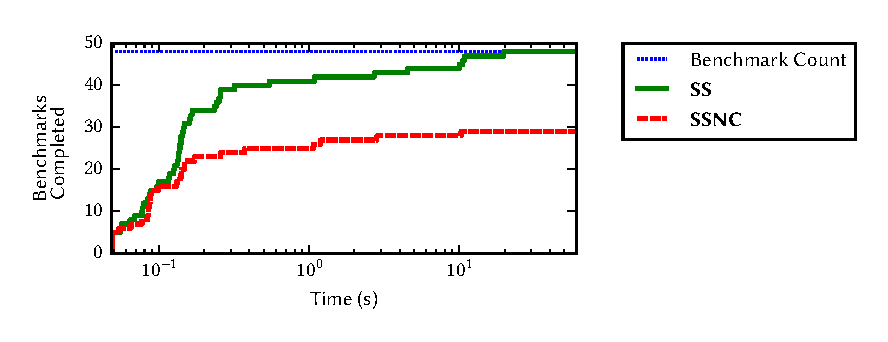
\includegraphics{generated-graphs/times}
  \caption{ Number of benchmarks that can be solved by a given algorithm in a
    given amount of time. \SSOpt{} is the full symmetric synthesis algorithm.
    \BSOpt{} is the full bijective lens synthesis algorithm. \SSNCOpt{} is the
    symmetric synthesis algorithm without using a library of existing lenses.
    \BSNCOpt{} is the bijective synthesis algorithm without using a library of
    existing lenses. Our symmetric synthesis algorithm is able to complete all
    benchmarks in our benchmark suite in under 30 seconds, and is able to
    complete most of the benchmarks without using compositional synthesis. }
  \label{fig:times}
\end{figure}

For each benchmark in our benchmark suite, we ran every mode on it with a
timeout of 30 seconds, and average the result over 5 runs.
Figure~\ref{fig:times} summarizes the results of these tests. We find that our
algorithm is able to synthesize all of the benchmarks in our benchmark suite in
under 30 seconds.

The slowest completed benchmark for both the bijective and symmetric synthesis
algorithms is \texttt{xml\_to\_augeas.boom}, a benchmark that converts
arbitrary XML up to depth 3 into a serialized version of the structured
dictionary representation used in Augeas.  This benchmark takes 18.9 seconds for
the symmetric synthesis algorithm to complete, and 9.3 seconds the bijective
synthesis algorithm to complete.

\subsection{Heuristic Usefulness}
We evaluate the usefulness of (1) our information theoretic metric, and (2) our
termination heuristic.  To this end, we run our program in 3 different modes:\\
\begin{tabulary}{\linewidth}{rL}
  \NoTPOpt{}: & We synthesize lenses using our symmetric synthesis algorithm,
                but users cannot tune when \RXSearch returns using a termination parameter.\\
  \FCOpt{}: &  The first time \GreedySynth finds a lens, it returns that lens.\\
  \NMOpt{}: & \GreedySynth does not have any notion of cost, and searches for
              any lens that satisfies the specification. \\
\end{tabulary}

Figure~\ref{fig:heuristic} summarizes the result of this experiment.  We find
that \afm{TODO}.
% end evaluation

% begin related-work
\section{Related Work}
\label{sec:related}
There is related work in a number of directions. There is related work in
symmetric lenses, string transformation synthesis, and type-directed synthesis.
We also refer the reader to a recent, general survey on synthesis~\ref{?}.

\subsection{Symmetric Lenses}
\paragraph*{Formalization} We have reformulated the problem addressed by
symmetric lenses with simple symmetric lenses. Classically, these types of
synchronization tasks are represented as symmetric lenses. A symmetric lens
$\Lens$ between $X$ and $Y$ consists of 4 components: a complement $C$, a
designated element $init \in C$, and two functions for propagating changes in
each format to the other:
\begin{enumerate}
\item $\PutRSym \OfType X \times C \rightarrow Y \times C$
\item $\PutLSym \OfType Y \times C \rightarrow X \times C$
\end{enumerate}
In this formulation, the components of each format that aren't shared with the
other format are stored in the complement. When one format is edited, the \PutR
or \PutL function stitches together that edited data with the data for the other
side, stored in the complement.  The designated element, $init$, is used as the
initial value of $C$, and specifies default behavior when there isn't existing
data to stitch with.  In our example, the complement would consist of two lists
of commands, where one list contains the Linux commands and one list contains
the Windows commands.

These components only make sense for synchronization when they satisfy
round-tripping laws.  This guarantees that if an identity edit is propagated, no
data gets changed.
\begin{equation}
  \tag{\PutRL}
  \frac{\PutRSymOf{(x,c)} = (y,c'')}{\PutLSymOf{(y,c'')} = (x,c')}
\end{equation}
\begin{equation}
  \tag{\PutLR}
  \frac{\PutLSymOf{(y,c)} = (x,c')}{\PutRSymOf{(x,c')} = (y,c')}
\end{equation}

Furthermore, two symmetric lenses are equivalent if they always output the same
formats on any sequence of edits. Formally, given a lens $\Lens \in X
\leftrightarrow Y$, an \emph{edit} for $\Lens$ is a member of $X + Y$. Consider
the function $apply$, which, given a lens and an element of that lens's
complement, is a function from sequences of edits to sequences of edits. If
$apply(\Lens,c,es) = es'$, then that means, starting with complement $c$, after
edit $es_i$, the lens $\Lens$ synchronizes the other data to $es'_i$.
\[
  \inferrule
  {
  }
  {
    apply(\Lens,c,[]) = []
  }
\]
\[
  \inferrule
  {
    \Lens.putr(x,c) = (y,c')\\
    apply(\Lens,c',es) = es'
  }
  {
    apply(\Lens,c,(\InLOf{x})::es) = (\InROf{y})::es'
  }
\]
\[
  \inferrule
  {
    \Lens.putl(y,c) = (x,c')\\
    apply(\Lens,c',es) = es'
  }
  {
    apply(\Lens,c,(\InROf{y})::es) = (\InLOf{x})::es'
  }
\]

Two lenses, $\Lens_1$ and $\Lens_2$, are equivalent if
$apply(\Lens_1,\Lens_1.init,es) = apply(\Lens_2,\Lens_2.init,es)$ for all edit
sequences $es$.

By describing our lenses in this complement style, we can express an incredibly
wide class of lenses, as these complements permit storing any amount of
information in them.  However, they pose problems when implementing them in
real-world systems and in synthesizing them.

\paragraph*{Issues with Symmetric Lenses} Using symmetric lenses for
synchronization forces us to maintain not just two files that we aim to
sycnrhonize, but three. This is unintuitive, and creates many problems in
practice. For example, consider the situation where I am synchronizing a crontab
and job manager file. I am synchronizing across computers, so I must either
maintain a copy of the complement on each computer, and keep them synchronized,
or figure out a computer to hold the complement, and make sure all edits go
through that complement. Furthermore, if I want to change the synchronization to
a different computer, I don't need to merely make sure that my files are moved
to the computer, I also have to make sure that I correctly move the complement,
and hook up that complement to be used for that synchronization task. This is a
huge divergence from other synchronization utilities, where all that needs to be
done is maintain the files. Using those for synchronization, edits can be sent
over the wire, and the appropriate function can stitch together those edits, no
additional state needed.

For synthesis, because each lens has a custom complement, we can no longer
specify the put functions though mere input/output examples.  Instead, we have
to specify the behavior through the observable behavior of edit sequences.
Furthermore, there are lenses that require arbitrarily long edit sequences to
differentiate between: consider the lens that keeps two formats equal for the
first $k$ non-identity edits, then keeps them completely unsynchronized for all
future edits.  This requires an edit sequence of $k$ edits to differentiate
between this lens and the identity lens.  Simple symmetric lenses avoid this
problem by not allowing such lenses: we can't keep track of the number of
non-identity edits performed unless there are explicit fields in the data
formats keeping track of them.  While we are reducing the expressivity of our
lenses with this restriction, we feel the benefits outweigh the costs.

\paragraph*{Relation with Simple Symmetric Lenses} To formalize how simple
symmetric lenses lenses work as synchronization tools, we define an $apply$
function on them, much like we define an $apply$ on symmetric lenses. The
function $apply$, given a symmetric lens and an optional pair of elements of the
source and target, is a function from sequences of put objects to sequences of
put objects. If $apply(\Lens,\None,es,es')$, then that means, starting with no
prior data, after edit $es_i$, the lens \Lens synchronizes the other data to
$es_i'$. If $apply(\Lens,\SomeOf{(x,y)},es,es')$, then that means, starting with
data $x$ and $y$ on the left and right, respectively, after edit $es_i$, the
lens \Lens synchronizes the other data to $es_i'$.

\[
  \inferrule
  {
  }
  {
    apply(\Lens,xyo,[]) = []
  }
\]
\[
  \inferrule
  {
    \Lens.\CreateROf{x} = y\\
    apply(\Lens,\SomeOf{(x,y)},es) = es'
  }
  {
    apply(l,\None,\InLOf{x}::es) = \InROf{y}::es'
  }
\]
\[
  \inferrule
  {
    \Lens.\CreateLOf{y} = x\\
    apply(\Lens,\SomeOf{(x,y)},es) = es'
  }
  {
    apply(l,\None,\InROf{y}::es) = \InLOf{x}::es'
  }
\]
\[
  \inferrule
  {
    \Lens.\PutROf{x'}{y}  = y'\\
    apply(\Lens,\SomeOf{(x',y')},es) = es'
  }
  {
    apply(l,\SomeOf{(x,y)},\InLOf{x'}::es) = \InROf{y'}::es'
  }
\]
\[
  \inferrule
  {
    \Lens.\PutLOf{y'}{x}  = x'\\
    apply(\Lens,\SomeOf{(x',y')},es) = es'
  }
  {
    apply(l,\SomeOf{(x,y)},\InROf{y'}::es) = \InLOf{x'}::es'
  }
\]

We've reformulated symmetric lenses in a style similar to existing asymmetric
lens formulations. However, some symmetric lenses certainly are inexpressible in
the simple symmetric lens formulation. We formalize which are expressible
with a restriction on symmetric lenses. We define \emph{forgetful symmetric
  lenses} to be symmetric lenses which satisfy the following additional laws:
\begin{equation}
  \tag{\ForgetfulRL}
  \begin{mathprooftree}
    \AxiomC{$\Lens.putr(x,c_1) = (\_,c_1')$}
    \def\extraVskip{.5pt}
    \noLine 
    \UnaryInfC{$\Lens.putr(x,c_2) = (\_,c_2')$}
    \AxiomC{$\Lens.putl(y,c_1') = (\_,c_1'')$}
    \def\extraVskip{.5pt}
    \noLine 
    \UnaryInfC{$\Lens.putl(y,c_2') = (\_,c_2'')$}
    \def\extraVskip{2pt}
    \singleLine
    \BinaryInfC{$c_1'' = c_2''$}
  \end{mathprooftree}
\end{equation}
\begin{equation}
  \tag{\ForgetfulLR}
  \begin{mathprooftree}
    \AxiomC{$\Lens.putl(y,c_1) = (\_,c_1')$}
    \def\extraVskip{.5pt}
    \noLine 
    \UnaryInfC{$\Lens.putl(y,c_2) = (\_,c_2')$}
    \AxiomC{$putr(x,c_1') = (\_,c_1'')$}
    \def\extraVskip{.5pt}
    \noLine 
    \UnaryInfC{$\Lens.putr(x,c_2') = (\_,c_2'')$}
    \def\extraVskip{2pt}
    \singleLine
    \BinaryInfC{$c_1'' = c_2''$}
  \end{mathprooftree}
\end{equation}

Intuitively, this says that the complements are uniquely determined by the most
recently input $x$ and $y$. This corresponds closely with simple symmetric
lenses, where all state is maintained by the current state of the $x$ and $y$
data. Forgetful symmetric lenses express exactly the same $apply$ function as
simple symmetric lenses.

\begin{theorem}
  Let $\Lens$ be a symmetric lens. The lens $\Lens$ is equivalent to a forgetful
  lens if, and only if, there exists a simple symmetric lens $\Lens'$ where
  $apply(\Lens,\Lens.init,es) = apply(\Lens',\None,es)$, for all put sequences $es$.
\end{theorem}

Despite being less expressive than symmetric lenses, simple symmetric lenses are
strictly more expressive than classical asymmetric lenses.

\begin{theorem}
  Let $\Lens$ be an asymmetric lens. $\Lens$ is also a simple symmetric lens,
  where
  \begin{center}
    \begin{tabular}{rcl}
      $\Lens.\CreateROf{x}$ & $=$ & $\Lens.get \App x$\\
      $\Lens.\CreateLOf{y}$ & $=$ & $\Lens.create \App y$\\
      $\Lens.\PutROf{x}{y}$ & $=$ & $\Lens.get \App x$\\
      $\Lens.\PutLOf{y}{x}$ & $=$ & $\Lens.put \App y \App x$
    \end{tabular}
  \end{center}
\end{theorem}

\subsection{String Transformation Synthesis}
Much of the research on string transformation synthesis is on synthesizing
string transformations from input/output
specifications~\cite{flashfill,flashextract,?}. While this provides an easier
interaction model with the user than this work, it requires the algorithm to
learn the data formats from the examples. This makes the task much more
difficult for the synthesis algorithm, particularly in addressing iterations and
disjunctions. Prior work has shown that learning from examples and data format
descriptions enables synthesis of much more complex transformations than are
permitted by examples alone. Recent work has gone into making these algorithms
more robust by delaying the selection of program until seeing what further
inputs the program is run on~\cite{?}. By doing this, the synthesis algorithm
can learn additional information about the formats from the use of the program.

In many of these synthesis algorithms the correct transformation is chosen by
principals like ``minimize constants''~\cite{?,?,?} and ``most specific
generalization''~\cite{?,?,?}. We are the first work to our knowledge to use an
information-theoretic measure for finding the correct transformation. However,
much of our metrics are compatible with existing metrics: avoiding \Disconnect
lenses minimizes constants and creates more specfic transformations (\Disconnect
lenses permit more synchronized data).

Optician~\ref{?} synchronizes string transformation functions, but prior
versions were very restrictive in which transformations were permitted.
Originally, Optician only synchronized transformations between formats in
bijective correspondence, but few formats satisfy that constraint. Recent
enhancements have permitted synthesis of more expressive lenses, quotient
bijective lenses. These enhancements were made by strengthening the
specifications from regular expressions to QREs, regular expressions annotated
with information on normal forms of the language. This enhancement permits
synthesizing transformations between formats whose normal forms are in bijective
correspondence. While we have not integrated our system to permit QRE
specifications, we see no reason the two systems cannot be integrated.

Other work synthesizing invertible transformations was done by inverting a
previously defined transformation.  This has been done by exploiting
parametricity to invert transformations~\cite{?}, and by inverting symbolic
finite automata~\cite{?}.

\subsection{Type-Directed Synthesis}

Type-directed synthesis uses type information to tighten specifications and
reduce the number of possible programs. Typically, type-directed synthesis
techniques use the types to orient the search space.  Our work interestingly
deals with types with many semantic equivalences on them. InSynth~\cite{?}
deals with the same problem when trying to synthesize transformations involving
library functions. InSynth addresses this in a similar manner to this work: by
normalizing the types we don't need to search through the equivalences on those
types.

% end related-work

% begin conclusion
\section{Conclusion}
\label{sec:conc}
We have developed a synthesis algorithm for synthesizing synchronization
functions between data formats that may not be in bijective correspondence. We
do this by synthesizing symmetric lenses. However, existing symmetric lens
formulations use complex complements to store external state. We identify a
restriction on symmetric lenses, simple symmetric lenses. We develop combinators
for simple symmetric lenses on string data. We show how to synthesize these
lenses from regular expression specifications. Prior work could return
\emph{any} satisfying lens, as the type system was restrictive enough that any
satisfying lens would typically be the correct satisfying lens. Because of the
increased flexibility of the symmetric lens language, we identify an
information-theoretic heuristic for finding a likely satisfying lens. We
developed a greedy synthesis algorithm that aims to find the lens of lowest
cost. We demonstrate empiraclly that our algorithm can find lenses quickly, and
our heuristic makes finding the correct lens require fewer specifications.

% end conclusion

% begin acknowledgements
\begin{acks}
\end{acks}
% end acknowledgements

\ifanon\else
\fi

% We recommend abbrvnat bibliography style.

% The bibliography should be embedded for final submission.

\bibliography{local,bcp}

\appendix

\ifappendices

\onecolumn


\paragraph*{Symmetric DNF Lenses: Typing and Semantics}
The typing judgment is a 3-ary relation over a single DNF lens, and two DNF
regular expressions. If $\SDNFLens \OfType \DNFRegex \Leftrightarrow
\DNFRegexAlt$, then the $\SDNFLens.\CreateR$, $\SDNFLens.\CreateL$,
$\SDNFLens.\PutR$, and $\SDNFLens.\PutL$ functions form a symmetric lens.

The typing judgement has 3 components. The first is the sublens components,
confirming that the sequence lenses the DNF lens is comprised of are all
well-typed. The second guarantees that if each sequence on the left has a
sequence lens that can be used for \CreateR{}s and \PutR{}s. The last guarantees
the same for sequences on the right, with \CreateL{} and \PutL{}.

\[
  \inferrule*
  {
    \SSQLens_1 \OfType \Sequence_{i_1} \Leftrightarrow \SequenceAlt_{j_1}\\
    \ldots\\
    \SSQLens_p \OfType \Sequence_{i_p} \Leftrightarrow \SequenceAlt_{j_p}\\\\
    i_{c_1} = 1\\
    \ldots\\
    i_{c_q} = q\\\\
    j_{d_1} = 1\\
    \ldots\\
    j_{d_r} = r
  }
  {
    (\SDNFLensOf{(i_1,j_1,\SSQLens_1)\DNFLSep
      \ldots\DNFLSep
      (i_p,j_p,\SSQLens_p)}
    ,\ListOf{c_1;\ldots;c_q}
    ,\ListOf{d_1;\ldots;d_r})
    \OfType\\\\
    \DNFOf{(\Sequence_1,\Probability_1) \DNFSep \ldots \DNFSep (\Sequence_q,\Probability_q)}
    \Leftrightarrow
    \DNFOf{(\SequenceAlt_1,\ProbabilityAlt_1) \DNFSep \ldots \DNFSep (\SequenceAlt_r,\ProbabilityAlt_q)}
  }
\]

The \CreateR{} function looks for the sequence the provided string matches. If
the string matches sequence $\Sequence_x$, then the lens will look in the create
list at position $x$ to find which sequence lens to use. Then, the sequence lens
transforms the given string using that sequence lens.

The \PutR{} function finds what pairs sequences the input source and view
strings match.  If there that pair of sequences have a sequence lens between
them, then the DNF lens merely performs that sequence lens on the provided
strings.  If there isn't a pair of sequence lenses between them, then \CreateR{}
is performed on the source, with the view forgotten.

The \CreateL{} and \PutL{} functions are defined symmetrically.

\begin{tabular}{@{}r@{\ }c@{\ }l@{}}
  $\CreateR{} \App s$ & = & $\SSQLens_{c_x}.\CreateR{} \App s$ if $s \in \Sequence_x$\\
  $\CreateL{} \App v$ & = & $\SSQLens_{d_y}.\CreateL{} \App v$ if $v \in \SequenceAlt_y$\\
  $\PutR{} \App s \App v$ & = &
                               $\begin{cases*}
                                 \SSQLens_x.\PutR{} \App s \App v & if $s \in \Sequence_{i_x}$ and $v \in \SequenceAlt_{j_x}$\\
                                 \CreateR{} \App s & if $\nexists x.$ $s \in \Sequence_{i_x}$ and $v \in \SequenceAlt_{j_x}$
                               \end{cases*}$\\
  $\PutL{} \App v \App s$ & = &
                               $\begin{cases*}
                                 \SSQLens_y.\PutL{} \App v \App s & if $v \in \SequenceAlt_{j_y}$ and $s \in \Sequence_{i_y}$\\
                                 \CreateL{} \App v & if $\nexists y.$ $v \in \SequenceAlt_{j_y}$ and $s \in \Sequence_{i_y}$
                               \end{cases*}$
\end{tabular}

\paragraph*{Symmetric Sequence Lenses: Typing and Semantics}
The typing judgment is a 3-ary relation over a single Sequence lens, and two
sequences. If $\SSQLens \OfType \Sequence \Leftrightarrow \SequenceAlt$, then
the $\SSQLens.\CreateR$, $\SSQLens.\CreateL$, $\SSQLens.\PutR$, and
$\SSQLens.\PutL$ functions form a symmetric lens.

The typing judgement has 4 components. The first is the sublens components,
confirming that the atom lenses the sequence lens is comprised of all are
well-typed. The second guarantees that if each string that will be used for
\CreateR{}s are members of the correct atoms.  The third guarantees
the same for strings and atoms on the right, with \CreateL.  The last guarantees
that each atom is mapped by at most one atom lens.

\[
  \inferrule*
  {
    \SAtomLens_1 \OfType \Atom_{i_1} \Leftrightarrow \AtomAlt_{j_1}\\
    \ldots\\
    \SAtomLens_p \OfType \Atom_{i_p} \Leftrightarrow \AtomAlt_{j_p}\\\\
    \String_1 \in \Atom_1\\
    \ldots\\
    \String_q \in \Atom_q\\\\
    \StringAlt_1 \in \AtomAlt_1\\
    \ldots\\
    \StringAlt_r \in \AtomAlt_r\\\\
    i_x = i_y \BooleanImplies x = y\\
    j_x = j_y \BooleanImplies x = y
  }
  {
    (\SSQLensOf{(i_1,j_1,\SAtomLens_1)\SeqLSep
      \ldots\SeqLSep
      (i_p,j_p,\SAtomLens_p)}
    ,\ListOf{\String_1;\ldots;\String_q}
    ,\ListOf{\StringAlt_1;\ldots;\StringAlt_r})\\
    \OfType
    \SequenceOf{\String_0'''' \SeqSep \Atom_1 \SeqSep \ldots \SeqSep \Atom_q
      \SeqSep \String_q'}
    \Leftrightarrow
    \SequenceOf{\StringAlt_0' \SeqSep \AtomAlt_1 \SeqSep \ldots \SeqSep \AtomAlt_r \SeqSep \StringAlt_r'}
  }
\]

For each component of the string matching an atom, the \CreateR function looks
for the atom lens that maps on the atom. If there is such an atom lens,
\SAtomLens, then that the sequence lens puts the provided string into the
default string for the target atom. If there is no such atom lens, then the
sequence lens merely uses the default string.

For each component of the string matching an atom, the \PutR function looks
for the atom lens that maps on the atom. If there is such an atom lens,
\SAtomLens, then that the atom lens puts the provided string of the source atom into the
string of the target atom. If there is no such atom lens, then the
sequence lens merely recovers the target's string.

The \CreateL{} and \PutL{} functions are defined symmetrically.

\begin{tabular}{@{}r@{\ }c@{\ }l@{}}
  $\CreateR{} \App \String_0'\Concat \String_1'' \Concat \ldots \Concat \String_q'' \Concat \String_q'$
  & = 
  & $\StringAlt_0' \Concat \StringAlt_1'' \Concat \ldots \Concat
    \StringAlt_r'' \Concat \StringAlt_r'$\\
  & & where $\StringAlt_y'' =
    \begin{cases*}
      \SAtomLens_k.\PutROf{\String_{i_k}''}{\StringAlt_y} & if $j_k = y$\\
      \StringAlt_y & if $\nexists k. j_k = y$\\
    \end{cases*}$\\
  $\CreateL{} \App \StringAlt_0'\Concat \StringAlt_1'' \Concat \ldots \Concat \StringAlt_q''
  \Concat \StringAlt_q'$
  & = 
  & $\String_0' \Concat \String_1'' \Concat \ldots \Concat
    \String_r'' \Concat \String_r'$\\
  & & where $\String_x'' =
    \begin{cases*}
      \SAtomLens_k.\PutROf{\StringAlt_{j_k}''}{\String_x} & if $i_k = x$\\
      \String_x & if $\nexists k. i_k = x$\\
    \end{cases*}$\\
  $\PutR{} \App (\String_0'\Concat \String_1'' \Concat \ldots \Concat \String_q'' \Concat \String_q') \App (\StringAlt_0'\Concat \StringAlt_1'' \Concat \ldots \Concat \StringAlt_q'' \Concat \StringAlt_q')$
  & =
  & $\StringAlt_0'\Concat \StringAlt_1''' \Concat \ldots \Concat \StringAlt_q''' \Concat \StringAlt_q'$\\
  & & where
      $t_y''' =
      \begin{cases*}
        \SAtomLens_k.\PutROf{\String_{i_k}''}{\StringAlt_{y}''} & if $j_k = y$\\
        \StringAlt_y'' & if $\nexists k. j_k = y$\\
      \end{cases*}$\\
  $\PutL{} \App (\StringAlt_0'\Concat \StringAlt_1'' \Concat \ldots \Concat \StringAlt_q'') \Concat (\StringAlt_q' \App \String_0'\Concat \String_1'' \Concat \ldots \Concat \String_q'' \Concat \String_q')$
  & =
  & $\String_0'\Concat \String_1''' \Concat \ldots \Concat \String_r''' \Concat \String_r'$\\
  & & where
      $s_x''' =
      \begin{cases*}
        \SAtomLens_k.\PutLOf{\StringAlt_{j_k}''}{\String_{x}''} & if $i_k = x$\\
        \String_x'' & if $\nexists k. i_k = x$\\
      \end{cases*}$\\
\end{tabular}

\paragraph*{Symmetric Atom Lenses: Typing and Semantics}
The typing judgment is a 3-ary relation over a single atom lens, and two
atoms. If $\SAtomLens \OfType \Atom \Leftrightarrow \AtomAlt$, then
the $\SAtomLens.\CreateR$, $\SAtomLens.\CreateL$, $\SAtomLens.\PutR$, and
$\SAtomLens.\PutL$ functions form a symmetric lens.

The typing judgement just confirms that the DNF lens that comprises the
sequence lens is also well typed.

\[
  \inferrule*
  {
    \SDNFLens \OfType \DNFRegex \Leftrightarrow \DNFRegexAlt
  }
  {
    \StarOf{\SDNFLens}
    \OfType \PRegexStar{\DNFRegex}{\Probability}
    \Leftrightarrow \PRegexStar{\DNFRegexAlt}{\ProbabilityAlt}
  }
\]

For each component of the string matching an atom, the \CreateR function looks
for the atom lens that maps on the atom. If there is such an atom lens,
\SAtomLens, then that the sequence lens puts the provided string into the
default string for the target atom. If there is no such atom lens, then the
sequence lens merely uses the default string.

For each component of the string matching an atom, the \PutR function looks
for the atom lens that maps on the atom. If there is such an atom lens,
\SAtomLens, then that the atom lens puts the provided string of the source atom into the
string of the target atom. If there is no such atom lens, then the
sequence lens merely recovers the target's string.

The \CreateL{} and \PutL{} functions are defined symmetrically.

\begin{tabular}{@{}r@{\ }c@{\ }l@{}}
  $\CreateR{} \App \String_0 \Concat \ldots \Concat \String_n$
  & = 
  & $\StringAlt_1 \Concat \ldots \Concat \StringAlt_n$
  where $\StringAlt_i = \SDNFLens.\CreateR \App \String_i$\\
  $\CreateL{} \App \StringAlt_0 \Concat \ldots \Concat \StringAlt_m$
  & = 
  & $\String_1 \Concat \ldots \Concat \String_m$
  where $\String_i = \SDNFLens.\CreateL \App \StringAlt_i$\\
  $\PutR{} \App (\String_0 \Concat \ldots \Concat \String_n) \App
  (\StringAlt_1 \Concat \ldots \Concat \StringAlt_m)$
  & = 
  & $\StringAlt_1' \Concat \ldots \Concat \StringAlt_n'$
    where $\StringAlt_i' =
    \begin{cases*}
      \SDNFLens.\PutR \App \String_i \App \StringAlt_i & if $i \leq m$\\
      \SDNFLens.\CreateR \App \String_i & otherwise
    \end{cases*}$\\
  $\PutL{} \App (\StringAlt_1 \Concat \ldots \Concat \StringAlt_m) \App
  (\String_0 \Concat \ldots \Concat \String_n)$
  & = 
  & $\String_1' \Concat \ldots \Concat \String_m'$
    where $\String_i' =
    \begin{cases*}
      \SDNFLens.\PutL \App \StringAlt_i \App \String_i & if $i \leq n$\\
      \SDNFLens.\CreateL \App \StringAlt_i & otherwise
    \end{cases*}$\\
\end{tabular}


\section{Forgetful Symmetric Lenses}

\begin{property}[Starting Forgetfulness RL]
  \label{prop:forget-rl}
  Let $\Lens$ be a forgetful symmetric lens.  If $(x_1',c_1') = \Lens.\PutL \App
  (y,\Snd \App (\Lens.\PutR \App (x,c_1)))$, and
  $(x_2',c_2') = \Lens.\PutL \App
  (y,\Snd \App (\Lens.\PutR \App (x,c_2)))$, then $x_1' = x_2'$.
\end{property}
\begin{proof}
  By \ForgetfulRL, $c_1' = c_2'$. We know $(y,c_1') = \Lens.\PutR \App
  (x_1',c_1')$ and $(y,c_1') = \Lens.\PutR \App (x_2',c_1')$ by \PutLR. By
  \PutRL, we know $(x_1' = \Lens.\PutL \App (y,c_1'))$ and $(x_2' = \Lens.\PutL
  \App (y,c_1')))$. Therefore, by transitivity of equality, $x_1' = x_2'$.
\end{proof}

\begin{property}[Starting Forgetfulness LR]
  \label{prop:forget-lr}
  Let $\Lens$ be a forgetful symmetric lens.  If $(y_1',c_1') = \Lens.\PutR \App
  (x,\Snd \App (\Lens.\PutL \App (y,c_1)))$, and
  $(x_2',c_2') = \Lens.\PutL \App
  (x,\Snd \App (\Lens.\PutR \App (y,c_2)))$,
  then $x_1' = x_2'$.
\end{property}
\begin{proof}
  Symmetric to Starting Forgetfulness RL.
\end{proof}

\begin{definition}[S]
  Let $\Lens$ be a forgetful lens.

  Consider the following four functions $S(\Lens)$, that we wish to satisfy the
  simple symmetric lens laws.

  \begin{centering}
    \begin{tabular}{@{}r@{\ }c@{\ }l@{}}
      $\CreateR{} \App s$
      & =
      & $\Fst \App (\Lens.\PutR{} \App (s,\Lens.init))$\\
      
      $\CreateL{} \App v$
      & =
      & $\Fst \App (\Lens.\PutL{} \App (v,\Lens.init))$\\
      
      $\PutR{} \App s \App v$
      & =
      & $\LetIn{(\_,c)}{\Lens.\PutL \App (v,\Lens.init)}$\\
      &
      & $\LetIn{(s',\_)}{\Lens.\PutR \App (s,c)}$\\
      &
      & $s'$\\
      
      $\PutL{} \App v \App s$
      & =
      & $\LetIn{(\_,c)}{\Lens.\PutR \App (s,\Lens.init)}$\\
      &
      & $\LetIn{(y',\_)}{\Lens.\PutL \App (v,c)}$\\
      &
      & $y'$\\
    \end{tabular}
  \end{centering}
\end{definition}

\begin{mylemma}
  If $\Lens$ is a forgetful symmetric lens, then $S(\Lens)$ is a simple symmetric
  lens.
\end{mylemma}
\begin{proof}
  
  \CreatePutRL{}:
  
  \begin{centering}
    \begin{tabular}{@{}r@{\ }c@{\ }l@{\ }l}
      $S(\Lens).\PutLOf{(S(\Lens).\CreateROf{x})}{x}$
      & =
      & $S(\Lens).\PutLOf{(\Fst \App (\Lens.\PutR{(x,\Lens.init)}))}{x}$
      & By unfolding definitions
      \\
      
      & =
      & $\LetIn{(\_,c)}{\Lens.\PutR \App (x,\Lens.init)}$\\
      &
      & $\LetIn{(y',\_)}{\Lens.\PutL \App (\Fst \App (\Lens.\PutR{(x,\Lens.init)}),c)}$\\
      &
      & $y'$
      & By unfolding definitions\\
      
      & =
      & $\LetIn{(y',\_)}{\Lens.\PutL \App (\Lens.\PutR \App (x,\Lens.init))}$\\
      &
      & $y'$
      & By tuple harmony \\
      
      & =
      & $x$
      & By \PutRL \\
    \end{tabular}
  \end{centering}

  \CreatePutLR{}:  Symmetric to \CreatePutRL{}

  \PutRL{}:

  \begin{centering}
    \begin{tabular}{@{}r@{\ }c@{\ }l@{\ }l}
      $S(\Lens).\PutLOf{(S(\Lens).\PutROf{x}{y})}{x}$
      & =
      & $\LetIn{(\_,c)}{\Lens.\PutL \App (y,\Lens.init)}$\\
      & & $\LetIn{(y',c')}{\Lens.\PutR \App (x,c)}$\\
      & & $S(\Lens).\PutLOf{y'}{x}$
      & By unfolding definitions
      \\
      
      & =
      & $\LetIn{(\_,c)}{\Lens.\PutL \App (y,\Lens.init)}$\\
      & & $\LetIn{(y',c')}{\Lens.\PutR \App (x,c)}$\\
      & & $\LetIn{(\_,c'')}{\Lens.\PutR \App (x,\Lens.init)}$\\
      & & $\LetIn{(x',c''')}{\Lens.\PutL \App (y',c'')}$\\
      & & $x'$
      & By unfolding definitions
    \end{tabular}
  \end{centering}

  At this point, we know from \PutRL that $(x,c') = \Lens.\PutL \App (y',c')$.
  By Property~\ref{prop:forget-rl}, this means that $x' = x$, as desired.

  \PutLR{}:  Symmetric to \PutRL{}
\end{proof}

\begin{definition}
  Fix a symmetric lens $\Lens$ beteween $X$ and $Y$. Consider the
  function, $\SingleApp_{\Lens} \OfType (X + Y) \times \Lens.C
  \rightarrow ((X + Y) \times \Lens.C)$, defined as:

  \begin{tabular}{@{}r@{\ }c@{\ }l@{\ }l}
    $\SingleApp_{\Lens}(\InLOf{x},c)$
    & =
    & $\LetIn{(y,c')}{\Lens.\PutRSymOf{(x,c)}}$\\
    &
    & $(\InROf{y},c')$\\
    
    $\SingleApp_{\Lens}(\InROf{y},c)$
    & =
    & $\LetIn{(x,c')}{\Lens.\PutLSymOf{(y,c)}}$\\
    &
    & $(\InLOf{x},\SomeOf{(x,y)})$
  \end{tabular}
\end{definition}

\begin{definition}
  Fix a simple symmetric lens $\Lens$ beteween $X$ and $Y$. Consider the
  function, $\SingleApp_{\Lens} \OfType ((X + Y) \times \OptionOf{(X \times Y)})
  \rightarrow ((X + Y) \times \OptionOf{(X \times Y)})$, defined as:

  \begin{tabular}{@{}r@{\ }c@{\ }l@{\ }l}
    $\SingleApp_{\Lens}(\InLOf{x},\None)$
    & =
    & $\LetIn{y}{\Lens.\CreateROf{x}}$\\
    &
    & $(\InROf{y},\SomeOf{(x,y)})$\\
    
    $\SingleApp_{\Lens}(\InROf{y},\None)$
    & =
    & $\LetIn{x}{\Lens.\CreateLOf{y}}$\\
    &
    & $(\InLOf{x},\SomeOf{(x,y)})$\\
    
    $\SingleApp_{\Lens}(\InLOf{x'},\SomeOf{(x,y)})$
    & =
    & $\LetIn{y'}{\Lens.\PutROf{x'}{y}}$\\
    &
    & $(\InROf{y'},\SomeOf{(x',y')})$\\
    
    $\SingleApp_{\Lens}(\InROf{y'},\SomeOf{(x,y)})$
    & =
    & $\LetIn{x'}{\Lens.\PutLOf{y'}{x}}$\\
    &
    & $(\InROf{x'},\SomeOf{(x',y')})$\\
  \end{tabular}
\end{definition}

\begin{definition}
  Fix a symmetric lens \Lens over $X$ and $Y$. We define the relation $R_\Lens$
  over $\Lens.C$ and $\OptionOf{(X \times Y)}$ as the largest relation such
  that:
  \begin{enumerate}
  \item $R_\Lens(c,None) \BooleanImplies c = \Lens.init$
  \item $R_\Lens(c,Some (x,y)) \BooleanImplies
    \Lens.\PutRSymOf{(x,c)} = (y,c) \BooleanAnd
    \Lens.\PutLSymOf{(y,c)} = (x,c)$
  \end{enumerate}
\end{definition}

\begin{mylemma}
  \label{lem:s-equiv}
  Let $\Lens$ be a symmetric lens.  Let $c \in \Lens.C$ be a complement, and
  $xyo \in \OptionOf{(X \times Y)}$.  If $R_{\Lens}(c,xyo)$, then
  $apply(\Lens,c,es) = apply(S(\Lens),xyo,es)$.
\end{mylemma}
\begin{proof}
  By induction on the derivation the application of $apply(S(\Lens),xyo,es)$
  \begin{case}[empty list]
    So by the case, $apply(S(\Lens),xyo,[]) = []$. Furthermore,
    $apply(\Lens,c,[]) = []$, as desired.
  \end{case}
  \begin{case}[first edit is a create right]
    So by the case, $apply(S(l),\None,\InLOf{x}::es) = \InROf{y}::es'$, where
    $S(\Lens).\CreateROf{x} = y$ and $apply(S(\Lens),\SomeOf{(x,y)},es) = es'$.

    As $R_{\Lens}(None,c)$, $c = \Lens.init$. So, performing $apply$ on
    $\Lens.init$, we get $apply(\Lens,\Lens.init,(\InLOf{x})::es) =
    (\InROf{y'})::es''$ where $\Lens.putr(x,c) = (y',c')$ and $apply(\Lens,c',es)
    = es'$.

    So, by definition, $S(\Lens).\CreateROf{x} = \Fst \App (\Lens.\PutRSymOf{(x,\Lens.init)})$, so $y = y'$.

    Furthermore, by \PutRL, $\Lens.\PutLSymOf{(y,c')} = (x,c')$, and by another
    application of \PutLR, $\Lens.\PutRSymOf{(x,c')} = (y,c')$.  This means
    that $R_{\Lens}(c',Some (x,y))$.

    So, by induction assumption, $apply(\Lens,c',es) = apply(S(\Lens),xyo,es)$, so
    $es' = es''$.  This means, $apply(S(l),\None,\InLOf{x}::es) =
    \InROf{y}::es'$ and $apply(\Lens,\Lens.init,(\InLOf{x})::es) =
    (\InROf{y})::es'$, so they are equal, as desired.
  \end{case}
  \begin{case}[first edit is a create left]
    Symmetric to previous case
  \end{case}
  \begin{case}[first edit is a put right]
    So by the case, $apply(S(\Lens),\SomeOf{(x,y)},\InLOf{x'}::es) = \InROf{y'}::es'$, where
    $S(\Lens).\PutROf{x}{y} = y'$ and $apply(S(\Lens),\SomeOf{(x',y')},es) = es'$.

    Performing $apply$ on $c$, we get $apply(\Lens,c,(\InLOf{x'})::es) =
    (\InROf{y'})::es''$ where $\Lens.\PutRSymOf{(x',c)} = (y',c')$ and
    $apply(\Lens,c',es) = es''$.

    So, by definition, $S(\Lens).\PutROf{x}{y} = \Fst \App (\Lens.\PutRSymOf{(x,c'')})$, where $c'' = \Snd \App (\Lens.\PutLSymOf{(y,\Lens.init)})$.

    By assumption, $R_{\Lens}(c,\SomeOf{(x,y)})$, so $\Lens.\PutLSymOf{(y,c)}
    = (x,c)$.  So, by Property~\ref{prop:forget-lr}, we know $y' = y''$.

    Furthermore, by \PutRL, $\Lens.\PutLSymOf{(y',c')} = (x',c')$, and by another
    application of \PutLR, $\Lens.\PutRSymOf{(x',c')} = (y',c')$.  This means
    that $R_{\Lens}(c',Some (x',y'))$.

    So, by induction assumption, $apply(\Lens,c',es) = apply(S(\Lens),xyo,es)$, so
    $es' = es''$.  This means, $apply(S(l),\SomeOf{(x,y)},\InLOf{x'}::es) =
    \InROf{y'}::es'$ and $apply(\Lens,c,(\InLOf{x'})::es) =
    (\InROf{y'})::es'$, so they are equal, as desired.
  \end{case}
  \begin{case}[first edit is a put left]
    Symmetric to previous case
  \end{case}
\end{proof}

\begin{definition}[F]
  Let $\Lens$ be a simple symmetric lens between $X$ and $Y$.

  Consider the following set $C$, distinguished element of that set, $init$, and
  pair of functions $\PutRSym$ and $\PutLSym$, that we wish to satisfy the
  symmetric lens laws, and that we also wish to be forgetful.

  \begin{centering}
    \begin{tabular}{@{}r@{\ }c@{\ }l@{}}
      $C$
      & =
      & $\OptionOf{(X \times Y)}$\\
      
      $init$
      & =
      & $\None$\\
      
      $\PutRSymOf{(x,c)}$
      & =
      & $(y,\SomeOf{(x,y)})$ where $y = \begin{cases*}
        \Lens.\CreateROf{x} & if $c = \None$\\
        \Lens.\PutROf{x}{y'} & if $c = \SomeOf{(x',y')}$\\
        \end{cases*}$\\
      
      $\PutLSymOf{(y,c)}$
      & =
      & $(x,\SomeOf{(x,y)})$ where $x = \begin{cases*}
        \Lens.\CreateLOf{y} & if $c = \None$\\
        \Lens.\PutLOf{y}{x'} & if $c = \Some{(x',y')}$\\
        \end{cases*}$\\
    \end{tabular}
  \end{centering}
\end{definition}

\begin{mylemma}
  \label{lem:f-sym}
  If $\Lens$ is a simple symmetric lens, then $F(\Lens)$ is a symmetric lens.
\end{mylemma}
\begin{proof}
  \PutRL: There are two cases, $c = \None$, and $c = \SomeOf{(x,y)}$.

  \begin{case}[c = \None]
    Let $(y',c') = F(\Lens).\PutRSymOf{(x',\None)}$. This means that $y' =
    \Lens.\CreateROf{x'}$, and $c' = \SomeOf{(x',y')}$.
    
    Now, consider $(x'',c'') = F(\Lens).\PutLSymOf{(y',\SomeOf{(x',y')})}$. By
    unfolding definitions, $x'' = \Lens.\PutLOf{y'}{x'}$. By \CreatePutRL, $x''
    = x'$, meaning $c'' = \SomeOf{(x',y')}$. This means $(x',c') =
    F(\Lens).\PutLSymOf{(y',\SomeOf{(x',y')})}$, as desired.
  \end{case}

  \begin{case}[c = \SomeOf{(x,y)}]
    Let $(y',c') = F(\Lens).\PutRSymOf{(x',\SomeOf{(x,y)})}$. This means that $y' =
    \Lens.\PutROf{x'}{y}$, and $c' = \SomeOf{(x',y')}$.
    
    Now, consider $(x'',c'') = F(\Lens).\PutLSymOf{(y',\SomeOf{(x',y')})}$. By
    unfolding definitions, $x'' = \Lens.\PutLOf{y'}{x'}$. By \PutRL, $x''
    = x'$, meaning $c'' = \SomeOf{(x',y')}$. This means $(x',c') =
    F(\Lens).\PutLSymOf{(y',\SomeOf{(x',y')})}$, as desired.
  \end{case}

  The second requirement, \PutLR, is symmetric.
\end{proof}


\begin{mylemma}
  If $\Lens$ is a simple symmetric lens, then $F(\Lens)$ is a forgetful symmetric lens.
\end{mylemma}
\begin{proof}
  By Lemma~\ref{lem:f-sym}, we know $F(\Lens)$ is symmetric, so we merely need
  to show it is forgetful.  We will tackle merely \ForgetfulRL, as the proof for
  \ForgetfulLR is symmetric.

  Let $c_1$ and $c_2$ be two arbitrary complements, and $x$ and $y$ two
  arbitrary values of $X$ and $Y$, respectively.
  
  We know that $c_1' = \Snd \App (F(\Lens).\PutRSymOf{(x,c_1)})$ and $c_2' =
  \Snd \App (F(\Lens).\PutRSymOf{(x,c_2)})$.  Now, by inversion on
  $F(\Lens).\PutRSym$, we know that both $c_1' = Some(x,y_1')$ and $c_2' =
  Some(x,y_2')$ for some values of $y_1$ and $y_2$ (though we don't actually
  care about the values of $y_1$ and $y_2$).

  Now by unfolding definitions we know, $\Snd \App
  (F(\Lens).\PutLSymOf{(y,\SomeOf{(x,y_1')})}) =
  \SomeOf(\Lens.\PutLOf{x}{y},y) = c_1''$. Similarly, we know $\Snd \App
  (F(\Lens).\PutLSymOf{(y,\SomeOf{(x,y_2')})}) =
  \SomeOf(\Lens.\PutLOf{x}{y},y) = c_2''$, so $c_1'' = c_2''$, as intended.
\end{proof}

\begin{mylemma}
\label{lem:f-equiv}
  If $\Lens$ be a simple symmetric lens, then $apply(\Lens,xyo,es) =
  apply(F(\Lens),xyo,es)$.
\end{mylemma}
\begin{proof}
  By induction on the derivation of $apply$ on $\Lens$!

  \begin{case}[empty list]
    So by the case, $apply(S(\Lens),xyo,[]) = []$. Furthermore,
    $apply(\Lens,xyo,[]) = []$, as desired.
  \end{case}

  \begin{case}[first edit is a create right]
    So by the case, $apply(\Lens,\None,\InLOf{x}::es) = \InROf{y}::es'$, where
    $\Lens.\CreateROf{x} = y$ and $apply(\Lens,\SomeOf{(x,y)},es) = es'$.

    Performing $apply$ on
    $\None$, we get $apply(F(\Lens),\None,(\InLOf{x})::es) =
    (\InROf{y'})::es''$ where $F(\Lens).putr(x,\None) = (y',c)$ and $apply(\Lens,c,es)
    = es'$.

    Unfolding definitions, $F(\Lens).putr(x,\None) = \Lens.\CreateROf{x} =
    (y,\SomeOf{(x,y)})$, so $c = \SomeOf{(x,y)}$ and $y = y'$

    So, by induction assumption, $apply(\Lens,\SomeOf{(x,y)},es) = apply(F(\Lens),\SomeOf{(x,y)},es)$, so
    $es' = es''$.  This means, $apply(\Lens,\None,\InLOf{x}::es) =
    \InROf{y}::es'$ and $apply(F(\Lens),\None,(\InLOf{x})::es) =
    (\InROf{y})::es'$, so they are equal, as desired.
  \end{case}

  \begin{case}[first edit is a create left]
    Symmetric to previous case
  \end{case}

  \begin{case}[first edit is a put right]
    So by the case, $apply(\Lens,\SomeOf{(x,y)},\InLOf{x'}::es) = \InROf{y'}::es'$, where
    $\Lens.\PutROf{x}{y} = y'$ and $apply(\Lens,\SomeOf{(x',y')},es) = es'$.

    Performing $apply$ on $F(\Lens)$, we get
    $apply(F(\Lens),\SomeOf{(x,y)},(\InLOf{x'})::es) = (\InROf{y'})::es''$ where
    $F(\Lens).\PutRSymOf{(x',\SomeOf{(x,y)})} = (y'',\SomeOf{(x',y'')})$ and
    $apply(\Lens,c',es) = es''$.
    
    So, by definition, $\Fst \App (F(\Lens).\PutRSymOf{(x',\SomeOf{(x,y)})})
    = \Lens.PutROf{x'}{y'}$, so also by definition, $c' = \SomeOf{(x',y')}$.

    So, by induction assumption, $apply(\Lens,\SomeOf{(x',y')},es) =
    apply(F(\Lens),\SomeOf{(x',y')},es)$, so $es' = es''$. This means,
    $apply(\Lens,\SomeOf{(x,y)},\InLOf{x'}::es) = \InROf{y'}::es'$ and
    $apply(F(\Lens),\SomeOf{(x,y)},(\InLOf{x'})::es) = (\InROf{y'})::es'$, so
    they are equal, as desired.
  \end{case}

  \begin{case}[first edit is a put left]
    Symmetric to previous case
  \end{case}
\end{proof}

\begin{theorem}
  Let $\Lens$ be a symmetric lens. The lens $\Lens$ is equivalent to a forgetful
  lens if, and only if, there exists a simple symmetric lens $\Lens'$ where
  $apply(\Lens,\Lens.init,es) = apply(\Lens',\None,es)$, for all put sequences
  $es$.
\end{theorem}

\begin{proof}
  \begin{case}[$\Rightarrow$]
    Let $\Lens$ be equivalent to a forgetful lens $\Lens'$.  Consider the
    simple symmetric lens, $S(\Lens')$.  By Lemma~\ref{lem:s-equiv},
    $apply(\Lens',\Lens'.init,es) = apply(S(\Lens'),\None,es)$.  As $\Lens$ is
    equivalent to $\Lens'$, $apply(\Lens,\Lens.init,es) =
    apply(\Lens',\Lens'.init,es)$.  So, by transitivity,
    $apply(\Lens,\Lens.init,es) = apply(S(\Lens),\None,es)$.
  \end{case}

  \begin{case}[$\Leftarrow$]
    Let $\Lens'$ be a simple symmetric lens where $apply(\Lens,\Lens.init,es) =
    apply(\Lens',\None,es)$, for all put sequences $es$.

    Consider $F(\Lens')$, a forgetful symmetric lens where $apply(\Lens',\None,es) =
    apply(F(\Lens'),\Lens'.init,es)$, for all put sequences $es$, as
    $\Lens'.init = \None$, by Lemma~\ref{lem:f-equiv}.  By transitivity, $apply(\Lens,\Lens.init,es) =
    apply(\Lens',\Lens'.init,es)$, so $\Lens$ and $\Lens'$ are equivalent.
  \end{case}
    
\end{proof}

\fi
\section{Forgetful Symmetric Lenses}
\begin{theorem*}
  If $\Regex \SSREquiv \RegexAlt$ then $\ProbabilityOf{\Regex}{\String} =
  \ProbabilityOf{\RegexAlt}{\String}$, for all strings $\String \in \LanguageOf{\Regex}$.
\end{theorem*}
The following lemma is
\begin{proof}
\begin{enumerate}

\item
($S \; |_1 \; \varnothing \equiv^S S$)

For all $s \in \mathcal{L}(S \; | \; \varnothing)$, then $P_{S \; |_1 \; \varnothing} = 1 * P_S(s) = P_S(s)$.
\item
($S \cdot \varnothing \equiv^S \varnothing$)

For all $s \in \mathcal{L}(S \cdot \varnothing)$, the $P_{S \cdot \varnothing}(s) = \sum_{s_1 \cdot s_2}P_S(s_1) * P_{\varnothing}(s_2)$, but this sum is empty, hence $P_{S \cdot \varnothing}(s) = 0 = P_{\varnothing}(s)$.
\item
($\varnothing \cdot S \equiv^S \varnothing$)

Similar to the previous case.
\item
($(S \cdot S') \cdot S'' \equiv^S S \cdot (S' \cdot S'')$). Let $s \in \mathcal{L}(S \cdot S' \cdot S'')$

Then
\begin{align*}
P_{(S \cdot S') \cdot S''}(s) &= \sum_{s=s_4 \cdot s_3}P_{S \cdot S'}(s_4) * P_{S''}(s_3)\\
&= \sum_{s=s_4 \cdot s_3}\left(\sum_{s_4=s_1 \cdot s_2} P_{S}(s_1) * P_{S'}(s_2)\right)* P_{S''}(s_3)\\
&= \sum_{s=s_1\cdot s_2 \cdot s_3} P_{S}(s_1) * P_{S'}(s_2) * P_{S''}(s_3)\\
P_{S \cdot (S' \cdot S'')}(s) &= \sum_{s=s_1\cdot s_4} P_{S}(s) * \left(\sum_{s_4=s_2\cdot s_3}P_{S'}(s_2) * P_{S''}(s_3)\right)
\end{align*}
\item
($(S \; |_{p_1} \; S') \; |_{p_2} \; S'' \equiv^S S \; |_{p_1 * p_2} \; (S' \; |_{\frac{(1-p_1)*p_2}{1-p_1*p_2}} \; S'')$)

Let $s \in \mathcal{L}(S \; |\; S' \; | \; S'')$. Then
\begin{align*}
P_{(S \; |_{p_1} \; S') \; |_{p_2} \; S''}(s) &= p_2 * P_{S \; |_{p_1} \; S'}(s) + (1-p_2)P_{S''}(s)\\
&= (p_2 * (p_1 * P_S(s) + (1-p_1) * P_{S'}(s))) + (1-p_2)P_{S''}(s)\\
&= (p_2 * (p_1 * P_S(s) + P_{S'}(s)-p_1* P_{S'}(s))) + (1-p_2)P_{S''}(s)\\
&= p_2*p_1 * P_S(s) + p_2*P_{S'}(s)-p_2*p_1* P_{S'}(s) + (1-p_2)P_{S''}(s)\\
&= p_2*p_1 * P_S(s) + (1-p_1) * p_2 * P_{S'}(s)+ (1-p_2)P_{S''}(s)\\
S \; |_{p_1 * p_2} \; (S' \; |_{\frac{(1-p_1)*p_2}{1-p_1*p_2}} \; S'') &= (p_1p_2)  P_S(s) + (1-p_1p_2)  \left(\frac{(1-p_1)p_2}{1-p_1p_2}  P_{S'}(s) + \left(1-\frac{(1-p_1)p_2}{1-p_1p_2}\right)P_{S''}(s)\right)
\end{align*}
\item
($S \; |_p \; T \equiv^S T \; |_{1-p} \; S$)

For all $s \in \mathcal{L}(S \; | \; T)$, we have
$$P_{S \; |_p \; T}(s) = p*P_S(s) + (1-p)*P_T(s) = (1-p) * P_T(s) + (1-(1-p))*P_s(s) = P_{T \; |_{1-p} \; S}(s)$$
\item
($S \cdot (S' \; |_p \; S'' ) \equiv^S (S \cdot S') \; |_p \; (S \cdot S'')$)

For all $s \in \mathcal{L}(S \cdot (S' \sep S''))$ we have
\begin{align*}
P_{S \cdot (S' \; |_p \; S'' )} &= \sum_{s_1 \cdot s_2 = s}P_S(s_1) * P_{S' \; |_p \; S''}(s)\\
&= \sum_{s_1 \cdot s_2 = s}P_S(s_1) * (p * P_{S'}(s_2) + (1-p) * P_{S''}(s_2))\\
&= \sum_{s_1 \cdot s_2 = s}p * P_S(s_1) * P_{S'}(s_2) + \sum_{s_1 \cdot s_2 = s}(1-p) * P_S(s_1) * P_{S''}(s_2)\\
P_{(S \cdot S') \; |_p \; (S \cdot S'')}(s) &= p*P_{S \cdot S'}(s) + (1-p)*P_{S \cdot S''}(s)
\end{align*}
\item
$((S' \; |_p \; S'') \cdot S \equiv^S (S' \cdot S) \; |_p \; (S'' \cdot S))$

For all $s \in \mathcal{L}((S' \; | \; S'') \cdot S)$,  we have
\begin{align*}
P_{(S' \; |_p \; S'') \cdot S}(s) &= \sum_{s_1 \cdot s_2 = s}P_{S' \; |_p \; S''}(s_1) * P_S(s_2)\\
&= \sum_{s_1 \cdot s_2 = s}(p * P_{S'}(s_1) + (1-p) * P_{S''}(s_1))* P_S(s_2)\\
&= \sum_{s_1 \cdot s_2=s}p*P_{S'}(s_1) * P_S(s_2) + \sum_{s_1 \cdot s_2 = s}(1-p) * P_{S''}(s_1) * P_S(s_2)\\
P_{(S' \cdot S) \; |_p \; (S'' \cdot S)}&= p * P_{S' \cdot S}(s) + (1-p) * P_{S'' \cdot S}(s)
\end{align*}
\item
($\varepsilon \cdot S \equiv^S S$)

For all $s \in \mathcal{L}(S)$, we have
$$P_{\epsilon \cdot S}(s) = \sum_{s_1 \cdot s_2 = s}P_{\epsilon}(s_1) * P_S(s_2) = P_{\epsilon}(\epsilon) * P_S(s_2) = P_S(s)$$
since $s_2 = s$ in the computation above.
\item
($S \cdot \epsilon \equiv^S S$)

Similar to the previous case.
\item
($S^{*p} \equiv^S \epsilon \; |_{(1-p)} \; (S^{*p} \cdot S)$)

Let $s \in \mathcal{L}(S^*)$, in which case we have
\begin{align*}
P_{\epsilon \; |_{1-p} \; (S^{*p} \cdot S)}(s) &= (1-p) * P_{\epsilon}(s) + p * P_{S^{*p} \cdot S}(s)\\
&= (1-p) * P_{\epsilon}(s) + p * \sum_{a \cdot b = s}\left(\sum_n \sum_{s_1 \ldots \cdot s_n=a} p^n (1-p) \prod_{i=1}^n P_S(s_i)\right) * P_S(b)\\
&= (1-p) * P_{\epsilon}(s) + \sum_{a \cdot b = s}\left(\sum_n \sum_{s_1 \cdot \ldots \cdot s_n=s} p^{n+1} (1-p) \prod_{i=1}^n P_S(s_i) * P_S(b)\right)\\
&= (1-p) * P_{\epsilon}(s) + \sum_n \sum_{s_1 \cdot \ldots \cdot s_{n+1}=s} p^{n+1} (1-p) \prod_{i=1}^{n+1} P_S(s_i)\\
&= (1-p) * P_{\epsilon}(s) + \left(\sum_n \sum_{s_1 \cdot \ldots \cdot s_n = s} p^n * (1-p) * \prod_{i=1}^n P_S(s_i)\right) - (1-p) * (\mathbbm{1}_{s = \varepsilon})
\end{align*}
Since
$$
P_{S^{*p}}(s) = \sum_n \sum_{s_1 \cdot \ldots \cdot s_n = s} p^n * (1-p) * \prod_{i=1}^n P_S(s_i)
$$
then if $s = \epsilon$, the terms $(1-p) * P_{\epsilon}(s)$ and $(1-p) * \mathbbm{1}_{s=\varepsilon}$ cancel each other out. Otherwise, if $s \neq \epsilon$, then $(1-p) * P_{\epsilon}(s) = 0 = (1-p) * (\mathbbm{1}_{s = \varepsilon})$ from which the result follows.
\item
($S^{*p} \equiv^S \epsilon \; |_{(1-p)} \; (S \cdot S^{*p})$)

Similar to the previous case.
\end{enumerate}
\end{proof}

\begin{theorem*}
  $\ProbabilityOf{\Regex}{\String} = \ProbabilityOf{\ToDNFRegex
    \Regex}{\String}$ and $\LanguageOf{\Regex} =
  \LanguageOf{\ToDNFRegexOf{\Regex}}$
\end{theorem*}
\begin{proof}
By \sam{COPY PASTE PROOF FROM BIJECTIVE LENS PAPER} $\LanguageOf{\Regex} =
  \LanguageOf{\ToDNFRegexOf{\Regex}}$, so we will prove the result $\ProbabilityOf{\Regex}{\String} = \ProbabilityOf{\ToDNFRegex
    \Regex}{\String}$.
\begin{enumerate}
\item
$(S = s)$

By definition, $\Downarrow s = \langle ([s],1) \rangle$ and $P_{\langle ([s], 1) \rangle}(s') = 
\begin{cases}
1 & \text{if } s = s'\\
0 & \text{otherwise}
\end{cases}$ hence $P_{\langle ([s],1) \rangle}(s') = P_s(s')$.
\item
$(S = \varnothing)$

By definition, $\Downarrow \varnothing = \langle \rangle$ and $P_{\langle \rangle}(s) = 0 = P_{\varnothing}(s)$
\item
$(S = S^{*p})$

By definition, $\Downarrow (S^{*p}) = \langle [\epsilon \cdot (\Downarrow S)^{*p} \cdot \epsilon] \rangle $. By the induction hypothesis, $P_{(\Downarrow S)} = P_{S}$, hence
\begin{align*}
P_{[\epsilon \cdot (\Downarrow S)^{*p}] \cdot \epsilon}(s) &= P_{(\Downarrow S)^{*p}}(s)\\
&= \sum_n \sum_{s_1 \cdot \ldots \cdot s_n=s} p^n * (1-p) * \prod_{i=1}^n P_{(\Downarrow S)}(s_i)\\
&= \sum_n \sum_{s_1 \cdot \ldots \cdot s_n=s} p^n * (1-p) * \prod_{i=1}^n P_{S}(s_i)\\
&= P_{S^{*p}}(s)
\end{align*}
\item
$(S = S_1 \cdot S_2)$

By definition, $\Downarrow (S_1 \cdot S_2) = (\Downarrow S_1) \odot (\Downarrow S_2)$. By the induction hypothesis, $P_{S_1} = P_{(\Downarrow S_1)}$, and $P_{S_2} = P_{(\Downarrow S_2)}$. Assume that $\Downarrow S_1 = \langle (SQ_1,p_1) \; | \; \ldots \; | \; (SQ_m, p_n)\rangle$ and $\Downarrow S_2 = \langle (TQ_1,q_1) \; | \; \ldots \; | \; (TQ_n, q_m) \rangle$. Then
\begin{align*}
P_{S_1}(s) &= \sum_{i=1}^n p_i P_{SQ_i}(s)\\
P_{S_1}(s) &= \sum_{j=1}^m q_i P_{TQ_j}(s)\\
\end{align*}
hence
\begin{align*}
P_{S_1 \cdot S_2}(s) &= \sum_{s_1 \cdot s_2 = s} P_{S_1}(s_1)* P_{S_2}(s_2)\\
&= \sum_{s_1 \cdot s_2 = s} \left(\sum_{i=1}^n p_i P_{SQ_i}(s_1)\right)* \left(\sum_{j=1}^m q_i P_{TQ_j}(s_2)\right)\\
&= \sum_{s_1 \cdot s_2 = s} \sum_{i=1}^n \sum_{j=1}^m (p_i * q_j) * (P_{SQ_i}(s_1) *  P_{TQ_j}(s_2))\\
&= \sum_{i=1}^n \sum_{j=1}^m (p_i * q_j)\sum_{s_1 \cdot s_2 = s} (P_{SQ_i}(s_1) *  P_{TQ_j}(s_2))
\end{align*}
By definition,
$\ConcatDNFOf{\DNFOf{(\Sequence_1,\Probability_1)\DNFSep\ldots\DNFSep(\Sequence_n,\Probability_n)}}{\DNFOf{(\SequenceAlt_1,\ProbabilityAlt_1)\DNFSep\ldots\DNFSep(\SequenceAlt_m,\ProbabilityAlt_m)}}=$\\
      $\DNFLeft (\ConcatSequenceOf{\Sequence_1}{\SequenceAlt_1},\Probability_1*\ProbabilityAlt_1)\DNFSep \ldots
      \DNFSep
      (\ConcatSequenceOf{\Sequence_1}{\SequenceAlt_m},\Probability_1*\ProbabilityAlt_m)\DNFSep
      \ldots$\\
      $\DNFSep
      (\ConcatSequenceOf{\Sequence_n}{\SequenceAlt_1},\Probability_n*\ProbabilityAlt_1)\DNFSep
      \ldots \DNFSep
      (\ConcatSequenceOf{\Sequence_n}{\SequenceAlt_m},\Probability_n * \ProbabilityAlt_m) \DNFRight$
      
where
$$\ConcatSequenceOf{[\String_0\SeqSep\Atom_1\SeqSep\ldots\SeqSep\Atom_n\SeqSep\String_n]}{[\StringAlt_0\SeqSep\AtomAlt_1\SeqSep\ldots\SeqSep\AtomAlt_m\SeqSep\StringAlt_m]}=
  [\String_0\SeqSep\Atom_1\SeqSep\ldots\SeqSep\Atom_n\SeqSep\String_n\Concat\StringAlt_0\SeqSep\AtomAlt_1\SeqSep\ldots\SeqSep\AtomAlt_m\SeqSep\StringAlt_m]$$
Hence
$$P_{\langle (SQ_1, p_1) \; | \; \ldots \; | \;(SQ_n,p_n)\rangle \odot \langle (TQ_1, q_1) \; | \; \ldots \; | \;(TQ_m,q_m)\rangle}(s) = \sum_{i=1}^n \sum_{j=1}^m(p_i * q_j) * P_{SQ_i \odot_{SQ} TQ_j}(s)$$
Since $P_{[s_0 \cdot A_1 \cdot \ldots \cdot A_n \cdot s_n]}(s) = \sum_{s_0 \cdot s'_1 \cdot \ldots \cdot s'_n \cdot s_n = s} \prod_{i=1}^n P_{A_i}(s'i)$, then
\begin{align*}
P_{[s_0 \cdot A_1 \cdot \ldots \cdot A_n \cdot s_n] \odot_{SQ} [t_0 \cdot B_1 \cdot \ldots \cdot B_m \cdot t_m]}(s) &= \sum_{s_0 \cdot s'_1 \cdot \ldots \cdot s'_n \cdot s_n \cdot t_0 \cdot t'_1 \cdot \ldots t'_m \cdot t_m =s } \prod_{i=1}^n P_{A_i}(s'_i) \prod_{j=1}^m P_{B_j}(t'_j)\\
&= \sum_{a \cdot b = s} \sum_{s_0 \cdot s'_1 \cdot \ldots \cdot s'_n \cdot s_n = a} \sum_{t_0 \cdot t'_1 \cdot \ldots \cdot t'_m \cdot t_m = b} \prod_{i=1}^n P_{A_i}(s'_i) \prod_{j=1}^m P_{B_j}(t'_j)\\
& \sum_{a \cdot b = s} \left(\sum_{s_0 \cdot s'_1 \cdot \ldots \cdot s'_n \cdot s_n = a} \prod_{i=1}^n P_{A_i}(s'_i)\right) \left(\sum_{t_0 \cdot t'_1 \cdot \ldots \cdot t'_m \cdot t_m = b} \prod_{j=1}^m P_{B_j}(t'_j)\right)\\
&= \sum_{a \cdot b = s}P_{[s_0 \cdot A_1 \cdot \ldots \cdot A_n \cdot s_n]}(a) * P_{[t_0 \cdot B_1 \cdot \ldots \cdot B_m \cdot t_m]}(b)
\end{align*}
In other words, $P_{SQ \odot_{SQ} TQ}(s) = \sum_{a \cdot b = s}P_{SQ}(a) * P_{TQ}(b)$. Hence, 
\begin{align*}
P_{S_1 \cdot S_2}(s) &= \sum_{i=1}^n \sum_{j=1}^m (p_i * q_j)\sum_{s_1 \cdot s_2 = s} (P_{SQ_i}(s_1) *  P_{TQ_j}(s_2))\\
&= \sum_{i=1}^n \sum_{j=1}^m (p_i * q_j)\sum_{s_1 \cdot s_2 = s} P_{SQ_i \odot_{SQ} TQ_j}(s)\\
&= P_{\langle (SQ_1, p_1) \; | \; \ldots \; | \;(SQ_n,p_n)\rangle \odot \langle (TQ_1, q_1) \; | \; \ldots \; | \;(TQ_m,q_m)\rangle}(s)\\
&= P_{(\Downarrow S_1) \odot (\Downarrow S_2)}(s)
\end{align*}
which is what we wanted to show.
\item
$(S = S_1 \; |_p \; S_2)$

By definition $\Downarrow (S_1 \; |_p \; S_2) = (\Downarrow S_1) \oplus_p (\Downarrow S_2)$. By the induction hypothesis $P_{S_1} = P_{\Downarrow S_1}$ and $P_{S_2} = P_{\Downarrow S_2}$. Assume that $\Downarrow S_1 = \langle (SQ_1,p_1) \; | \; \ldots \; | \; (SQ_m, p_n)\rangle$ and $\Downarrow S_2 = \langle (TQ_1,q_1) \; | \; \ldots \; | \; (TQ_n, q_m) \rangle$. By definition, 

  $\OrDNFOf{\DNFOf{(\Sequence_1,\Probability_1)\DNFSep\ldots\DNFSep(\Sequence_n,\Probability_n)}}{\DNFOf{(\SequenceAlt_1,\ProbabilityAlt_1)\DNFSep\ldots\DNFSep(\SequenceAlt_m,\ProbabilityAlt_m)}}{\Probability} =$\\
  $\DNFOf{(\Sequence_1,\Probability_1*\Probability)\DNFSep\ldots\DNFSep(\Sequence_n,\Probability_n*\Probability)\DNFSep(\SequenceAlt_1,\ProbabilityAlt_1*(1-\Probability))\DNFSep\ldots\DNFSep(\SequenceAlt_m,\ProbabilityAlt_m*(1-\Probability))}$
  hence
  \begin{align*}
  P_{(\Downarrow S_1) \; |_p \; (\Downarrow S_2)}(s) &= P_{\langle (SQ_1,p_1) \; | \; \ldots \; | \; (SQ_n, p_n)\rangle \oplus_p \langle (TQ1, q_1) \; | \; \ldots \; | \; (TQ_m, q_m)\rangle}(s) \\
  &= P_{\langle (SQ_1,p_1) \; | \; \ldots \; | \; (SQ_n, p_n) \; | \; (TQ1, q_1) \; | \; \ldots \; | \; (TQ_m, q_m)\rangle}(s)\\
  &= \sum_{i=1}^m (p * p_i) P_{SQ_i}(s) + \sum_{j=1}^m ((1-p) * q_j) P_{TQ_j}(s)\\
  &= p * \sum_{i=1}^m p_i P_{SQ_i}(s) + (1-p)* \sum_{j=1}^m q_j * P_{TQ_j}(s)\\
&= p * P_{\langle (SQ_1,p_1) \; | \; \ldots \; | \; (SQ_n, p_n)\rangle}(s) + (1-p) * P_{\langle (TQ1, q_1) \; | \; \ldots \; | \; (TQ_m, q_m)\rangle}(s)\\
&= p * P_{\Downarrow S_1}(s) + (1-p) * P_{\Downarrow S_2}(s) 
  \end{align*}
  
  Since $P_{S_1} = P_{\Downarrow S_1}$ and $P_{S_1} = P_{\Downarrow S_1}$, then 
  \begin{align*}
  P_{S_1}(s) &= \sum_{i=1}^n p_i * P_{SQ_i}(s)\\
  P_{S_2}(s) &= \sum_{j=1}^m q_m * P_{TQ_j}(s)
  \end{align*}
  hence
  \begin{align*}
  P_{S_1 \; |_p \; S_2}(s) &= p * (P_{S_1}(s)) + (1-p) * (P_{S_2}(s))\\
  &= p \left(\sum_{i=1}^n p_i * P_{SQ_i}(s)\right) + (1-p)\left(\sum_{j=1}^m q_m * P_{TQ_j}(s)\right)\\
  &= p * P_{\Downarrow S_1}(s) + (1-p) * P_{\Downarrow S_2}(s)\\
  &= P_{(\Downarrow S_1) \; |_p \; (\Downarrow S_2)}(s)
  \end{align*}
  which is what we wanted to show. This completes the proof.
\end{enumerate}
\end{proof}
\end{document}



% old intro
%\bcp{Not very compelling:}Similar data can come in varieties of formats: scheduled jobs can be stored as
%cron jobs for Linux or as Scheduled Tasks for Windows; web service
%resources can be provided to clients in legacy or modern formats;
%calendar events can be stored in CSV files or ICS files. Oftentimes,
%files should be synchronized across these formats: when I edit a task
%to run more often on my Linux machine, I want this task to run more
%often on my Windows machine; when I update data through a legacy API,
%I want those changes to be reflected when I retrieve it through a
%modern API; when I create a new calendar event in my ICS file, I want
%my CSV calendar files to be updated to reflect this change.
%
%Unfortunately, writing such synchronizers is quite difficult; we must write
%parsers both formats, specify how the parsed data is converted into the other
%format, and specify how to propagate updates from one format to the other.
%Bidirectional languages ease the difficulty of writing such synchronizers,
%because a single, well-typed program expresses a \emph{lens}---a group of
%conversion functions guaranteed to satisfy round-tripping laws. However,
%bidirectional languages are themselves difficult to program in, often requiring
%users to permute data in fiddly ways while satisfying the type system's complex
%unambiguity constraints.
%
%A better approach is to \emph{synthesize} such conversion functions. However,
%prior work on synthesizing lenses assumes a bijection between the source and
%target, which is a severe limitation in practice. Oftentimes, fields present in
%one format are not present in the other: the commands scheduled to run on Linux
%machines are typically different than the commands scheduled to run on Windows
%machines; updated APIs can expose new information, or omit legacy information;
%ICS files contain a URL field that Google Calendar CSV files do not expose.
%
%\emph{Symmetric lenses}~\cite{symmetric-lenses} formalize this richer class of
%non-bijective conversion functions by using additional state, called the
%\emph{complement}, to help with synchronization. While increasing
%expressiveness, the existence of the complement makes symmetric lenses difficult
%to use in real-world synchronization tasks, because lens programs must maintain
%the synchronized files as well as the complements. The complement further
%complicates synthesis, because input-output examples no longer suffice; instead
%edit sequences must be provided.
%
%In this paper, we contrain symmetric lenses to \emph{simple symmetric lenses}.
%These constrained lenses do not use a complement, and only use the files that we
%aim to synchronize as state. We identify a property, \emph{forgetfulness}, that
%identifies the subset of symmetric lenses that can be written as simple
%symmetric lenses. We provide combinators for building simple symmetric lenses on
%string data, and integrate these combinators with Boomerang, a language for
%bidirectional programming on strings. Both Boomerang and our extension type lens
%terms between pairs of regular expressions. The typing judgment $\Lens : \Regex
%\Leftrightarrow \RegexAlt$ means the lens term $\Lens$ encodes synchronizing
%functions between the format described by $\Regex$ and the format described by
%$\RegexAlt$.
%
%We provide a tool for synthesizing simple symmetric lenses when given a suite of
%input-output examples and a pair of regular expressions describing the data
%formats. The synthesis algorithm uses type-directed synthesis
%on the two regular expressions to synthesize a lens that is well-typed between
%the provided regular expressions and satisfies the provided input-output
%examples.
%
%\saz{This paragraph is hard to follow --- maybe introduce $\ell : S
%  \Leftrightarrow T$ and use the names $S$ and $T$?}\bcp{The names make it a
%bit better, but it is all still rather abstract.  Indeed, the whole intro is
%quite abstract---could it not be driven by an example?} A primary difficulty is
%that there are a relatively many well-typed simple symmetric lenses. If we are
%trying to find a lens between $\Regex$ and $\RegexAlt$, there is now a choice:
%do $\Regex$ and $\RegexAlt$ represent the same data, and should be aligned
%(changes to data in the language of $\Regex$ are propagated to synchronized
%strings in the language of $\RegexAlt$), or should it be left unaligned (changes
%to data in $\Regex$ update synchronized strings in $\RegexAlt$). Or instead
%should certain components of $\Regex$ be aligned with certain components of
%$\RegexAlt$, with the other components left unaligned.
%
%Operating under the assumption that users wish to align as much data as
%possible, our algorithm tries to align as much data as the types and examples
%allow. This task gets harder when there are more complex decisions involved. For
%example, if there are two fields in one format, and one in the other, which field
%in the first format should be aligned to the sole field of the second format? Or
%would it be better for the field on the right to be aligneded to a mish-mash
%of subcomponents from each field?\bcp{Wouldn't these questions be answered
%  by examples?} To answer these questions, we develop a cost
%metric for reasoning about which lens aligns the most information.
%
%In particular, the \emph{cost} of a lens is the expected number of bits required to
%recover a string in one format when a synchronized string in the other format is
%provided. In this model, bijective lenses have zero cost, and as more
%information is left unsychronized, the cost is increased.
%
%Our model is based on \emph{stochastic regular expressions}~\cite{?}, which
%represent both a language and a probability distribution over that language
%simultaneously.  We develop a way to syntactically infer the expected
%information content (or \emph{entropy}) of an unambiguous regular
%expression. This entropy is used to calculate the expected information content
%to recover a string, when given a string it is synchronized with.\bcp{I
%know we're going to get to more technical detail later, but at this point I
%am confused: a string matching a RE can in general be arbitrarily long, so
%what kind of sense does it make to talk about its ``expected'' information content?}
%
%\begin{figure}
%  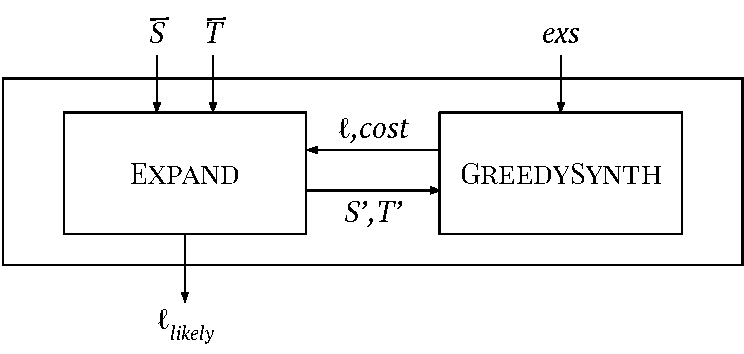
\includegraphics[width=.5\textwidth]{high-level-algorithm.pdf}
%  \caption{Schematic Diagram for \SOptician. Regular expressions \Regex and
%    \RegexAlt, and a set of examples \Examples, are provided as input. \RXSearch
%    searches through stochastic regular expression pairs, equivalent to the
%    originals, and proposes them to \GreedySynth. \GreedySynth finds a lens,
%    typed between the generated equivalent pairs. When \RXSearch determines it
%    has an optimal lens, it returns that lens.}
%  \label{fig:high-level-algorithm}
%\end{figure}
%
%\bcp{It gets rather technical and incomprehensible for the next three
%  paragraphs...} 
%
%We develop an algorithm that synthesizes a low-cost lens, shown in
%Figure~\ref{fig:high-level-algorithm}. This algorithm consists of two
%communicating synthesizers, one that proposes candidate stochastic regular
%expression pairs that it thinks will align well, and one that greedily searches
%for a lens between those two regular expressions that minimizes cost and does
%not traverse star-related equivalences\bcp{???}. When the first algorithm is content with
%the lens it has found, it returns that lens. 
%
%\bcp{Make clear that these algorithms are based on earlier / published ones.}Our first algorithm, \RXSearch, proposes candidate stochastic regular
%expressions. These candidate stochastic regular expressions are generated by
%traversing \emph{star semiring} equivalences on stochastic regular expressions.
%These proposed stochastic regular expression pairs have equivalent languages and
%probability distributions as the original ones: we prove that the star-semiring
%rewrites this synthesizer applies are sound rewrites on stochastic regular
%expressions.
%
%Our second algorithm, \GreedySynth, utilizes alternative languages for
%stochastic regular expressions and lenses, \emph{stochastic DNF regular
%  expressions} and \emph{symmetric DNF lenses}. While these languages are hard
%to read and understand, they are highly normalized and permit an efficient
%type-directed synthesis algorithm. We develop our cost metric on DNF lenses, and
%provide a greedy algorithm that tries to find a symmetric DNF lens of minimal
%cost. The synthesized symmetric DNF lens is then converted to a lens in the
%original simple symmetric lens language.
%
%
%We evaluate our algorithm on a benchmark suite consisting of synchronizing file
%formats from configuration files, application-specific data storage files, and
%data cleaning tasks. We find that our algorithm is able to synthesize each of
%these lenses in under 20 seconds.
%
%In summary, our contributions are:
%\begin{enumerate}
%\item We develop \emph{simple symmetric lenses} a new formulation for
%  bidirectional programs that can project data from both sides~(\S\ref{sec:overview}),
%  and describe a language that expresses such lenses on string
%  data~(\S\ref{sec:ssl}).  \bcp{A new language, or a variant of
%    Hofmann/Pierce/Wagner?} 
%\item We develop a means to traverse stochastic regular expression equivalences,
%  while preserving probability distributions and
%  languages~(\S\ref{subsec:stoch-rx}).
%\item We develop stochastic DNF regular expressions and DNF
%  lenses~(\S\ref{subsec:greedy-synth}). We develop a sound algorithm for
%  converting stochastic regular expressions to stochastic DNF regular
%  expressions and a information-theoretic cost metric on DNF lenses.
%\item We extended Boomerang with our simple symmetric lens combinators, and
%  integrated our algorithm with the Optician synthesis system within Boomerang,
%  allowing synthesis tasks as Boomerang
%  expressions~(\S\ref{sec:implementation}).
%\item We evaluate our algorithm on a benchmark suite consisting of synchronizing
%  file formats from configuration files, application-specific data storage
%  files, and data cleaning tasks (\S\ref{sec:evaluation}).  \bcp{... and
%    conclude what?}
%\end{enumerate}

%%% Local Variables:
%%% TeX-master: "main"
%%% End:
